\section{Detector Installation}
\label{sec:fdsp-tc-inst}

%This section describes the baseline installation plan to assemble the \dword{apa}, \dword{ce}, and \dword{pd} in a surface facility. The installation team is investigating in parallel the possibility of performing the work underground. A decision will be made as to what is the optimal course of action prior to the TDR being finalized.

%The \dword{dune} detector installation will proceed in three phases: the \dword{cuc} set up, the installation set up, and the detector installation. Figure \ref{fig:high-level-schedule} shows the major underground activities and gives an idea of what work will be occurring in which phase. \dword{cuc} set up is the first step in the installation process. The phase begins when the underground area for the north cavern and central cavern become available to \dword{lbnf} and \dword{dune}. At this time, the cryostat construction can begin in the north cavern, and \dword{dune} equipment installation can begin in the central cavern or \dword{cuc}. Figure~\ref{fig:cavern-layout} shows a top view of the underground areas. The equipment from \dword{dune} installed in this phase is the infrastructure in the \dword{dune} dataroom. Figure~\ref{fig:cavern-layout} shows he dataroom in the \dword{cuc} on the west end of the excavation. The detector installation setup phase (referred to as Infrastructure Det\#1 in Figure \ref{fig:cavern-layout}) begins during the cryostat membrane installation period. In this phase, the equipment needed for detector installation will be erected in north cavern. This includes installing the bridge across the cavern, the cleanroom, lifting equipment and work platforms, the coldboxes, and the cryogenic system for testing \dword{apa}, and the \dword{dss} with the related switchyard. In the third phase of the installation, the detector itself will be installed. The work in each phase will be described the following sections.

As mentioned in Section~\ref{sec:fdsp-tc-log}, the \dword{dune} detector installation will proceed in three phases: the \dword{cuc} set up, the installation set up, and the detector installation. Figure \ref{fig:high-level-schedule} shows the major underground activities and gives an idea of what work occurs in each phase. 

\dword{cuc} set up is the first step in the installation process. The phase begins when the underground area for the north cavern and central cavern become available to \dword{lbnf} and \dword{dune}. At this time, the \dword{lbnf} cryostat construction can begin in the north cavern, and \dword{dune} equipment installation can begin in the \dword{cuc}. Figure~\ref{fig:cavern-layout} shows a top view of the underground areas. The \dword{dune} equipment  installed in this phase is the infrastructure in the \dword{dune} dataroom. Figure~\ref{fig:cavern-layout} shows the dataroom in the \dword{cuc} on the west end of the excavation. 

The detector installation setup phase (referred to as Infrastructure Det\#1 in Figure \ref{fig:high-level-schedule}) begins during the cryostat membrane installation period. In this phase, the equipment needed for detector installation is erected in the north cavern. This includes the bridge across the cavern, the cleanroom, lifting equipment and work platforms, the \coldbox{}es, and the cryogenics system for \dword{apa} testing, and the \dword{dss} and switchyard. 

The detector itself is installed in the third phase of the installation. 

\begin{dunefigure}[Layout of the DUNE underground areas]{fig:cavern-layout}
  {Top view of the layout at the 4850 level at SURF. Shown are the three large excavations and the location of detectors in excavations \#1 and \#3. Excavation \#2 is the CUC, which houses the DUNE dataroom and the underground utilities.}
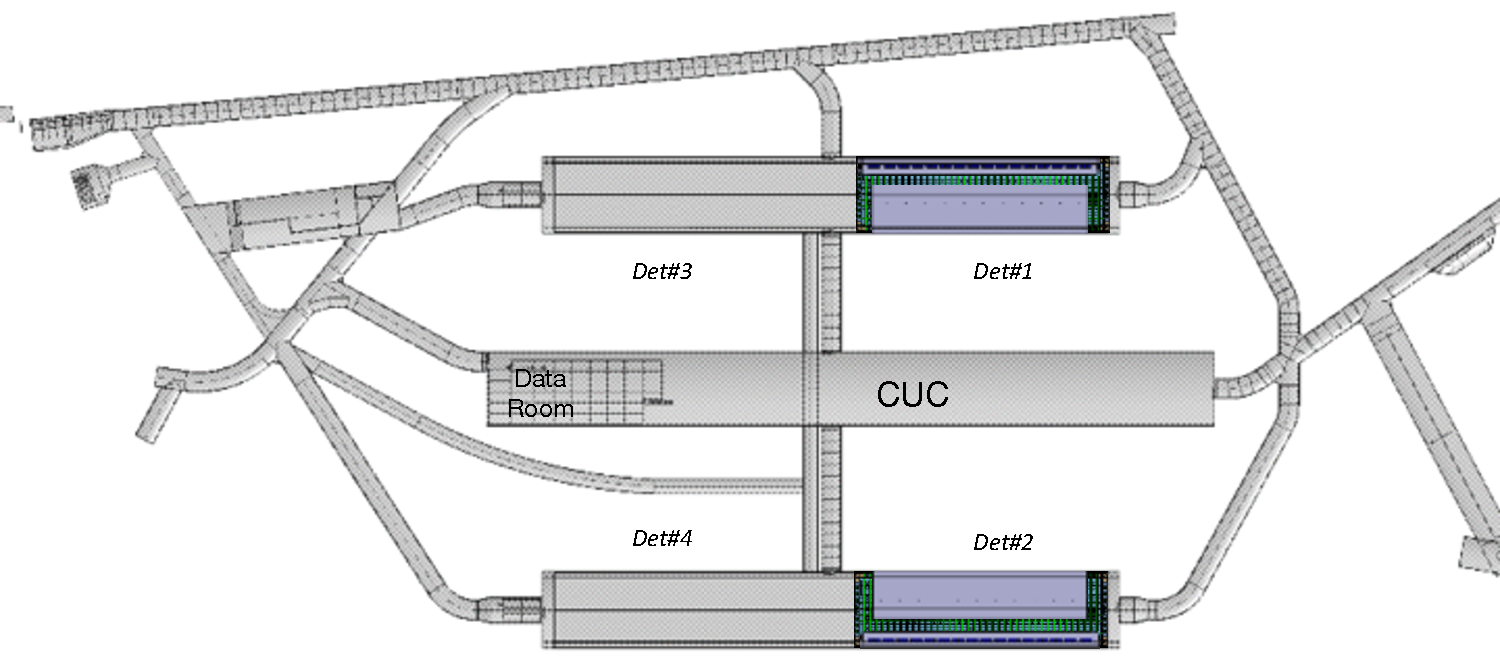
\includegraphics[width=.9\textwidth]{cavern-layout}
\end{dunefigure}

\begin{dunefigure}[High level installation  schedule]{fig:high-level-schedule}
  {Overview schedule showing the main activities underground.}
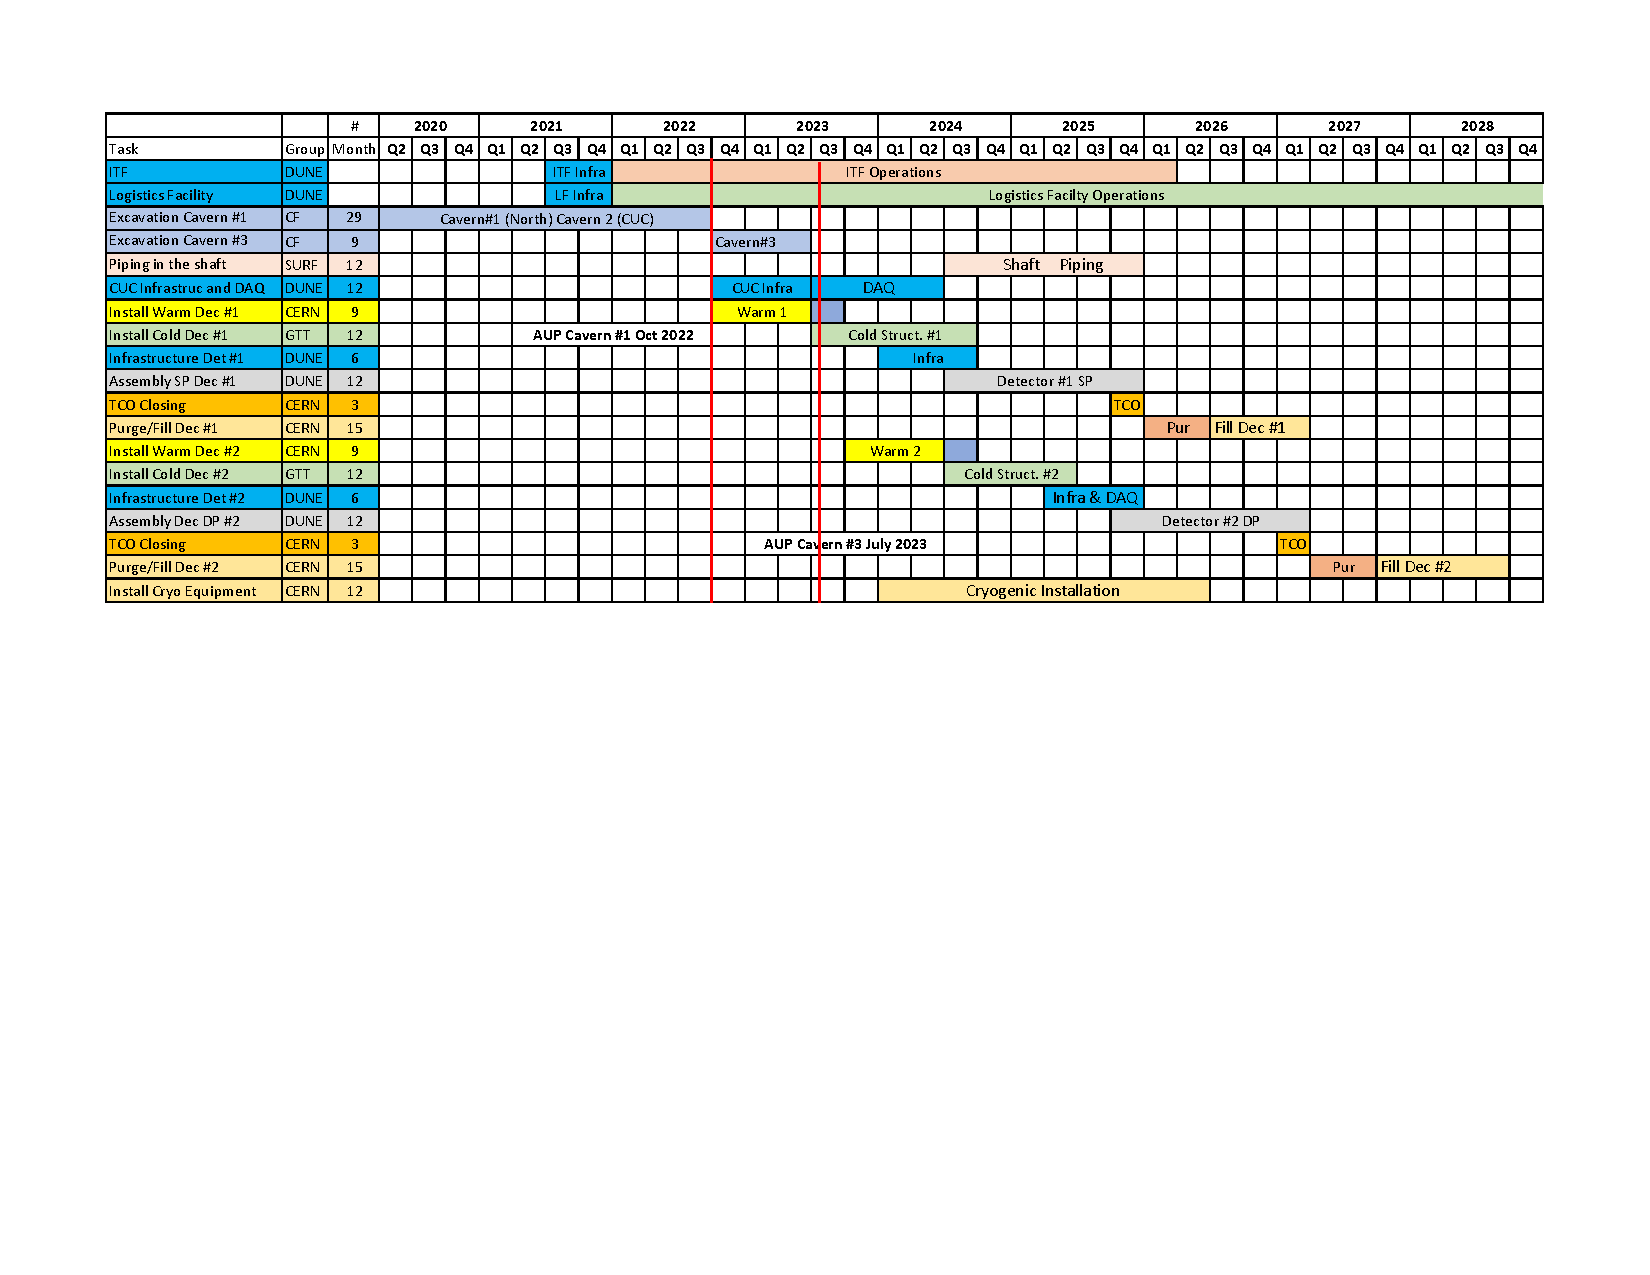
\includegraphics[width=.99\textwidth]{high-level-schedule}
\end{dunefigure}

%%%%%%%%%%%%%%%%%%%%%%%%%%%%
\subsection{Installation Process Description}
\label{sec:fdsp-tc-inst-proc}


%The work performed in each of the three installation phases (\dword{cuc} installation phase, installation setup phase and the detector installation phase) are described in each of the following three subsections.

\subsubsection{CUC Installation Phase}
\label{sec:fdsp-tc-inst-CUC}

\begin{dunefigure}[Layout of the DUNE data room and work area in CUC]{fig:install-cuc}
  {Top: The overall layout of the \dword{dune} spaces in the \dword{cuc}. A110 is the DUNE data room, which houses the underground computing, and A111 is a general purpose work area (not a control room as labeled) that we call the experimental work area. Bottom: The first row of ten racks in the data room is shown. The first two represent the \dword{cf} interface racks. The images were taken from the ARUP 90\% design drawings U1-FD-A-108 and U1-FD-T-701.}
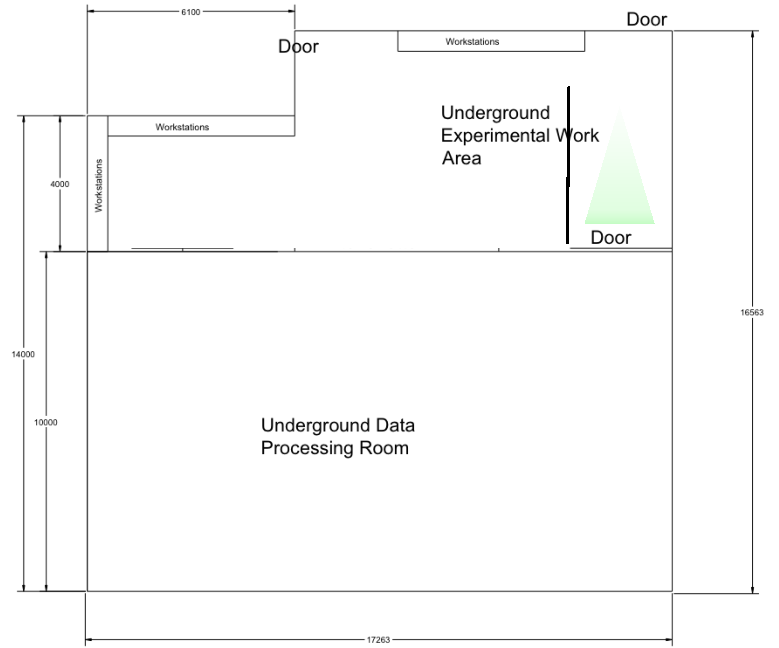
\includegraphics[width=.85\textwidth]{cuc-layout}
\vspace{-2pt}
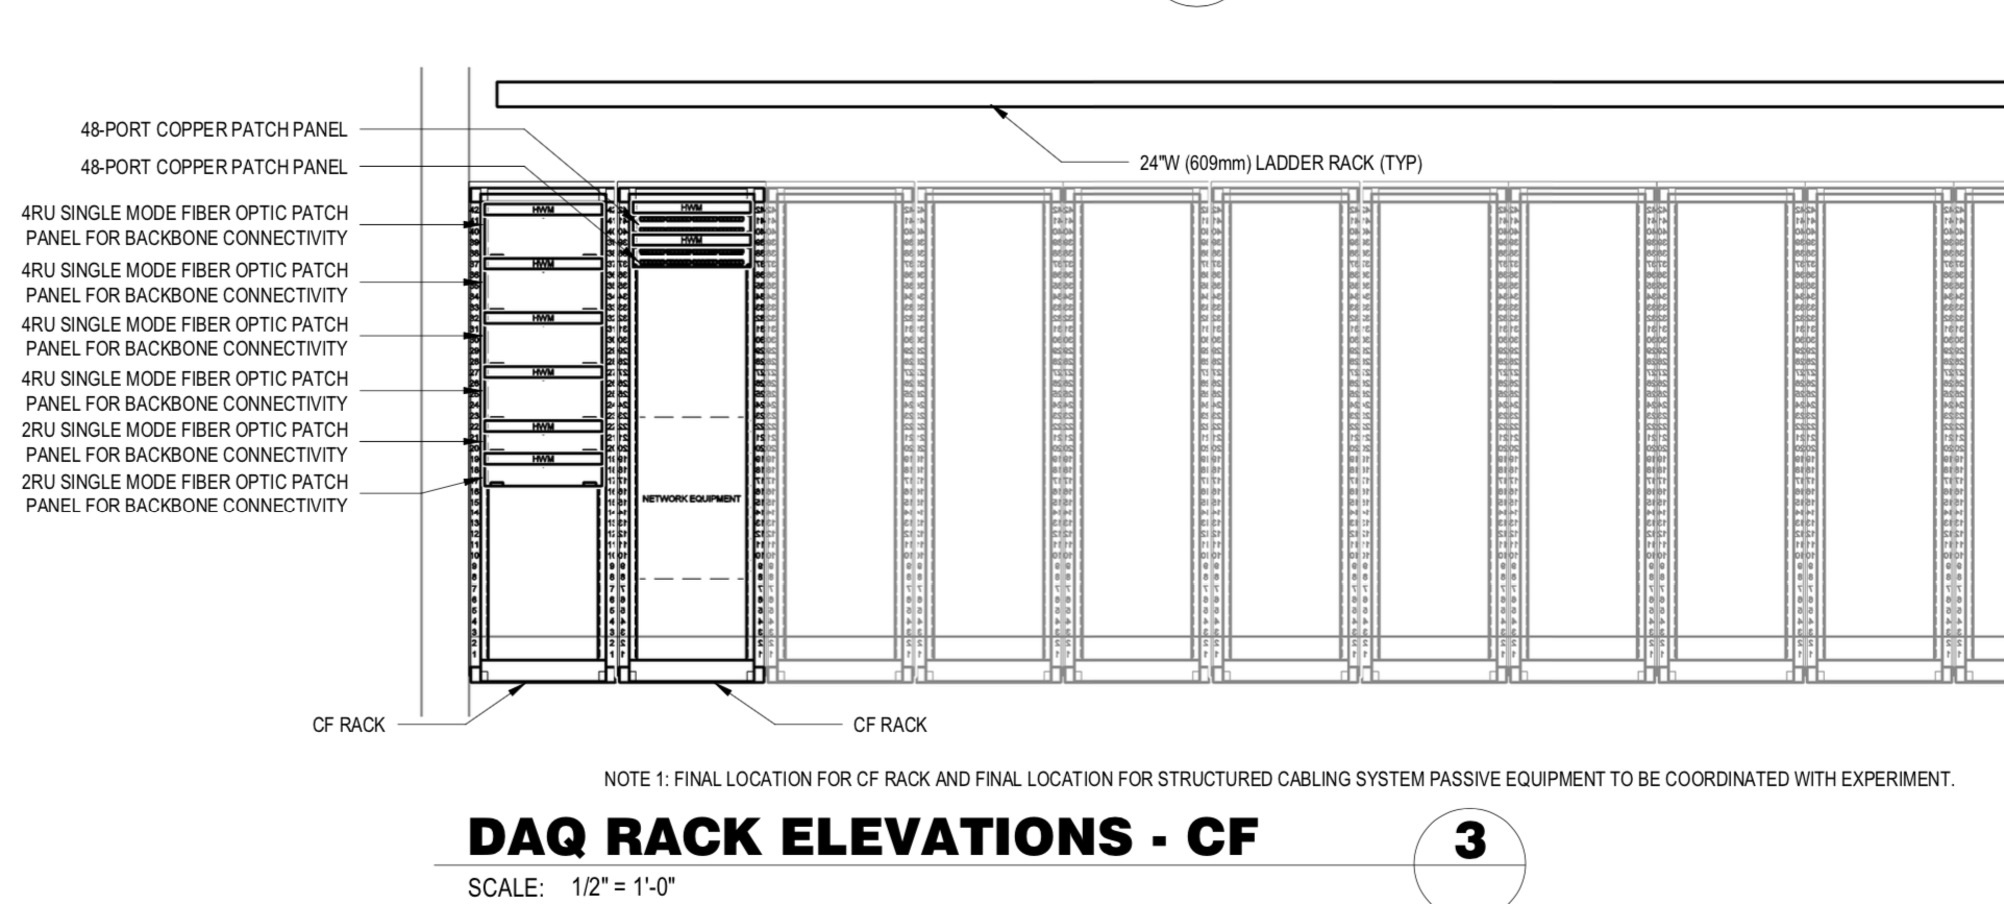
\includegraphics[width=.9\textwidth]{cuc-cf-racks}
\end{dunefigure}

%The first stage of the \dword{cf} work ends when outfitting the north and central caverns is complete. At this time, the \dword{cuc} is ready for \dword{dune} outfitting, and the cryostat installation can start for detector \#1. At this time \dword{dune} will not have assess to the detector excavations because the heavy steel work for the cryostat will be ongoing. The only work planned for \dword{dune} in this period is the outfitting of the dataroom and work area room in the \dword{cuc} shown in Figure~\ref{fig:install-cuc}.  \dword{cf} is providing redundant single mode fiber up the shafts to provide external connectivity.  \dword{cf} is also providing the empty dataroom with an 18 \si{in} false floor, a 500 \si{kVA} power disconnect, and connections for sufficient chilled water to cool the racks. The dataroom, like the adjacent \dword{cf} electronics room, will be outfitted with a dry fire extinguishing system. 
Once the \dword{lbnf} \dword{cf} outfitting of the north cavern and the \dword{cuc} is complete,  \dword{lbnf} begins the first cryostat installation in the north cavern and \dword{dune} can begin to install equipment in the dataroom and work area room in the \dword{cuc}. See Figure~\ref{fig:install-cuc}.  \dword{dune} will not have access to the north cavern due to the heavy steel work for the cryostat. 
At this point \dword{lbnf}  \dword{cf} will have installed redundant single-mode fiber up the shafts to provide external connectivity, and in the empty dataroom,  an \SI{18}{in} false floor, a \SI{500}{kVA} power disconnect, and connections for sufficient chilled water to cool the racks. The dataroom, like the adjacent \dword{cf} electronics room, will be outfitted with a dry fire extinguishing system. 
 

The water-cooled racks, cable trays, power distribution, and water distribution are the responsibility of \dword{dune} and will be installed once the space becomes available. The \dword{daq} fiber trunk between the detector cavern and the \dword{cuc} dataroom will be installed %later when 
after the cable trays are available in the north cavern. Installation of the racks must be coordinated with \dword{cf} %because 
since the first two racks are for \dword{cf} use and must be in place before the first phase of %one 
work underground is complete. Some small overlap will be needed between \dword{cf} and \dword{dune} at this time. The general purpose network will be installed by \dword{fnal}'s \dword{sdsd} and connected to the shaft fiber. This is required for most %further 
subsequent work in the underground area.


%Data from the detector electronics will be transmitted over a multimode fiber trunk from the warm interface boards on top the detector to the \dword{daq} dataroom in the \dword{cuc} shown in Fig.~\ref{fig:install-cuc}.  This room will contain 60 water cooled racks, two of which are reserved for \dword{cf} use, two for \dword{cisc} servers, and the rest for \dword{daq} servers and networking. Although this is the total number of racks needed for all four detector modules, the racks themselves will be installed at the beginning of the \dword{cuc} commissioning phase because they must be plumbed into the cooling water below the dataroom's drop floor and wired into power distribution from the ceiling.  \dword{daq} equipment will populate the racks as needed for servicing the detector commissioning.  For the first detector module, details of this configuration will be informed by knowledge gained from \dword{daq} vertical slice tests done at other institutions.  
Data from the detector electronics will be transmitted over a multimode fiber trunk from the \dwords{wib} on top the \dword{spmod} to the \dword{daq} data room in the \dword{cuc}, shown in Figure~\ref{fig:install-cuc}.  The data room will contain 60 water-cooled racks, two of which are reserved for \dword{cf} use, two for \dword{cisc} servers, and the rest for \dword{daq} servers and networking. Racks for all four modules will be installed at the beginning of the \dword{cuc} commissioning phase because they must be plumbed into the cooling water below the dataroom's drop floor and wired into power distribution from the ceiling.  \dword{daq} equipment will populate the racks as needed for servicing the detector commissioning.  For the first detector module, details of this configuration will be informed by \dword{daq} vertical slice tests done at other institutions.  

At the same time, the eight above-ground \dword{daq} racks that receive data from the underground data room and  transmit the data to \dword{fnal} will %also 
be installed, connected to the WAN, and connected to the single-mode fiber in the Ross and Yates Shafts.  With this infrastructure in place, the \dword{daq} group can begin constructing and testing the final \dword{dune} \dword{daq}, starting with the %.  The 
timing system. % is the first \dword{daq} component needed.  
Enough \dword{daq} back-end servers to support the first \dword{apa}s will be operational before the \dword{apa}s are installed.  The remainder of the \dword{daq} will grow in parallel with \dword{apa} installation.

%The underground experimental work area (referred to in Figure \ref{fig:install-cuc} as CONTROL ROOM) is a general purpose area that must serve many purposes during the \dword{dune} installation. Initially, the area will be outfitted with office equipment for the installation team, workstations for \dword{daq}, and a basic conference area for meetings. The room is 5.5 - 8 \si{m} deep and 17 \si{m} wide, so it can serve several functions.
The underground experimental work area (shown as ``CONTROL ROOM'' in Figure~\ref{fig:install-cuc}) must serve a variety of purposes during the \dword{dune} installation. Initially, the area will be outfitted with office equipment for the installation team, workstations for \dword{daq}, and a basic conference area for meetings. The room is 17 \si{m} wide with portions that are \SI{5.5}{m} and \SI{8}{m} deep.

During this early installation stage, the machine shop and \dword{dune} storage area will %also 
be set up in the detector excavation area and %. These facilities will be 
shared with the cryostat team. 

\subsubsection{Installation Setup Phase}
\label{sec:fdsp-tc-inst-setup}

Once the steel structure of the cryostat is complete, the remaining work by the \dword{lbnf} cryostat team will be focused inside the cryostat installing the insulation and membrane.  
\dword{lbnf} activity outside the cryostat will %relate 
consist mainly of %to 
transporting the 4,000 crates of foam and other materials from the cavern to inside the cryostat. %Since the cryostat outer steel structure will, however, be in position, so some \dword{dune} work can start. 
Since the cryostat outer steel structure will be in position, \dword{dune} can install 
%The 
the first piece of equipment, % to be installed will be t
he bridge between the north and south drifts. 
This will allow the cryogenics equipment to travel from the north drift to the \dword{cuc} and will provide part of the structure for the cleanroom. 
Construction of the cleanroom frame and related hoisting equipment can then begin. 


\fixme{Start: from Cleanroom Infrastructure in infrastructure.tex}
The assembly of the detector sub-components into \SI{12}{m} tall full assemblies %modules 
must be done underground directly outside the cryostat. The full %12 \si{m} long 
assemblies are too large and fragile to be brought down the shaft, and the only place with enough vertical space to assemble them is in front of the cryostat itself. A combination of contractors and the lead worker and rigger teams will do the infrastructure work; they will also assist in detector assembly. The cleanliness requirement for all work on the components inside the detector means that all work must be done in an ISO-8 cleanroom, so a very large cleanroom must be built outside the cryostat containing all the necessary infrastructure to assemble the %detector \dword{tpc} elements. 
\dword{lartpc} components. Figure \ref{fig:cleanroom-layout} illustrates %provides an image of 
the conceptual design of the installation cleanroom. The left figure is an end view of the cleanroom, showing the materials airlock 
\fixme{at the back (east end) ?} 
and the changing room. The right image is a side view showing the cleanroom on the left and the airlock on the right.

The plan is to bring all detector elements into the cleanroom through large roll up doors in the side wall of the airlock. The materials will be moved using using  a battery operated forklift and electric pallet jacks. The airlock will be  13 \si{m} wide 10 \si{m} deep and 17 \si{m} tall. This is large enough to hold the \dword{apa} assembly tower described below with enough extra space to move large objects inside. An access hatch is planned for the roof, allowing the cavern bridge crane to be used in the central area of the airlock. The crane is needed to manipulate the \dword{apa} modules in the airlock. %; the plan calls for assembly of the double-high \dword{apa} pairs there. 
Also shown on the right of the figure is the changing room for the cleanroom. The changing room is 3 \si{m} wide and 10 \si{m} deep. The dimensions were chosen to allow 20-30 people to gown up for the cleanroom within a reasonable time. The requirements for work in an ISO-8 cleanroom are a cleanroom lab coat, clean shoes, and nets for hair and beards.  This will be augmented with a clean hard hat and gloves for safety reasons. 

The outline of the cleanroom proper is shown on the right in Figure \ref{fig:cleanroom-layout}. The cleanroom dimensions are 16 \si{m} wide 10 \si{m} deep and 17 \si{m} tall. The cleanroom lies primarily under the north-south bridge and in the 3.4 m space between the bridge and the cryostat. %Here operations that must be performed are the 

\fixme{start: line 162 from infrastructure file}
Cabling of the \dword{apa}, cold testing of the \dword{apa}, and assembly of the cathode \dword{fc} modules will take place here. The tower for the \dword{apa} cabling, the \coldbox{}es for testing, and the switchyard for moving the 12m tall objects are described below. All areas of the airlock and cleanroom will be outfitted with UV filtered lights. In addition to this cleanroom, the inside of the cryostat will also be effectively a cleanroom.  By filtering the air and forcing it  into the cryostat at the east end, the clean air will flow through the cryostat and out through the cleanroom and airlock. This will keep the inside of the cryostat at least at ISO-8. The construction process for the cleanroom is still at the conceptual level so what is shown is a steel frame structure where panels can be mounted. %The size is substantial and the occupancy significant, so the cleanroom should have electrical outlets, UV filtered lighting, and fire protection. 
Given the substantial size and the significant occupancy, the cleanroom will have electrical outlets, UV filtered lighting, and fire protection. 

\fixme{need to check all dimensions and update the figure}

\begin{dunefigure}[APA assembly tower]{fig:apa-assemble-frame}
  {The \dword{apa} assembly tower with the \dword{apa} assembly frame attached. The transport rails at the top of the figure are used to move the assembled \dword{apa} into the cleanroom. The work decks allow access to the \dword{apa} from multiple levels. }
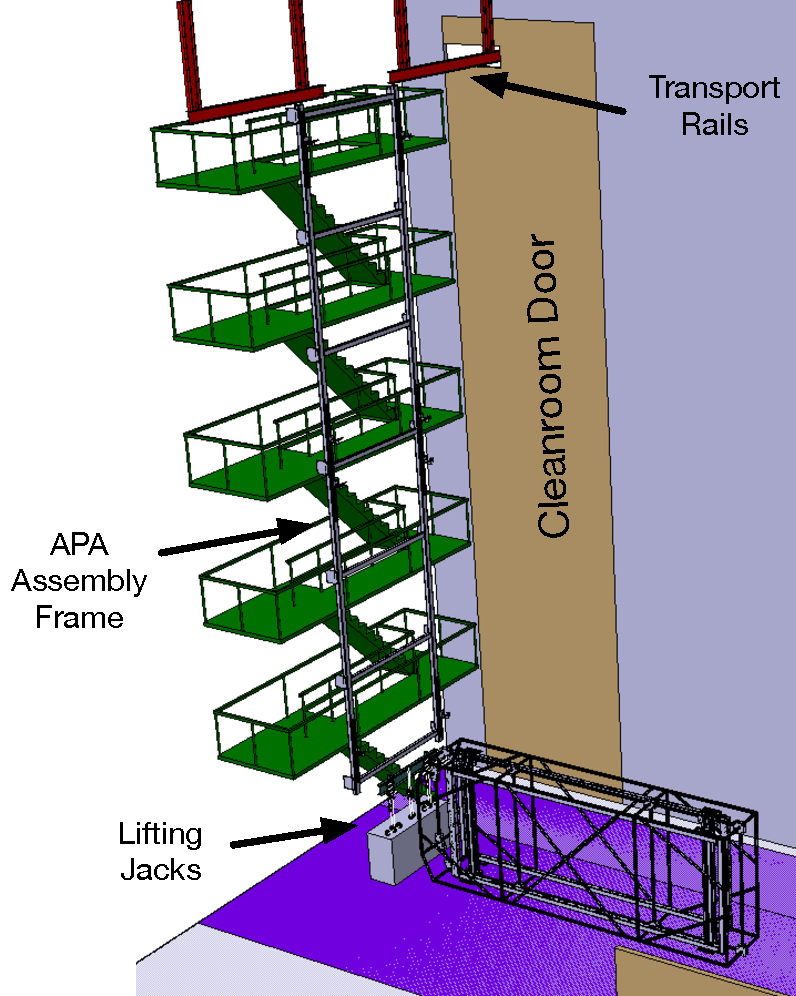
\includegraphics[width=.5\textwidth]{apa-assemble-frame}
\end{dunefigure}
\fixme{end from infrastructure file}
\fixme{Maybe here is where you want the APA-CE-PD Integration section from itf.tex \ref{sec:fdsp-tc-itf-integ}.  Actually  you may want to split this chapter -- there's a lot of integration info to incorporate from itf.tex. }


Cabling of the \dword{apa}, cold testing of the \dword{apa}, and assembly of the cathode \dword{fc} modules will take place here. The tower for the \dword{apa} cabling, the \coldbox{}es for testing, and the switchyard for moving the 12m tall objects are described below. All areas of the airlock and cleanroom will be outfitted with UV filtered lights. In addition to this cleanroom, the inside of the cryostat will also be effectively a cleanroom.  By filtering the air and forcing it  into the cryostat at the east end, the clean air will flow through the cryostat and out through the cleanroom and airlock. This will keep the inside of the cryostat at least at ISO-8. The construction process for the cleanroom is still at the conceptual level so what is shown is a steel frame structure where panels can be mounted. %The size is substantial and the occupancy significant, so the cleanroom should have electrical outlets, UV filtered lighting, and fire protection. 
Given the substantial size and the significant occupancy, the cleanroom will have electrical outlets, UV filtered lighting, and fire protection. 
\fixme{End: from Cleanroom Infrastructure in infrastructure.tex}




The largest, most complex equipment to be constructed in this phase are the \coldbox{}es and %related 
the associated cryogenics system. 
%Because the coldboxes are so large, they must be constructed in place. 
The \coldbox{}es, visible in Figure \ref{fig:install-cleanroom-layout}, must be constructed in place due to their size.  
%Figure \ref{fig:install-cleanroom-layout} shows the layout of the installation region outside the cryostat. 
This figure also %shows a cut \fixme{shows a cut?} 
is a view from below the bridge (not shown) so that most of the installation equipment can be seen. 
The three \SI{15}{m} tall  \coldbox{}es are shown in blue next to the yellow access stairway. 

The hoisting equipment and the rail system for moving the detector components into the installation area interfaces with the bridge, cryostat, and possibly the cleanroom mechanical structure. 
Installing this early will make transporting equipment around the area outside the cryostat significantly easier. 
 
%The assembly towers for the \dword{apa} assembly, \dword{apa} cabling, and \dword{cpa} assembly can be installed when it is most convenient for the cryostat installation crew. Just before starting to install the detector, the cleanroom walls will be installed, the area will be cleaned, and added filters will be installed to convert the area to an ISO-8 cleanroom.
The assembly towers for the \dword{apa} assembly, \dword{apa} cabling, and \dword{cpa} assembly can be installed at the convenience of the cryostat installation crew. Once they are in place, the cleanroom walls are installed, the area is cleaned, and added air filters are installed to convert the area to an ISO-8 cleanroom. This must be completed before detector installation can begin.

During this time %period 
most of the cryostat installation work takes place inside the cryostat at the bottom (4910 level) and  %This implies that 
the cryostat roof is available to the \dword{lbnf} and \dword{dune} installation teams to complete  
%This will allow 
much of the work for installing the cyrogenics system and setting up for the detector installation.  %set up to be performed in parallel to the cryostat work. 


\begin{dunefigure}[Installation of electronics crosses]{fig:install-elect-cross}
  {Installation of the crosses to which the \dword{ce} warm readout and the \dword{pd} cables are connected.}
 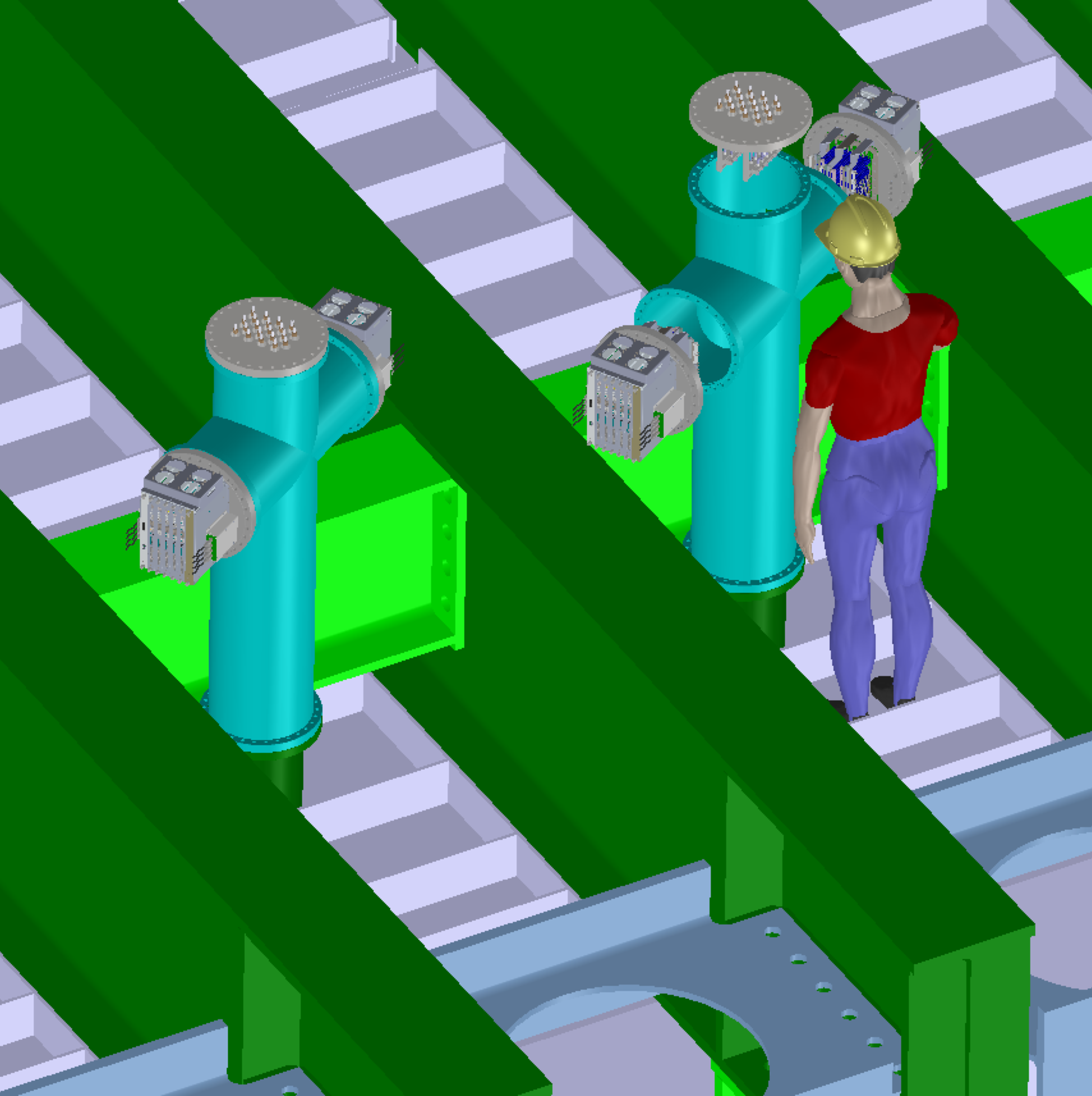
\includegraphics[width=.75\textwidth]{install-elect-cross}
\end{dunefigure}

%The cryostat crossing tubes will be installed on the roof as required by the cryostat assembly sequence. 
The first step is installation of the cryostat crossing tubes, which will follow the cryostat assembly sequence.  \fixme{x-ref to where this is outlined. } 
These assemblies are welded to the \SI{1}{cm} thick steel cryostat roof and %are then additionally 
cross braced to the large I-Beams. 
The thin-walled tubes that penetrate %through 
the foam insulation are welded in place at this time. 

Once the crossing tubes are installed and leak chased, \fixme{leak checked?} % the \dword{ce} crosses can be connected and the feedthrough flanges for the \dword{ce} and \dword{pd} can be mounted onto the crosses. Figure \ref{fig:install-elect-cross} shows the set up. 
we connect the  \dword{ce} crosses and mount  the feedthrough flanges for the \dword{ce} and \dwords{pd} onto the crosses. 
The height of the crosses was chosen to allow a person to work comfortably on the \dwords{wec}  and \dword{pd} flanges while standing on the cryostat roof. 
A fully assembled cross is shown on the left of Figure~\ref{fig:install-elect-cross}, and a cross with a \dword{wec} outside the assembly position is shown on the right. 
The present plan is to install the crosses shortly after the cryostat crossing tubes are installed. 
%By doing this, the 
This allows us to seal the large openings in the cryostat roof % can be sealed, and 
and easily achieve cleanroom conditions %can easily be achieved 
after the cryostat is cleaned. 
For this stage, temporary seals %will be 
are used for the flanges because they must be removed during the cabling process later in the installation. At this time, the 
dword{ce} mechanical feedthroughs can also be installed. 

\begin{dunefigure}[DSS feedthrough installation]{fig:install-dss-feedthru}
  {The \dword{dss} support feedthroughs are installed using a gantry crane running along the roof of the cryostat. The cryostat decking is not shown %in this figure 
  but the gantry %will be able to 
  can move freely on the cryostat roof decking. The gantry crane is selected to fit under the mezzanine as shown in the right panel.}
  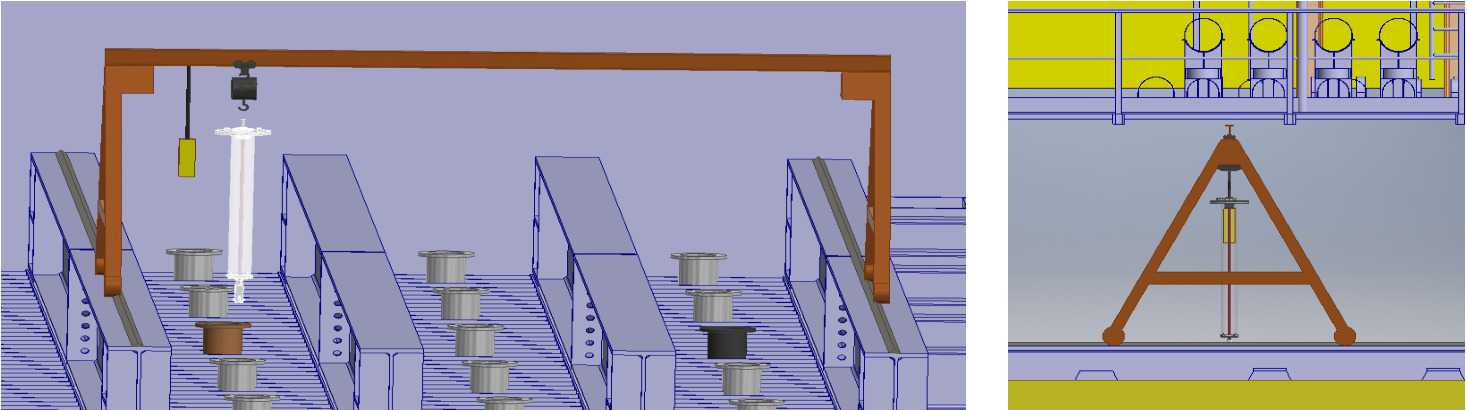
\includegraphics[width=.98\textwidth]{graphics/install-dss-feedthru-v2.pdf}
 %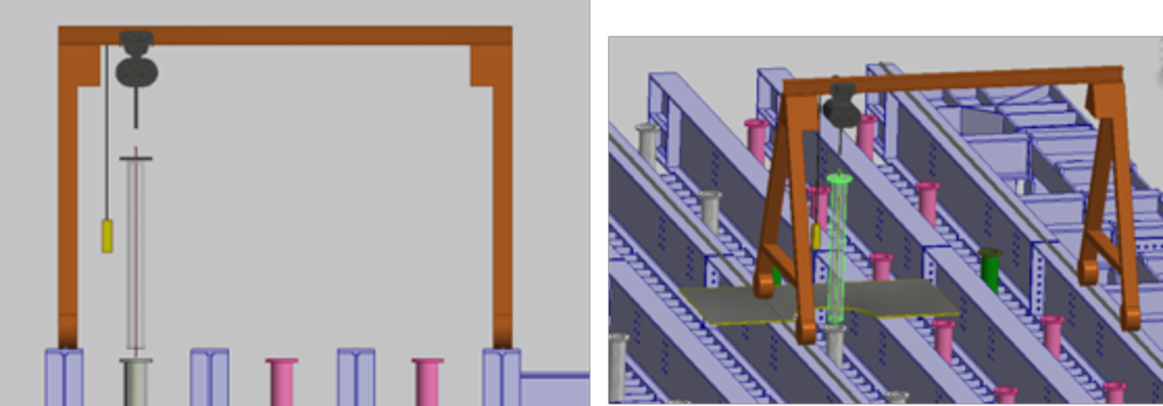
\includegraphics[width=.95\textwidth]{graphics/dss-feedthru-install.pdf}
\end{dunefigure}

%When the crossing tube installation is complete, and in parallel to the installation of the \dword{ce} tees, the \dword{dss} support feedthroughs can be installed. A gantry crane on top of the cryostat picks up the feedthroughs and feeds them into the cryostat crossing tubes as shown in Figure \ref{fig:install-dss-feedthru}. This is the first step in the \dword{dss} installation.There are \num{20} \fdth{}s per row and five rows for a total of \num{100} \fdth{}s.  A fixture with a tooling ball is attached to theclevis of each \fdth.  The $xy$ position in the horizontal planeand the vertical $z$ position of this tooling ball is defined, then a  survey is performed to determine the location of each tooling ball center, and $xy$ and $z$ adjustments are made to get the toolingball centers to within $\pm$\SI{3}{mm}.  The \SI{6.4}{m} long I-beams are then raised and pinned to the clevis.  Each beam weighs roughly \SI{160}{kg} (\SI{350}{lbs}).A lifting tripod is placed over each of the \fdth{}s supporting a beam, and a \SI{0.64}{cm} (\SI{0.25}{in})  %$1/4 ^{''}$  cable is fed through the top flange of the \fdth down \SI{14}{m} to the cryostat floor where it is attached to the I-beam. The cable access port and lifting cable are shown in Figure \ref{fig:dss-beam-lifting}. 
%The winches on each tripod raise the beam in unison to position it at the correct height to be pinned to the \fdth clevis.  Once the beams are mounted, a final survey of the beams ensures they are properly located and aligned to each other.
The \dword{dss} support feedthroughs can be installed in parallel to the \dword{ce} crosses. This is the first step in the \dword{dss} installation. A gantry crane on top of the cryostat picks up the feedthroughs and feeds them into the cryostat crossing tubes as shown in Figure \ref{fig:install-dss-feedthru}. There are \num{20} \fdth{}s per row and five rows, for a total of \num{100} \fdth{}s.  A fixture with a tooling ball is attached to the clevis of each \fdth{}.  The horizontal $xy$ and the vertical $z$ positions of this tooling ball are defined, survey is performed to determine the location of each tooling ball center, and adjustments are made to get the tooling ball centers to within $\pm$\SI{3}{mm}. \fixme{of what?}  The \SI{6.4}{m} long I-beams are then raised and pinned to the clevis.  Each beam weighs roughly \SI{160}{kg} (\SI{350}{lbs}). A lifting tripod is placed over each  \fdth{}'s supporting beam, and a \SI{0.64}{cm} (\SI{0.25}{in})  %$1/4 ^{''}$  
cable is fed through the top flange of the \fdth down \SI{14}{m} to the cryostat floor where it is attached to the I-beam. The cable access port and lifting cable are shown in Figure \ref{fig:dss-beam-lifting}. 
The winches on each tripod raise the beam in unison to position it at the correct height for pinning to the \fdth clevis.  Once the beams are mounted, a final survey of the beams ensures proper placement and alignment. 
 \begin{dunefigure}[DSS I-Beam lifting setup]{fig:dss-beam-lifting}
  {A cable access port is included in the \dword{dss} flange. This is used to feed a cable from the roof through the flange and attach it to the I-beams during \dword{dss} installation.}
 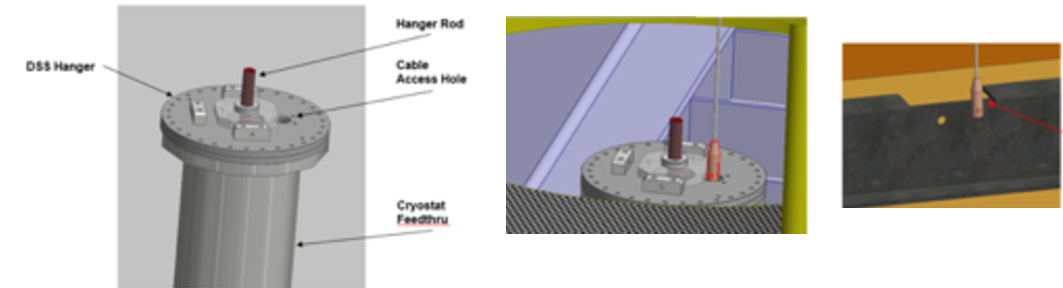
\includegraphics[width=.95\textwidth]{graphics/dss-beam-lifting.pdf}
\end{dunefigure}

%Once work on the feedthroughs is complete, then the mezzanines for the cryogenics system and the detector electronics racks can be installed. Finally, the cable trays,  piping, lighting, and cryostat roof flooring are installed. At this time, the cryostat roof is ready for \dword{daq} installation to begin in the detector area, which will proceed in parallel to the detector installation.
Next it is time to install the mezzanines for the cryogenics system and the detector electronics racks, followed by installation of the cable trays,  piping, lighting, and cryostat roof flooring. At this point, the cryostat roof is ready for \dword{daq} installation to begin; this will proceed in parallel to the detector installation.

The last steps in the installation setup phase involve installing the cryostat internal piping, cleaning the cryostat, installing the false floor, and installing filtered lighting to protect the \dwords{pd}.  \fixme{include air filtering here?} The false floor gives both a flat work area and protects the \SI{1.2}{mm} thick stainless steel cryostat membrane. 


\subsubsection{Detector Installation Phase}
\label{sec:fdsp-tc-inst-execute}

\begin{dunefigure}[Top view of the installation region inside the cleanroom ]{fig:install-cleanroom-layout}
  {Top view of the cleanroom used for installation. In this view, cleanroom roof and bridge are not shown. The equipment used for installation is shown along with the material airlock layout and the location of the changing room. The cryostat is to the right of the figure and the I-beams passing through the TCO opening are shown.}
 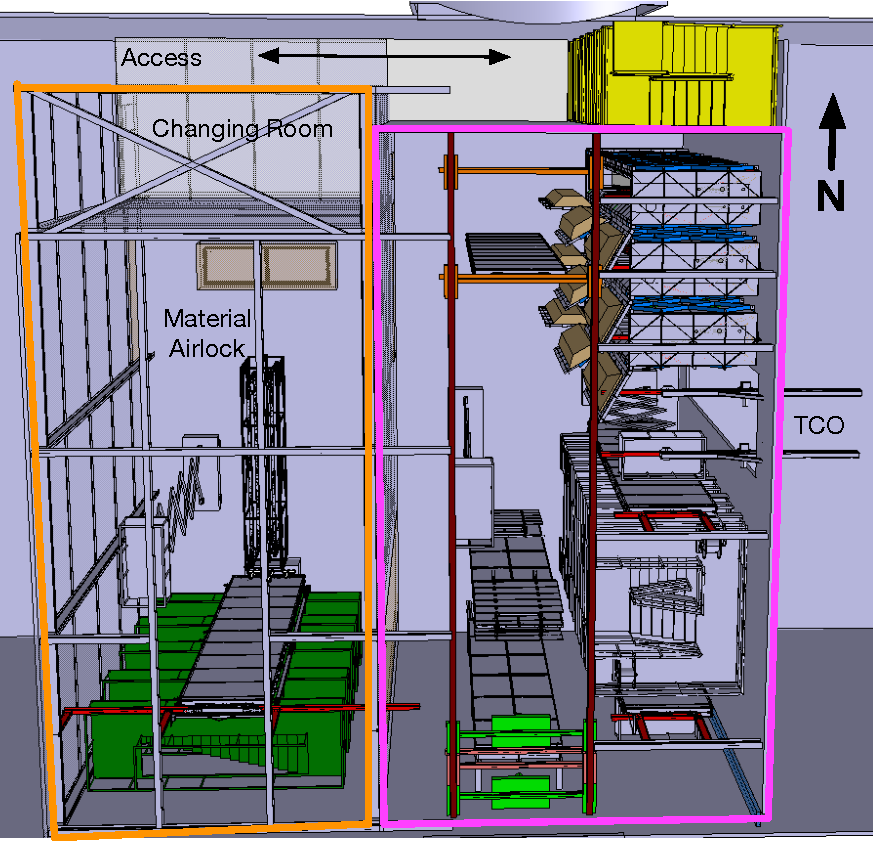
\includegraphics[width=\textwidth]{install-cleanroom-layout}
\end{dunefigure}

%At the start of the detector installation phase, when the work on the cleanroom is complete, the \dword{dss} is installed in the cryostat including the switchyard near the \dword{tco}. The lighting in the cryostat and cleanroom will be filtered to protect the \dwords{pd}, and the air will be filtered to reduce the dust collected during installation. The cryogenic piping and the false floor will be in place. The false floor gives both a flat work area and protects the 1.2 \si{mm} thick stainless steel cryostat membrane. 
\fixme{a bunch of this pgraph repeated the end of prev section}
The detector installation phase begins when the work on the cleanroom is complete, starting with installation of the  \dword{dss} in the cryostat along with the switchyard near the \dword{tco}. 
          
%Figure \ref{fig:install-cleanroom-layout} shows the layout of the cleanroom during the detector installation phase. This image is a top view of the cleanroom with the roof and bridge removed; the cryostat is on the right and the open cavern on the left. In the north-east corner of the figure, the access stairway is shown in yellow. This stairway is outside the cleanroom and allows people to access the 4910 level from the north drift or from the cryostat roof. An access corridor along the north wall connects the stairway to the rest of the cavern. The changing room and materials airlock are on the west of the figure and are outlined in orange. The changing room is in the the northwest corner and provides access to both the cleanroom and the airlock. South of the changing room is the material airlock. This rather large area is where the \dword{apa} modules are connected to form the 12 \si{m} tall units. The assembly station is shown in green along the south wall of the airlock. This area is also where all materials are brought from the dirty outside cavern and where they are cleaned or the outer packaging removed. Roll-up doors along the west wall allow material from the outer cavern to be brought into the airlock. A section of the roof can be removed to allow the cavern bridge crane to manipulate the \dword{apa} transport boxes and modules. The cleanroom area itself is shown on the right of the figure and is outlined in magenta. Inside the cleanroom is a switchyard material transport system (shown in red) similar to what is used for the \dword{dss} inside the cryostat. The switchyard is used to move the assembled detector components north-south in the cleanroom. East-west rail sections are then used to deliver the components to the required work location. In the north area of the cleanroom are the three coldboxes used to cryogenically test the fully assembled and cabled \dword{apa} pairs. In the south half of the cleanroom is the \dword{apa} cabling tower used for cabling and testing the \dword{apa} pairs. Along the south wall is the \dword{cpa} assembly fixture for assembling the \dword{cpa}. 

Figure \ref{fig:install-cleanroom-layout} shows the layout (plan view) of the cleanroom during the detector installation phase with the roof and bridge removed; the cryostat is on the right and the open cavern on the left. In the north-east corner of the figure, the access stairway is shown in yellow. This stairway is outside the cleanroom and allows people to access the 4910 level (bottom of cryostat) from the north drift or from the cryostat roof. An access corridor along the north wall connects the stairway to the rest of the cavern.  The changing room is in the the northwest corner and provides access to both the cleanroom and the airlock.
%
 South of the changing room is the material airlock where the \dword{apa} pairs are connected \fixme{this must be where PDs and CE are installed now???}  to form the \SI{12}{m} tall units. The  \dword{apa} assembly station is shown in green along the south wall of the airlock. This area is also where all materials are brought from the outside cavern and cleaned or unpacked. The materials pass  into the airlock through roll-up doors along the west wall. A section of the roof can be removed to allow the cavern bridge crane to manipulate the \dword{apa} transport boxes and modules. \fixme{what modules?} 
 %
The cleanroom area is shown on the right, outlined in magenta. Inside the cleanroom is a switchyard material transport system (shown in red) similar to what is used for the \dword{dss} inside the cryostat. The switchyard is used to move the assembled detector components north-south in the cleanroom. East-west rail sections deliver the components to the required work locations. The north area of the cleanroom houses the three \coldbox{}es. The \dword{apa} cabling tower is in the south half of the cleanroom.  The \dword{cpa} assembly fixture is along the south wall.  
 
%Labor for the detector installation phase has two main components: The \dword{uit} that includes a scientific lead, manager, two deputy managers (one on each shift), safety officer, and administrative help. They are responsible for communicating with the \dword{itf} and logistics facility to ensure needed components are shipped underground and kept properly in the inventory system.  They also organize/plan daily tasks done underground with the lead workers and rigging teams as well as the different consortia.  Several teams of three \dword{fte} consisting of a lead worker and riggers responsible for moving all \dword{tpc} components into the materials airlock,  cleanroom, coldbox, and cryostat. An additional team (lead--worker, riggers and technicians) works in the cryostat to position the \dword{tpc} components and deploy the \dwords{fc} during the final stage of each new drift volume. 
Labor for the detector installation phase is split between two groups: The \dword{uit} that includes a scientific lead, manager, two deputy managers (one on each shift), a safety officer, and administrative help. They are responsible for communicating with the logistics facility to ensure needed components are shipped underground and properly maintained in the inventory system.  They also organize and plan daily underground tasks with the lead workers and rigging teams, as well as the different consortia.  Several teams of three \dword{fte}, consisting of a lead worker and riggers, are responsible for moving all \dword{tpc} components into the materials airlock,  cleanroom, \coldbox, and cryostat. An additional team (lead worker, riggers and technicians) works in the cryostat to position the \dword{tpc} components and, during the final stage of each new drift volume,  deploy the \dwords{fc}. 

%The second labor component includes the different consortia with specific tasks related to each individual group. These labor estimates will be refined during the \dword{dune}-Ash River trial assembly work as we do time and motion studies. Figure \ref{fig:Single-APA-Schedule} below shows a typical labor breakdown in the \dword{sas}, cleanroom, and cryostat. The \dword{apa} installation was chosen for this example.
The second group comprises the \dword{fd} consortia, each with specific tasks related to its subsystem. Figure \ref{fig:Single-APA-Schedule} shows a typical labor breakdown in the airlock,  cleanroom, and cryostat. These labor estimates will be refined during time and motion studies at Ash River. The \dword{apa} installation was chosen for this example.  

\begin{dunefigure}[Typical APA installation schedule]
{fig:Single-APA-Schedule}
{Typical \dword{apa} schedule for \dword{spmod}}
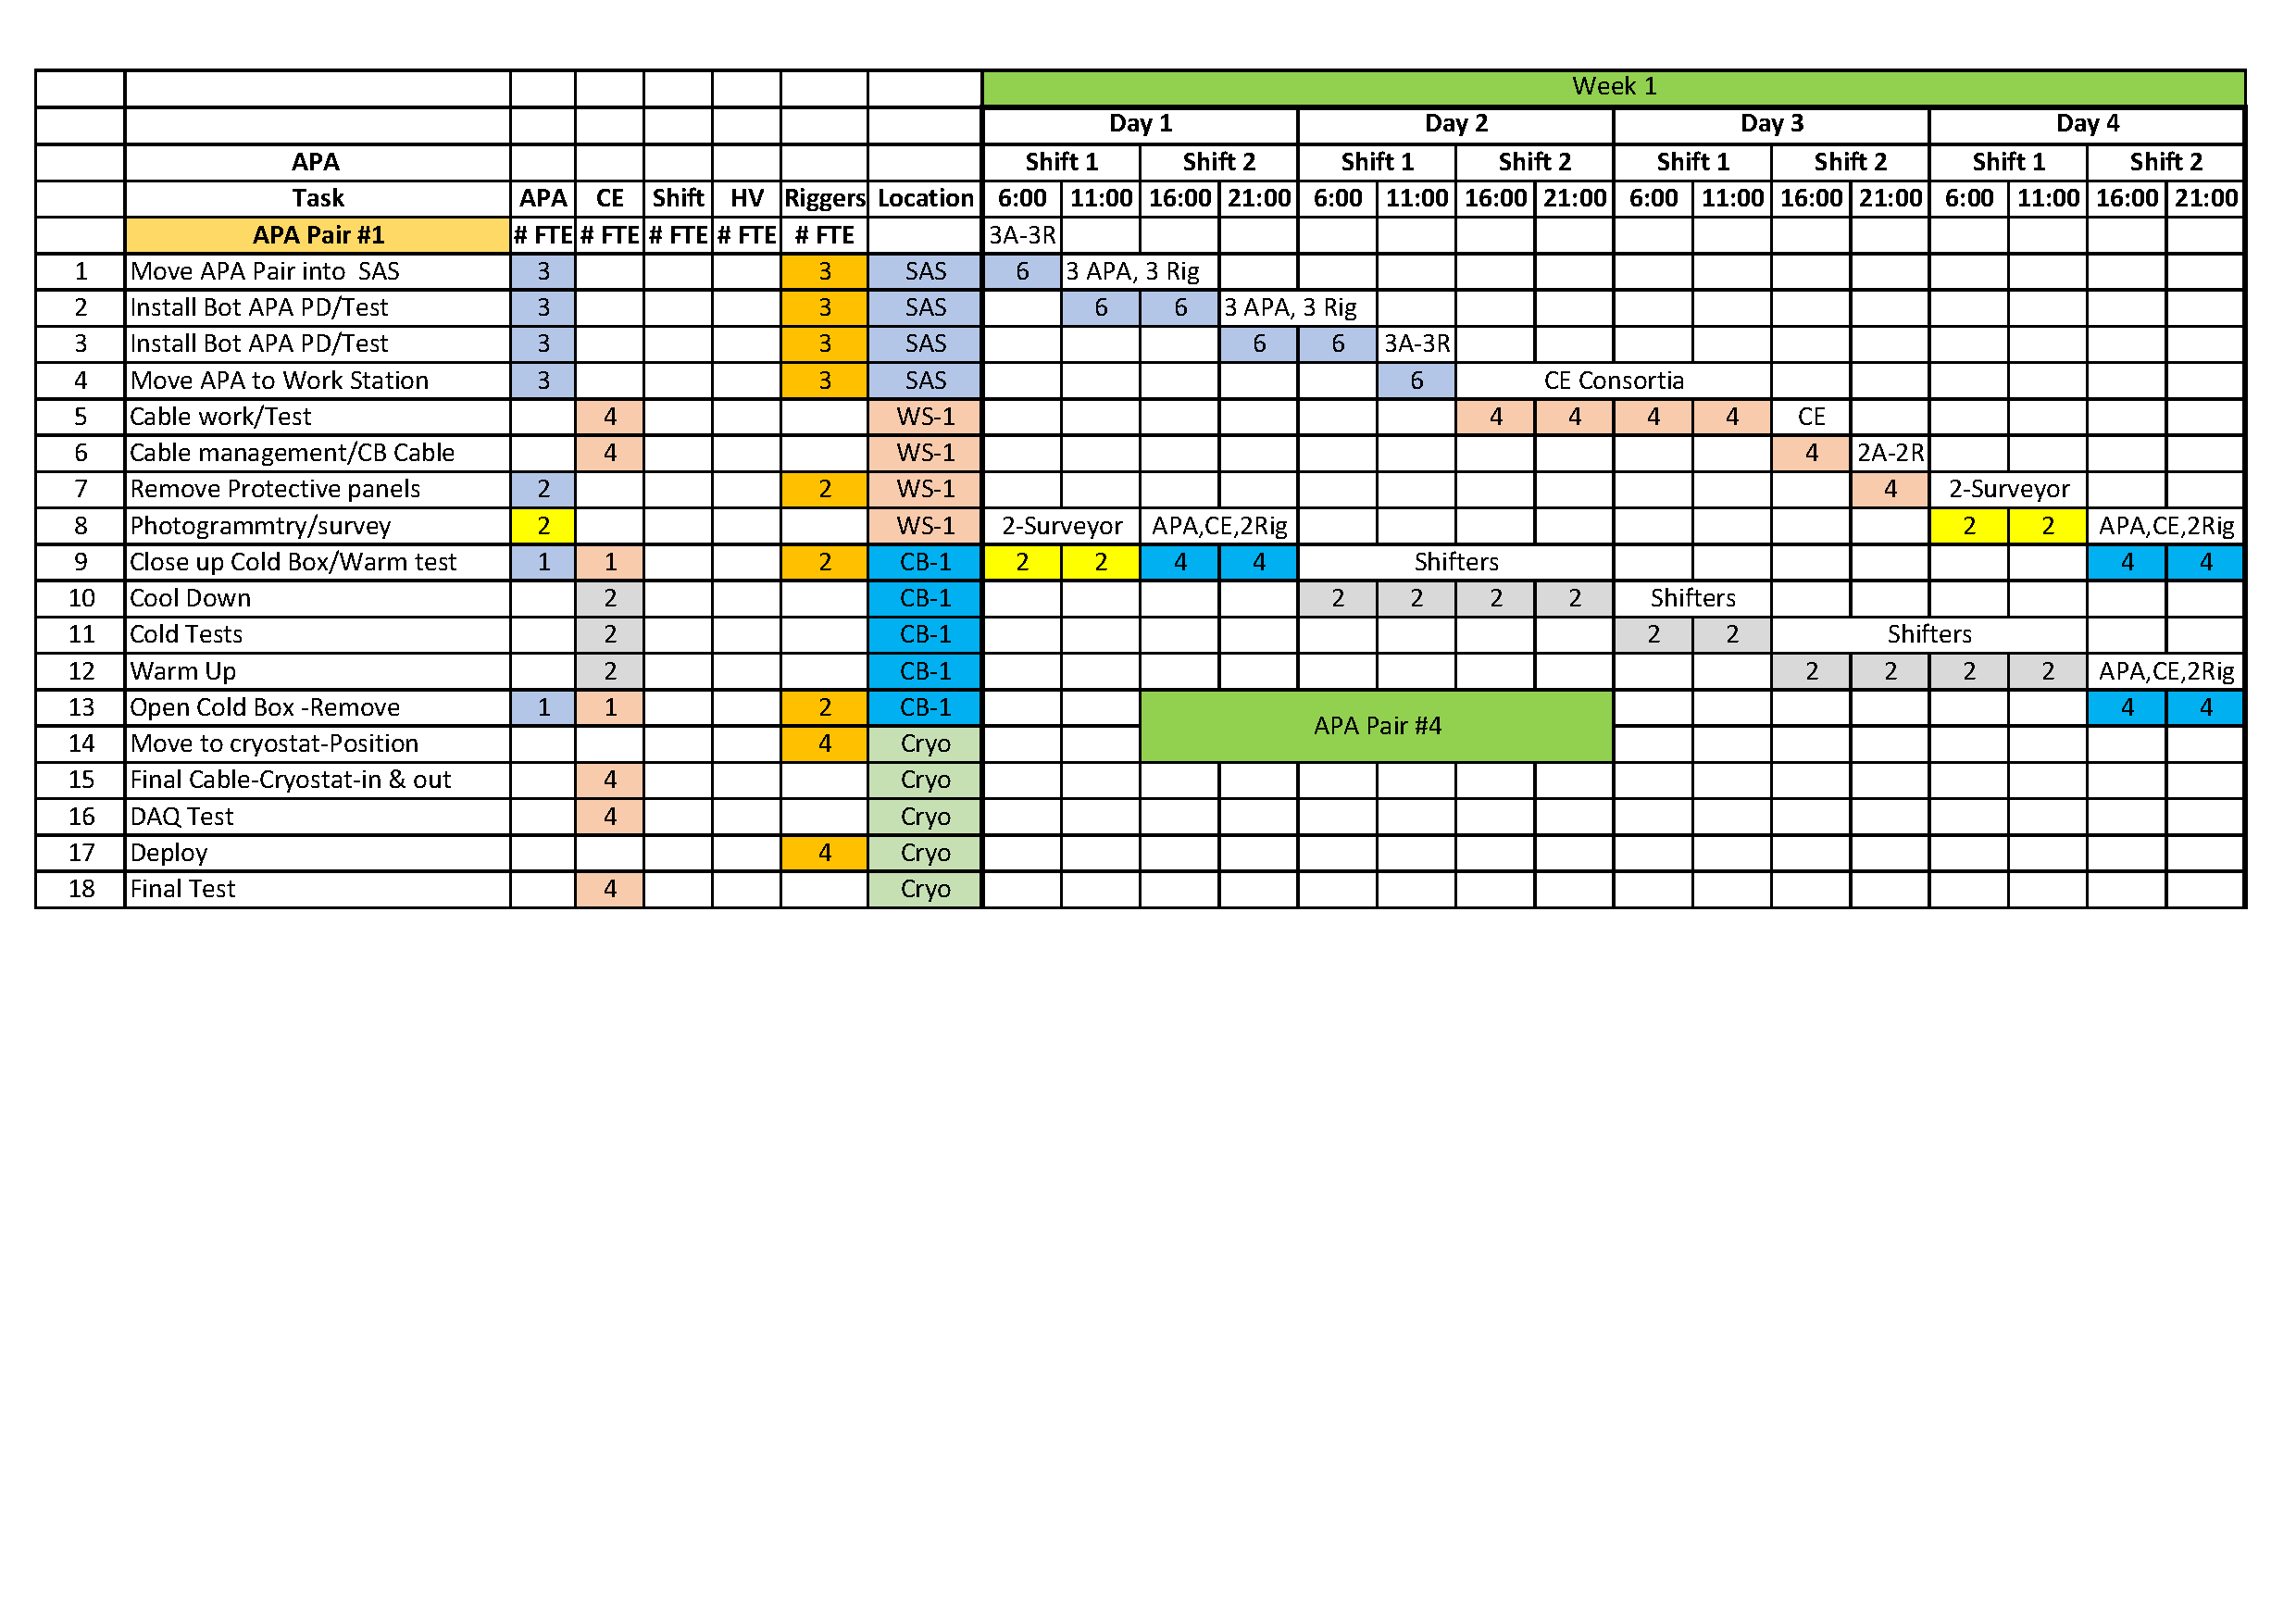
\includegraphics[width=0.95\textwidth]{Single-APA-Schedule.pdf}
\end{dunefigure}
\fixme{text in figure is very small - rotate 90 deg?}

\begin{dunefigure}[Design of the instrumentation feedthroughs]{fig:CISC-feedthru}
{The signal feedthrough is integrated with the DSS support feedthroughs. A side port on a short spool piece in the DSS support structure allows the instrumentation cables to be fed through the cryostat walls where needed.}
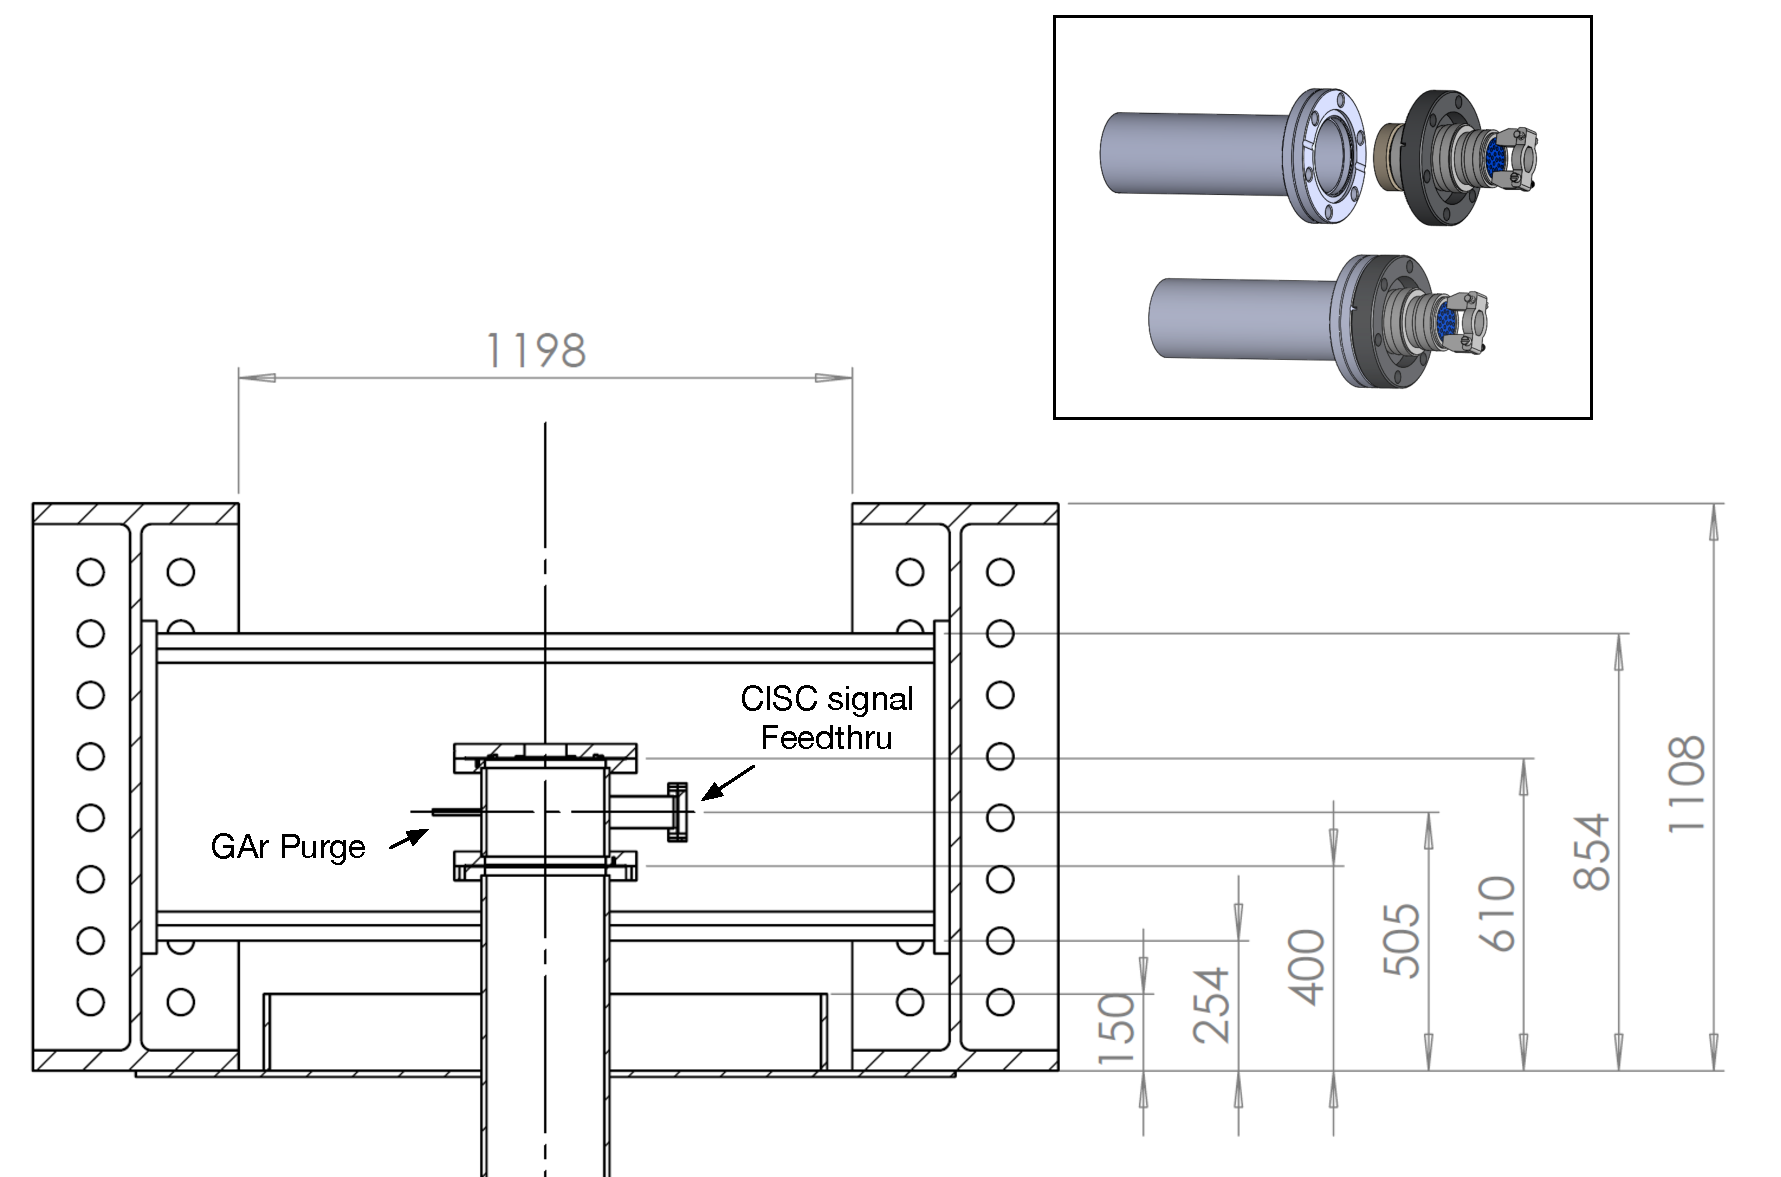
\includegraphics[width=0.95\textwidth]{CISC-feedthru.pdf}
\end{dunefigure}



%The first detector equipment to be installed are CISC thermometers,\fixme{SG: I think "CISC thermometers" is confusing since CISC has several types of thermometers. I assume here you mean static T-gradient thermometers? If so, clarify that.} one array of purity monitors, and cameras at the east end of the cryostat. This equipment will be used to monitor the cool down, filling, and commissioning of the detector. Some equipment for the laser calibration system will also be installed at this time including some positioning diodes and possibly a optical mirror based switching system. Because these components are small, they can be installed using a scissor lift with 12 \si{m} reach. At present, this is the tallest battery operated (thus cleanroom compatible) scissor lift rated for use in the USA that we have identified. The signals exit the cryostat using electrical feedthroughs distributed across the cryostat roof and integrated with the \dword{dss} support structure as shown in Figure \ref{fig:CISC-feedthru}.
The first detector equipment to be installed are \dword{cisc} T-gradient thermometers, \fixme{SG: T-gradient correct? anne} an array of purity monitors, and cameras at the east end of the cryostat. This equipment will be used to monitor the cool down, filling, and commissioning of the detector. Some equipment for the laser calibration system is also installed at this time,  including some positioning diodes and possibly an optical mirror-based switching system.  The signals exit the cryostat using electrical feedthroughs distributed across the cryostat roof and integrated with the \dword{dss} support structure, as shown in Figure \ref{fig:CISC-feedthru}. Because all these components are small, they can be installed using a scissor lift with 12 \si{m} reach. At present, this is the tallest battery operated (thus cleanroom compatible) scissor lift rated for use in the USA that we have identified.

%Cabling for the static T-gradient monitors must be installed before the outer \dword{apa}s, so we plan to install them also during the early installation period. The thermometer system will be supported using the bolts at the top and bottom of the cryostat. To avoid any damage, the sensors will be plugged into the IDC-4 connectors later, just before moving the corresponding \dword{apa} into its final position. Individual sensors on pipes and the cryostat floor are installed immediately after installing the static T-gradient monitors. Cables with their corresponding supports are installed first, and sensors are installed later, just before unfolding the bottom \dwords{gp}, to avoid any damage. Individual sensors on the top \dword{gp} must be integrated with the other \dwords{gp}. For each \dword{cpa} (with its corresponding four \dword{gp} modules) going inside the cryostat, cable and sensor supports will be anchored to the \dword{gp} threaded rods. Once the \dword{cpa} is moved into its final position and its top \dwords{gp} are ready to be unfolded, sensors on these \dwords{gp} are installed.
\fixme{Following pgraph needs work}
Cabling for the static T-gradient monitors is also installed early, before the outer \dword{apa}s.  The thermometer system is supported using the bolts at the top and bottom of the cryostat. To avoid  damage, the \fixme{which?} sensors are not plugged into the IDC-4 connectors until just before the corresponding \dword{apa} is moved into its final position. Individual sensors on pipes and the cryostat floor are installed immediately after installing the static T-gradient monitors. \fixme{this makes no sense to me - sounds like you can step on them!} Cables \fixme{for apa, pd, cpa?} with their corresponding supports are installed first,\fixme{first after what?} and \fixme{which?} sensors are installed later, just before unfolding the bottom \dwords{gp}, to avoid damage. Individual sensors on the top \dword{gp} must be integrated with the other \dwords{gp}. For each \dword{cpa} (with its corresponding four \dword{gp} modules), cable and sensor supports will be anchored to the \dword{gp} threaded rods. Once the \dword{cpa} is moved into its final position and its top \dwords{gp} are ready to be unfolded, sensors on these \dwords{gp} are installed.

%Installing fixed cameras is, in principle, simple but involves a large number of interfaces. The enclosure for each camera has exterior threaded holes to facilitate mounting the camera on the cryostat wall, cryogenic internal piping, or \dword{dss}. Each enclosure is attached to a gas line to maintain appropriate underpressure in the fill gas, so an interface with cryogenic internal piping will be necessary. Camera cables will be run through cable trays to flanges on assigned instrumentation feedthroughs. 
Installing fixed cameras is, in principle, simple but involves a large number of interfaces. The enclosure for each camera has exterior threaded holes to facilitate mounting the camera on the cryostat wall, cryogenic internal piping, or \dword{dss}. Each enclosure is attached to a gas line to maintain appropriate underpressure in the fill gas, requiring an interface with cryogenic internal piping. Camera cables are run through cable trays to flanges on assigned instrumentation feedthroughs. 


A summary of all the cryogenics instrumentation provided by the \dword{cisc} consortium is shown in Figure~\ref{fig:cisc_devices}. 

%The quartz optical fibers required for the \dword{pd} monitoring system will be pre-installed at this point as well.  Fibers will be run from the optical flange locations (which are still being finalized) to locations on the \dword{cpa} support structures, to be connected to the diffusers mounted on the \dword{cpa}s during installation.
At this point the quartz optical fibers required for the \dword{pd} monitoring system are   run from the optical flange locations (still being finalized) to locations on the \dword{cpa} support structures, to be connected later to the diffusers mounted on the \dword{cpa}s.

%The residual gas analyzers that monitor for impurities in the gaseous argon system must be installed before the piston purge and gas recirculation phases of cryostat commissioning. The exact timing of the gas analyzers will depend on the schedule for outfitting the mezzanine and installing the gaseous argon purge piping. The instruments are installed near the tubing switchyard to minimize tubing run length and for convenience when switching the sampling points and gas analyzers. 
The residual gas analyzers that monitor for impurities in the \dword{gar} system must be installed before the piston purge and gas recirculation phases of cryostat commissioning. \fixme{doesn't everything?} The  timing will depend on the schedule for outfitting the mezzanine and installing the  \dword{gar} purge piping. The instruments are installed near the tubing switchyard to minimize tubing run length and for convenience when switching the sampling points and gas analyzers. 

\begin{dunefigure}[Distribution of various \dword{cisc} devices inside the cryostat.]{fig:cisc_devices}
  {Distribution of various %instrumentation 
  \dword{cisc} devices inside the cryostat}
  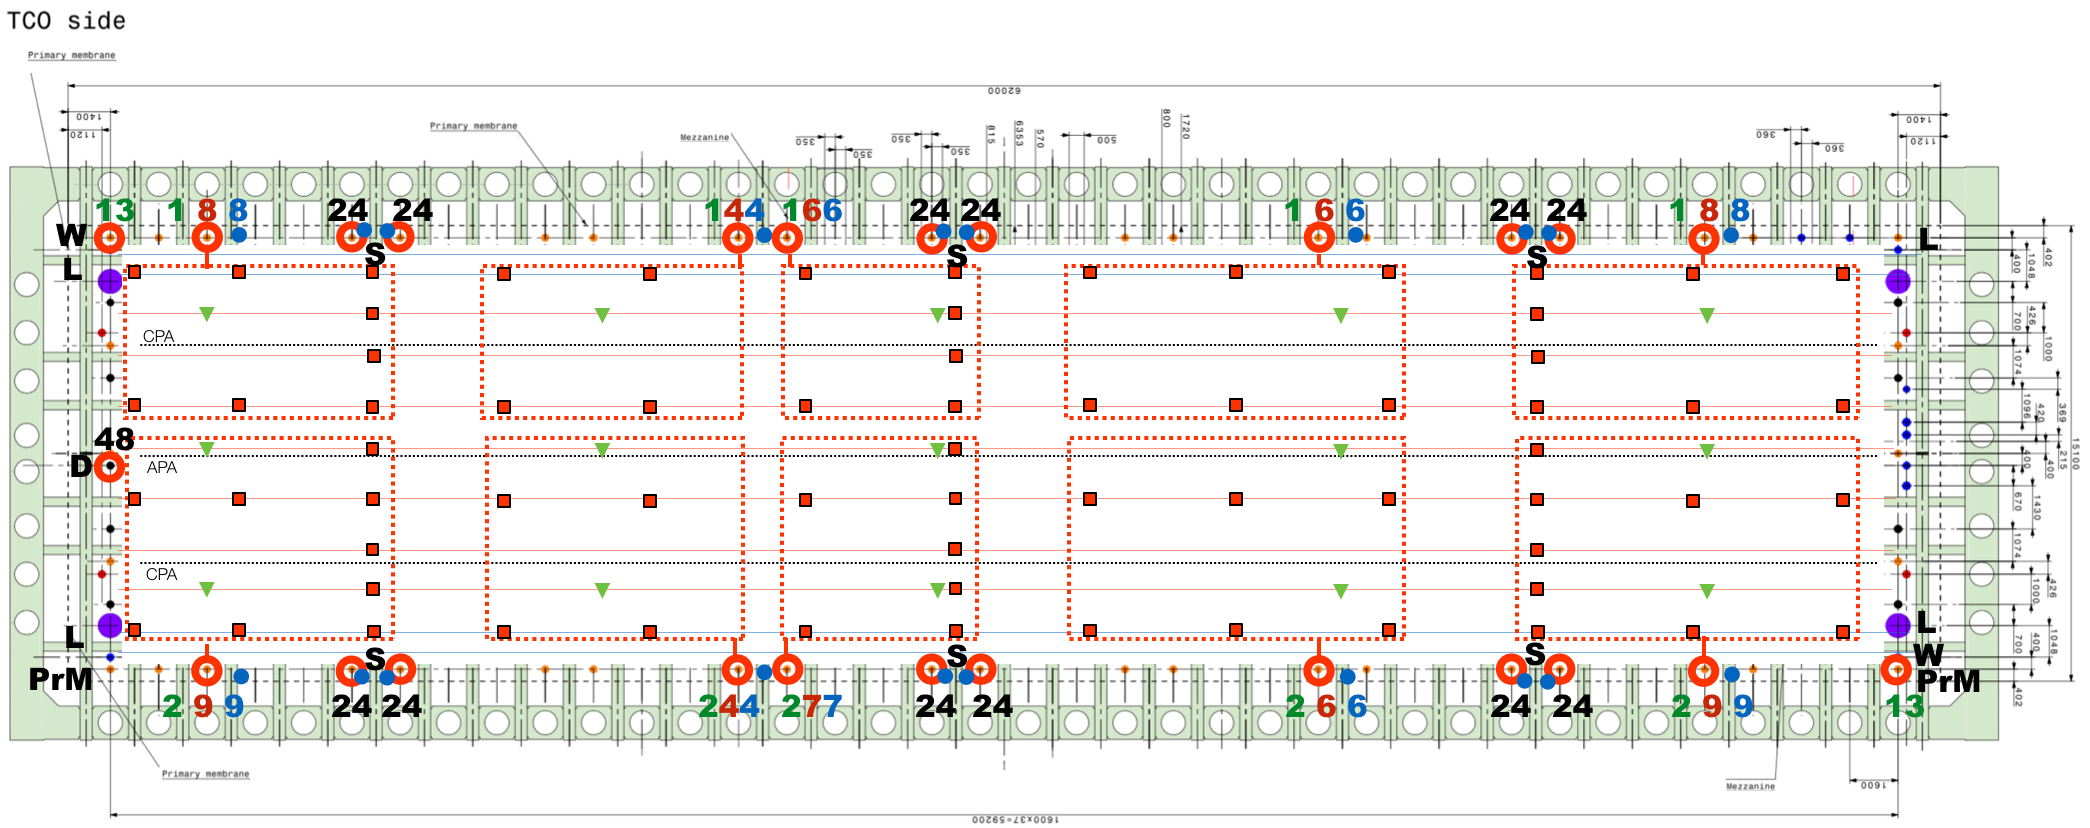
\includegraphics[width=0.98\textwidth]{cisc_distribution.png}
  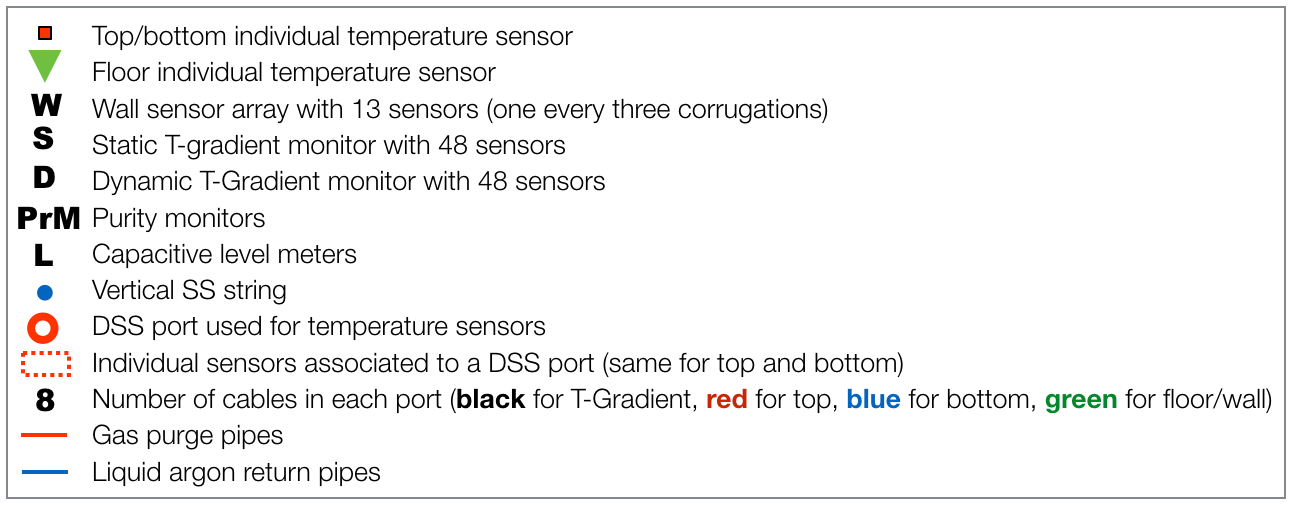
\includegraphics[width=0.85\textwidth]{cisc_distribution_legend.png}
\end{dunefigure}

\begin{dunefigure}[Endwall hoisting infrastructure]{fig:endwall-hoist}
  {Image showing the hoisting equipment used to lift the endwall into position. In this image, one of the endwalls is in place and a second is being positioned.}
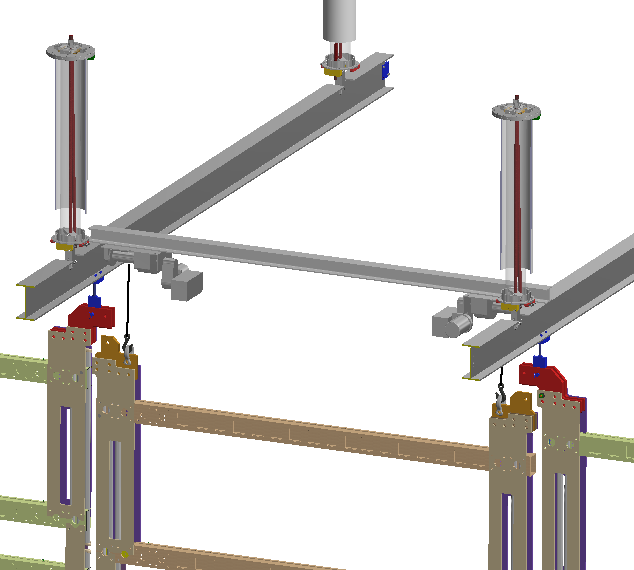
\includegraphics[width=.75\textwidth]{endwall-hoist}
\end{dunefigure}

%The next step in detector installation is installing the \dword{fc} endwall. The endwall panels will be brought underground in custom crates that fit in the cage.Each of the eight crates will hold four endwall sub-panels. Eight sub-panels are needed to build one complete 12 \si{m} tall panel.  The first step in installing the endwall is to install a custom hoist on the end of the \dword{dss} beam.This will be used to lift and assemble the sub-panels in place. The endwall transport crates will then be brought to the material airlock using a forklift. At the airlock, they are either unpacked or the crates are cleaned. Once clean, the crates are moved into the cleanroom and placed next to the \dword{tco}. Then a hoist running on the rails through the \dword{tco} is used to lift the endwalls onto the transport cart. The cart is then hoisted into the cryostat. Figure \ref{fig:endwall-cart} shows an endwall panel being transferred over to the transport cartThe top endwall sub-panel is then attached to the installation hoist and lifted out of the cart. When the sub-panel is free of  the cart, it is re-positioned so the second sub-panel can be attached to the first, and the pair is then lifted. This process is repeated until the full 12 \si{m} endwall \dword{fc} panel is assembled and can be attached to the \dword{dss}.
Next the \dword{fc} endwall is installed. The endwall panels are brought underground in custom crates. Each of the eight crates holds four endwall sub-panels. \fixme{is sub-panel a term in \dword{hv} chap? check} Eight sub-panels are needed to build one complete \SI{12}{m} tall panel.  First a custom hoist is installed on the end of the \dword{dss} beam for lifting and assembling the sub-panels in place. The endwall transport crates are then brought to the material airlock using a forklift, then cleaned.  Once clean, the crates are moved into the cleanroom and placed next to the \dword{tco}. Then a hoist running on the rails through the \dword{tco} lifts the endwalls onto the transport cart, which is then hoisted into the cryostat. Figure~\ref{fig:endwall-cart} shows an endwall sub-panel being transferred over to the transport cart. The top endwall sub-panel is then attached to the installation hoist and lifted out of the cart. When the sub-panel is free of  the cart, it is re-positioned so the second sub-panel can be attached to the first, and the pair is then lifted. This process is repeated until the full 12 \si{m} endwall \dword{fc} panel is assembled and can be attached to the \dword{dss}. 
Figure \ref{fig:endwall-hoist} shows an endwall panel being lifted into position.
All the \dword{hv} connections inside the panel can now be tested. %The process is then repeated for the remaining three endwall panels comprising the east endwall. 
While the endwall is installed, the cleanroom is configured for the installation of 
the \dword{apa}s and \dword{cpa}s. 
\fixme{check endwall vs panel vs sub-panel in pgraph above}
 
\begin{dunefigure}[Installation of the first endwall]{fig:endwall-cart}
  {The endwalls are lifted out of the transport crates using the one of the hosts on the installation switchyard. Each panel is then placed on a custom cart that is then lifted into the cleanroom.}
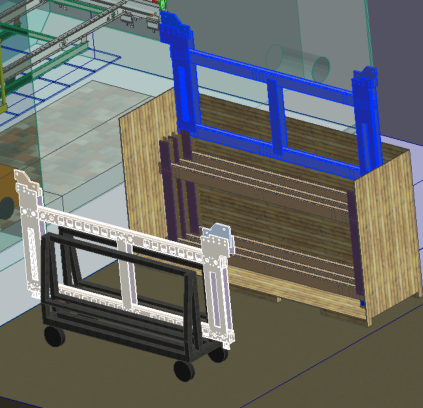
\includegraphics[width=.85\textwidth]{endwall-cart}
\end{dunefigure}


%The installation of the \dword{apa} and cathode with Top/Bottom \dword{fc} modules is the most labor intensive part of the detector installation. If possible, \dword{dune} would like to finish installing one row of the \dword{apa}, \dword{cpa}, and \dword{fc} modules every week. Figure \ref{fig:install-single-row} represents one row of the equipment. To achieve this, several separate teams must work inside the cryostat, positioning the equipment, connecting the cables, and deploying the \dwords{fc}, while  other teams work in the cleanroom assembling the equipment and performing the final cold tests. Many weeks would be needed to install a row of \dword{apa}s and \dword{cpa}s if all the work were done serially, so performing the work in parallel  as far as possible will be important for installing the equipment efficiently. 
The installation of an \dword{apa} and  \dword{cpa} with top and bottom \dword{fc} modules is the most labor-intensive part of the detector installation. Figure \ref{fig:install-single-row} represents one row of  equipment.  \dword{dune} aims to performing work in parallel to the extent possible and finish installing one row every week. This requires that several separate teams work inside the cryostat simultaneously --  positioning the equipment, connecting the cables, and deploying the \dwords{fc}, while other teams work in the cleanroom assembling the equipment and performing the final cold tests.  


\begin{dunefigure}[Single row of APA and CPA]{fig:install-single-row}
{One row of the \dword{apa} and \dword{cpa} with associated field cages is shown. In this  image, the \dwords{fc} are deployed in the final orientation. The equipment in the figure represents $1/25$ of the total TPC.}
 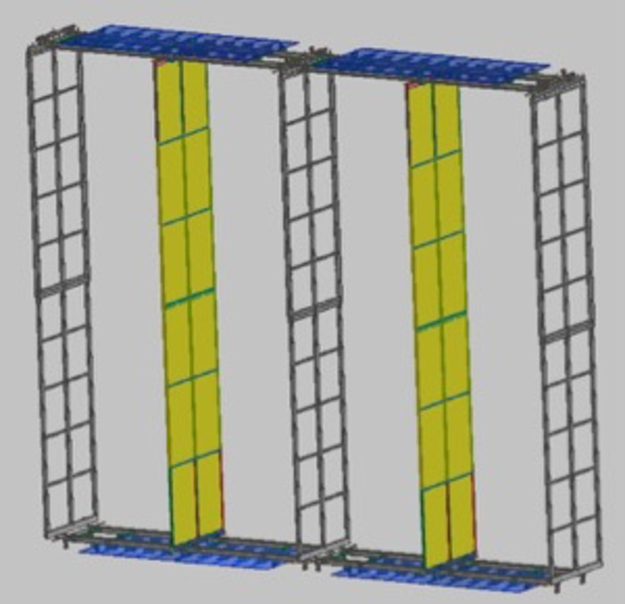
\includegraphics[width=0.5\textwidth]{install-single-row}
\end{dunefigure}

While the \dword{apa}s are installed, the area outside the cleanroom in the north cavern is available for storage; this area has sufficient capacity to store one full month's worth of equipment. 
Equipment will be brought into the cleanroom's materials airlock through a roll up door in the west wall using either an electric forklift or electric pallet jacks.  
The \dword{apa}s enter the airlock in transport crates that were used to bring the \dword{apa}s down the Ross shaft and into the north cavern. 
Each transport box holds two \dword{apa}s with associated electronics and \dwords{pd}. They enter the airlock horizontally or in a landscape orientation. 
Once inside the airlock, the dirty outer panels of the transport box are removed, a section of the roof is opened, and the bridge crane lifts the transport box to a vertical orientation. 
The airlock can then be cleaned and prepared for the \dword{apa} assembly step where the upper and lower \dword{apa} are assembled into a 12 \si{m} tall pair.
The \dword{apa} assembly sequence is shown in Figure \ref{fig:apa-assembly-v3}.

After initial visual inspection, the lower \dword{apa} is lifted out of the transport box 
using the bridge crane and mounted on the \dword{apa} assembly tower shown in green on the top row of images in in Figure \ref{fig:apa-assembly-v3}. 
The  lower \dword{apa} is supported from the bottom, and guides connected to the sides of the \dword{apa} provide mechanical stability while allowing the \dword{apa} to be lifted using jacks integrated into the lower support. A test of all the \dwords{pd} in the lower \dword{apa} is then done.  Because the cable conduit is already installed if any \dwords{pd} fail, we must remove the \dword{apa} from the tower, place it back into the shipping frame, and rotate the frame back into the landscape position.  This is the only way to remove the cable conduit. The \dword{apa} would then be loaded back into a process cart, the problem resolved, then the \dword{apa} would be placed back onto the assembly tower. 

Next, the upper \dword{apa} is lifted out of the transport box, and the transport box is removed from the airlock. The \dwords{pd} must go through the same process of testing as for the upper \dword{apa} and replaced if needed. The upper \dword{apa} is connected to the transport rail above the \dword{apa} assembly tower. At this point, the upper \dword{apa} is supported by the trolleys that move the \dword{apa}s along the transport rails, and it is stabilized using the \dword{apa} assembly frame. 
The bridge crane is no longer needed after this step, so the airlock roof can be closed allowing the air to be purified. At this time, there is a 300 \si{mm} gap between the upper and lower \dword{apa}, so now the photon cables between upper and lower \dword{apa} can be connected, and the connection from the top connectors to the SiPMs can be checked. 
To mechanically connect the two \dword{apa} modules, a metal linkage with electrical insulators is inserted into the upper \dword{apa} and bolted into place. Then the lower \dword{apa} is raised until the linkage can be bolted to the lower \dword{apa}.  
The \dword{apa} pair can then be released from the assembly tower supports and jacks; it is now supported from the top, where the upper \dword{apa} connects to the transport rail system.
After the air quality in the airlock meets the requirements for ISO-8, any dust covers are removed, and the \dword{apa} can be moved into the cleanroom through a narrow vertical door in the cleanroom wall shown in brown in the top row of images in Figure \ref{fig:apa-assembly-v3}.


\begin{dunefigure}[APA assembly steps]{fig:apa-assembly-v3}
  {Top row from left:  \dword{apa} transport crate inside the airlock; \dword{apa} transport crate rotating to vertical position;  lower \dword{apa} placed on the \dword{apa} assembly frame; and upper \dword{apa} placed on the assembly frame. Bottom row right to left: \dword{apa} pair moving on the cleanroom transport rails; \dword{apa} in  position at the cabling tower; and the \dword{apa} being inserted into the coldbox.}
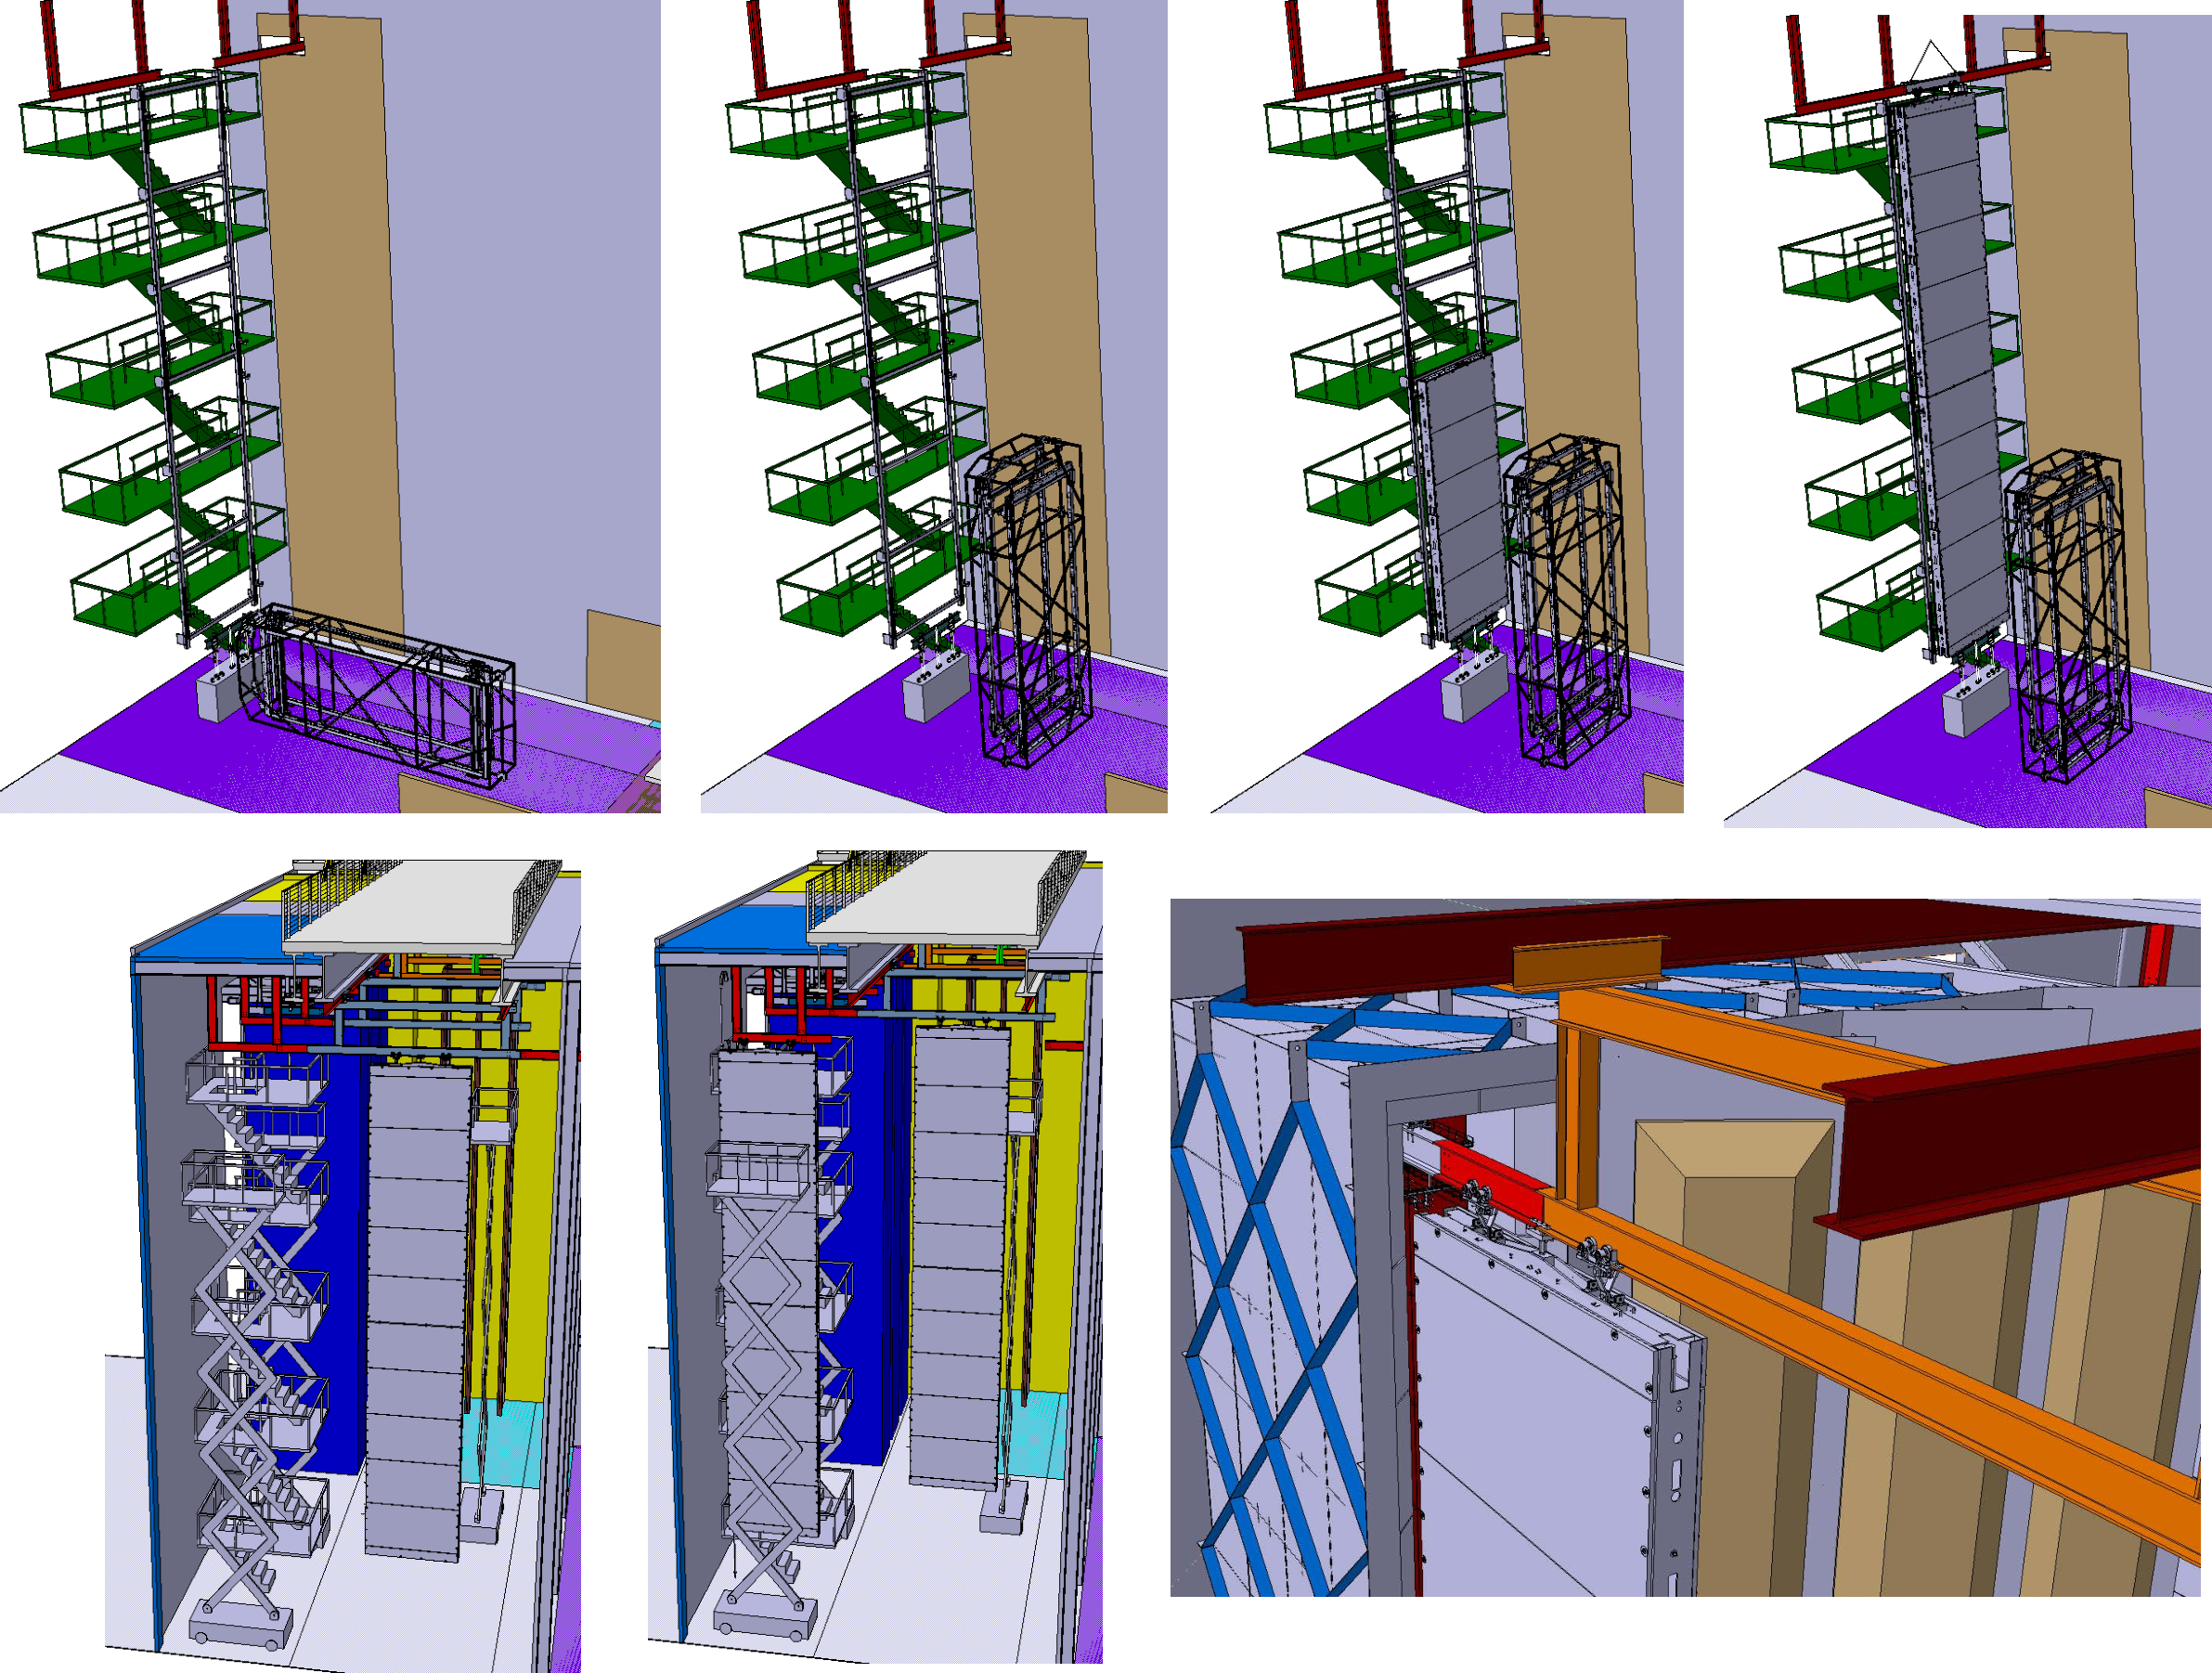
\includegraphics[width=.9\textwidth]{apa-assembly-v3}

\end{dunefigure}

The \dword{apa} pair moves onto one of the shuttle beams in the cleanroom switchyard and can be moved north-south inside the cleanroom. The next assembly step is to install and test the electronics cabling. The \dword{apa} is moved to line up with one of rails used to transport the \dword{apa}s to the \dword{apa} cabling tower. The lower left two image in Figure \ref{fig:apa-assembly-v3} shows the \dword{apa} cabling tower in the cleanroom and an \dword{apa} being moved into position. The \dword{apa} cabling tower can hold two \dword{apa} pairs simultaneously allowing one \dword{apa} pair to be cabled while a second \dword{apa} undergoes electrical testing at the same time. In this position, the cable trays and any other equipment needed during the cabling process can be installed. The electronics cables are delivered to the cleanroom on reels pre-bundled and tested. Images of the cable assembly are in the \dword{ce} section Figure XX.
\fixme{need reference from the CE section} 
The crane lifts the lower \dword{apa} reel  to the top of the \dword{apa} cabling tower, and the cable is then spooled over to a motorized deployment spool. The cable guide is then attached.  The cable guide is fed through a guide sheave and into the conduit on the side of the \dword{apa}. The cable bundle is carefully fed through the conduit and anchored in place using a cryogenic compatible cable grip. The cable is connected to the electronics at the bottom and is laid into the cable trays on top. This process is repeated for the second lower \dword{apa} cable bundle. Finally, the upper cables can be installed and prepared for transport. At this time, the functionality of all the electronics is checked. After the \dword{apa} electrical test, the \dword{apa} pair is transported to a coldbox where it undergoes a thermal cycle and complete systems test. Figure \ref{fig:apa-assembly-v3} shows the \dword{apa} being inserted into the coldbox in the lower right image. The coldbox is also a Faraday cage, so noise levels can be measured and the photon system checked for photon sensitivity. After the cold test is complete, an \dword{apa} will either move back to the cabling station if any repair is needed, or it will be moved into the cryostat for installation. 



\begin{dunefigure}[CPA assembly steps]{fig:install-cpa-assembly}
  {The \dword{cpa} assembly steps are shown. Top row from left:  \dwords{cpa} are delivered to the CPA assembly fixture in the cleanroom; the 3 \si{m} sub-panels are lifted onto the frame and connected. Bottom row from left: After the CPA panel is complete, it is moved into the room and the field cage modules are attached. The CPA is then moved into the cryostat.}
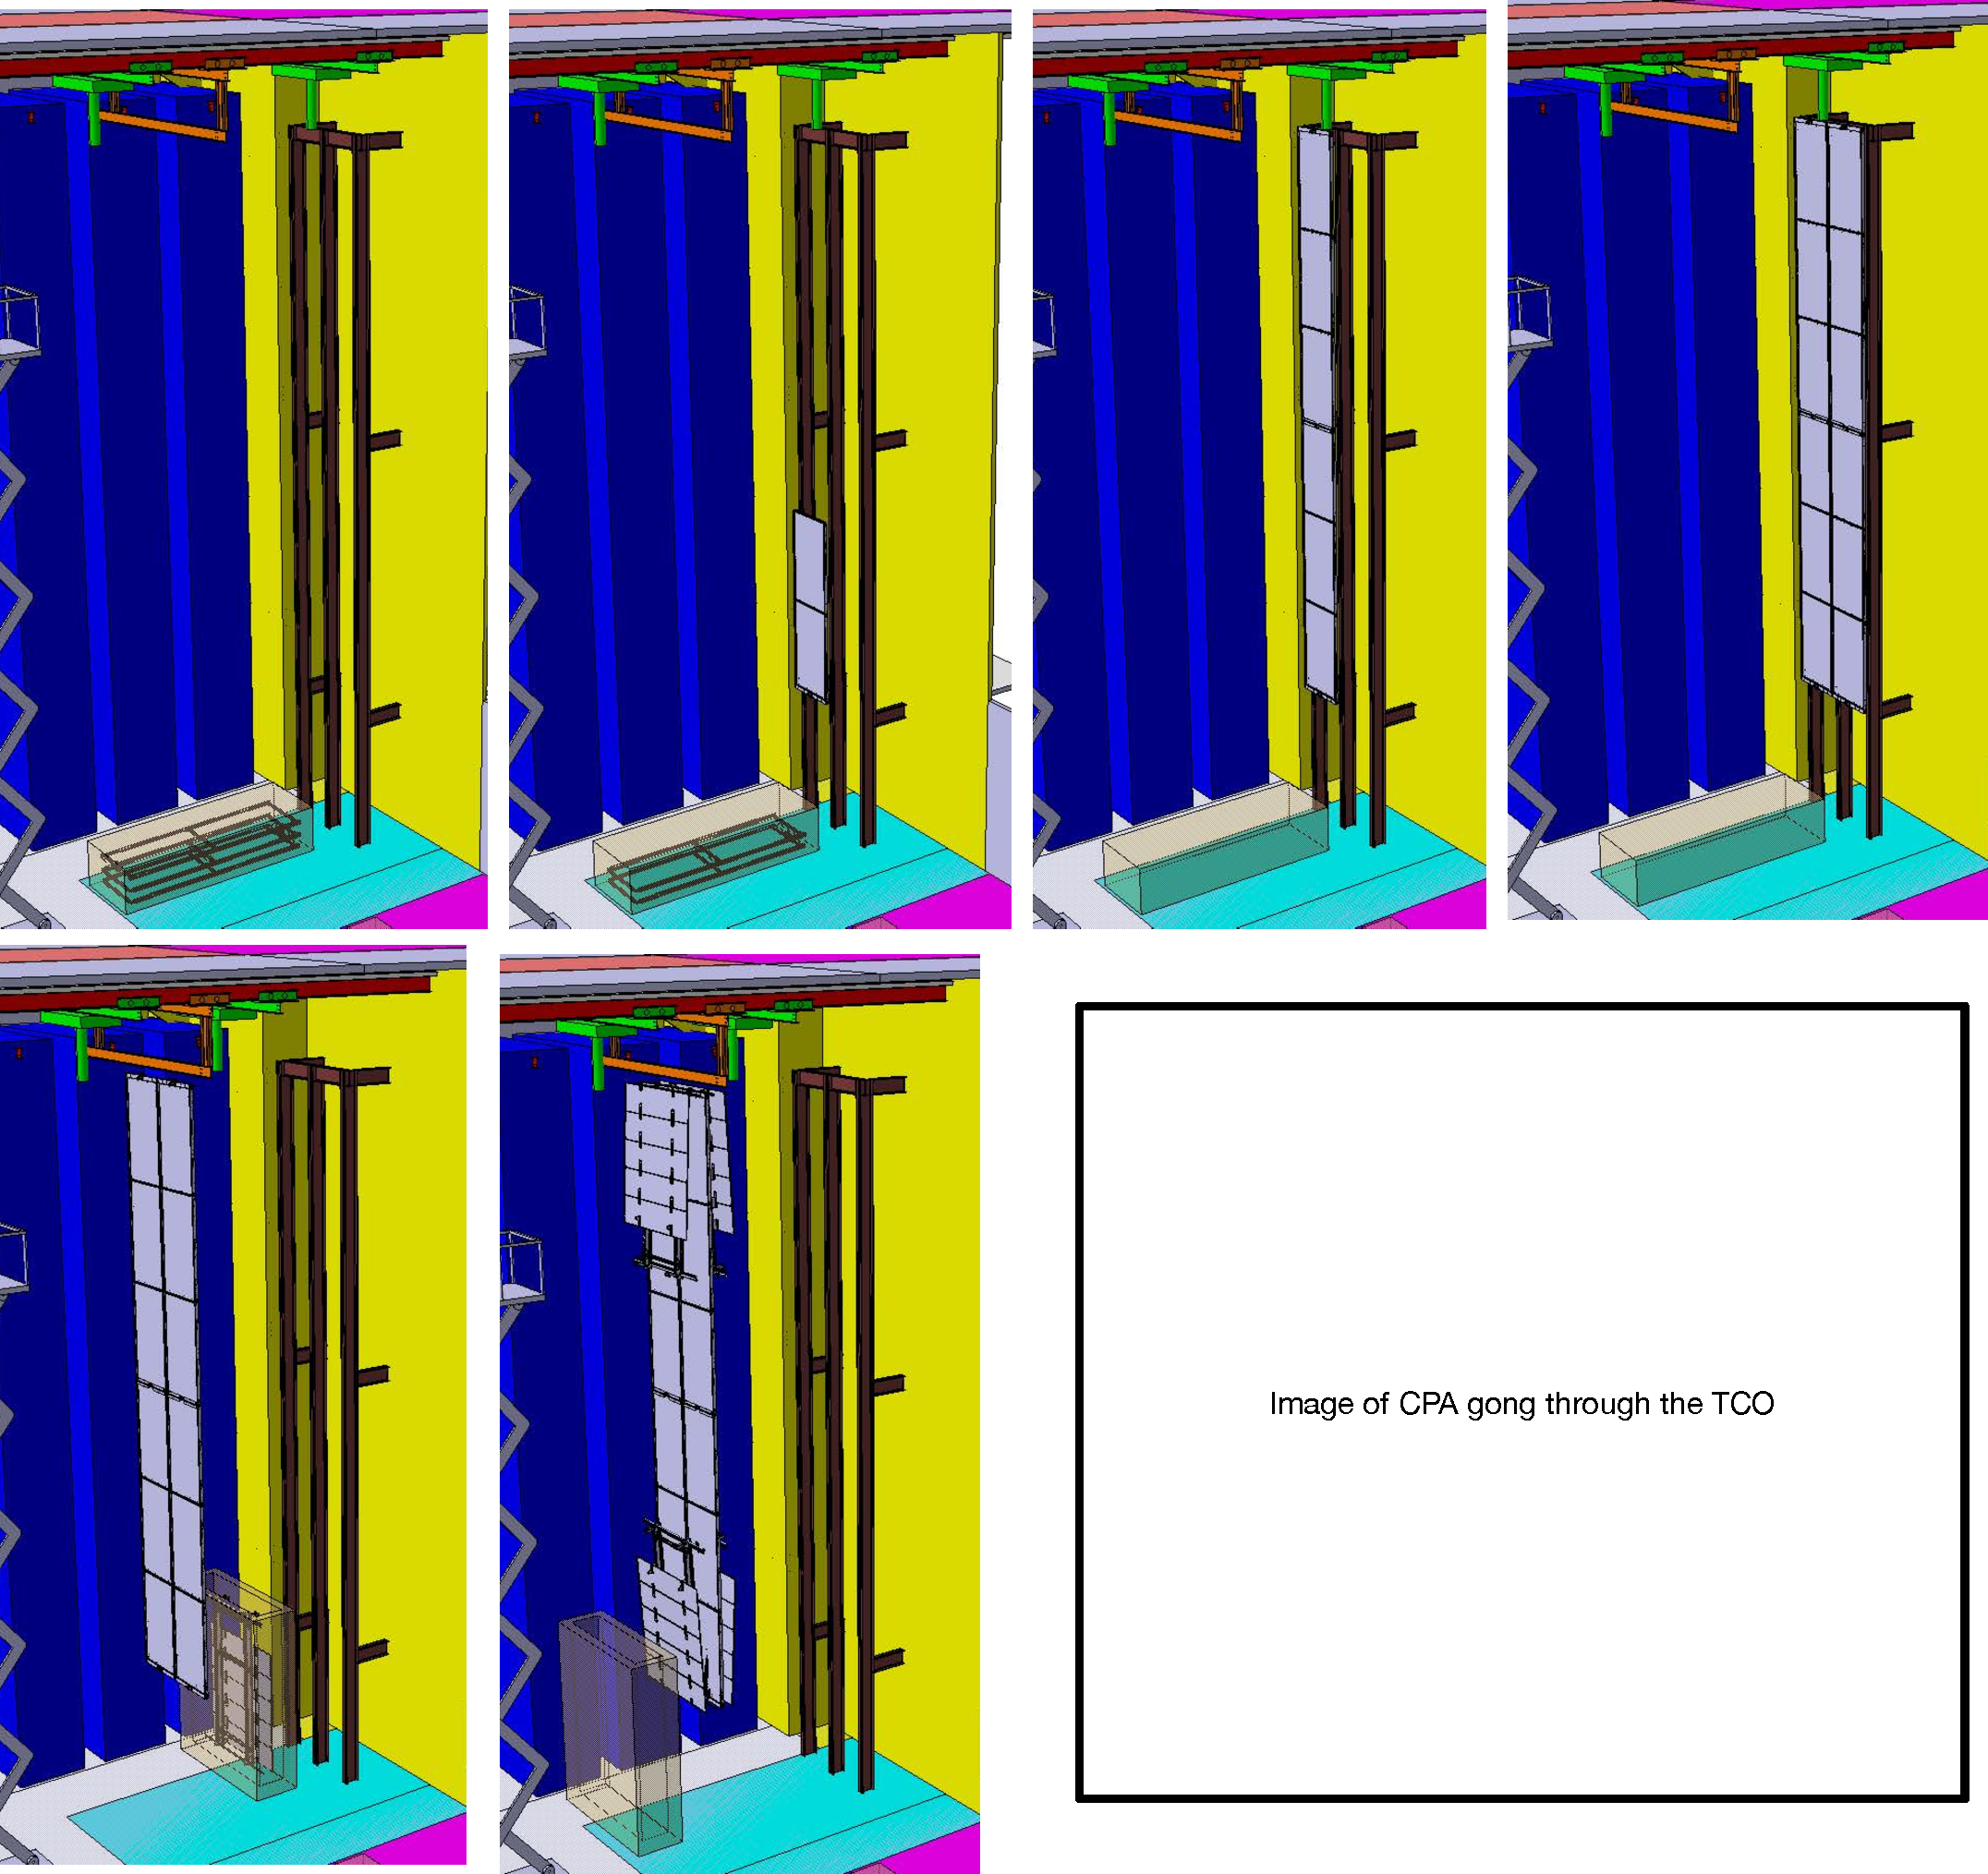
\includegraphics[width=.9\textwidth]{install-cpa-assemble}
\end{dunefigure}

The CPA and top \dword{fc} modules are assembled in parallel to the \dword{apa} assembly. Figure \ref{fig:install-cpa-assembly} shows the  assembly sequence. The sub-panels for the cathode plane are delivered to the airlock in crates that hold 4 \si{m} long 1.15 \si{m} wide segments. After cleaning, the crates are brought into the cleanroom and opened. The panels inside are bagged to provide additional dust protection. The sub-panels are lifted out of the crate and placed on the assembly frame using the cleanroom switchyard hoist. First one of the 1.15 \si{m} 4 
\si{m} tall sections is assembled, followed by the second and third ones. The 1.15 \si{m} wide section is then lifted, connected to the installation switchyard, and moved to the \dword{tco} beam. The second 12 \si{m} tall section is then assembled like the first. The two 1.15m wide panels are then connected to make the 2.3 \si{m} wide unit.  A complete set of \dword{qc} measurements are taken of all electrical connections between panels.  The cathode assembly  is then moved to a location in the switchyard where the diffuser fibers and top field cage modules can be installed.
 The top \dword{fc} modules are then attached. In Figure \ref{fig:install-cpa-assembly}, the completed assembly is shown with the lower \dword{fc} modules also attached. This is an option, but present planning is to install the lower \dword{fc} modules  inside the cryostat. Finally, the \dword{cpa}-\dword{fc} assembly is moved into the cryostat.


\dword{pd} monitoring system optical diffusers and short optical fibers must be connecetd to the \dword{cpa} panels before the panels are installed in the cryostat.  Discussions are underway about the optimal site for this installation:  at the \dword{cpa} assembly facility before shipping to the site, or as part of the assembly of \dword{cpa} stacks in the underground cleanroom.  Whichever solution is adopted, quartz optical fibers must be routed from the diffuser to the top of the \dword{cpa} assembly to be connected later to the pre-installed fibers in the cryostat; this connection will occur upon final positioning of the \dword{cpa}.  

Work inside the cryostat will proceed in parallel with the work in the outer cleanroom. 
The large detector components like \dword{apa} pairs and \dword{cpa} modules will enter the cryostat using the \dword{tco} rails that connect to the \dword{dss} switchyard.
Inside the cryostat, the modules will be pushed onto one of the switchyard shuttle beams shown in  Figure \ref{fig:shuttle}. 
The \dword{dss} shuttle beam is then moved to the appropriate row of the \dword{dss}, and then the module is pushed down the length of the cryostat into position. The position of the \dword{dss} beams are well defined and accurately surveyed so the \dword{apa} and \dword{cpa} modules can be accurately located by precisely positioning them along the \dword{dss} beams. A small correction in the height of the modules may be needed to accommodate deflections in the \dword{dss} due to load. Figure \ref{fig:install-ce-cables} shows the typical situation during the \dword{apa} installation and \dword{ce} cabling. 

\begin{dunefigure}[Cold Electronics cabling inside the cryostat]{fig:install-ce-cables}
  {The installation of the APA and cabling of the cold electronics is described. The left panel shows the APA installation process. One row of APA and \dword{hv} equipment is installed, and a second APA is ready for electrical cabling. The top right image shows the cable trays that will hold the CE cables; one worker is in the scissor lift. The left bottom image shows the work space with the geometry of the APA, the cryostat roof, and the cable feedthrough.}
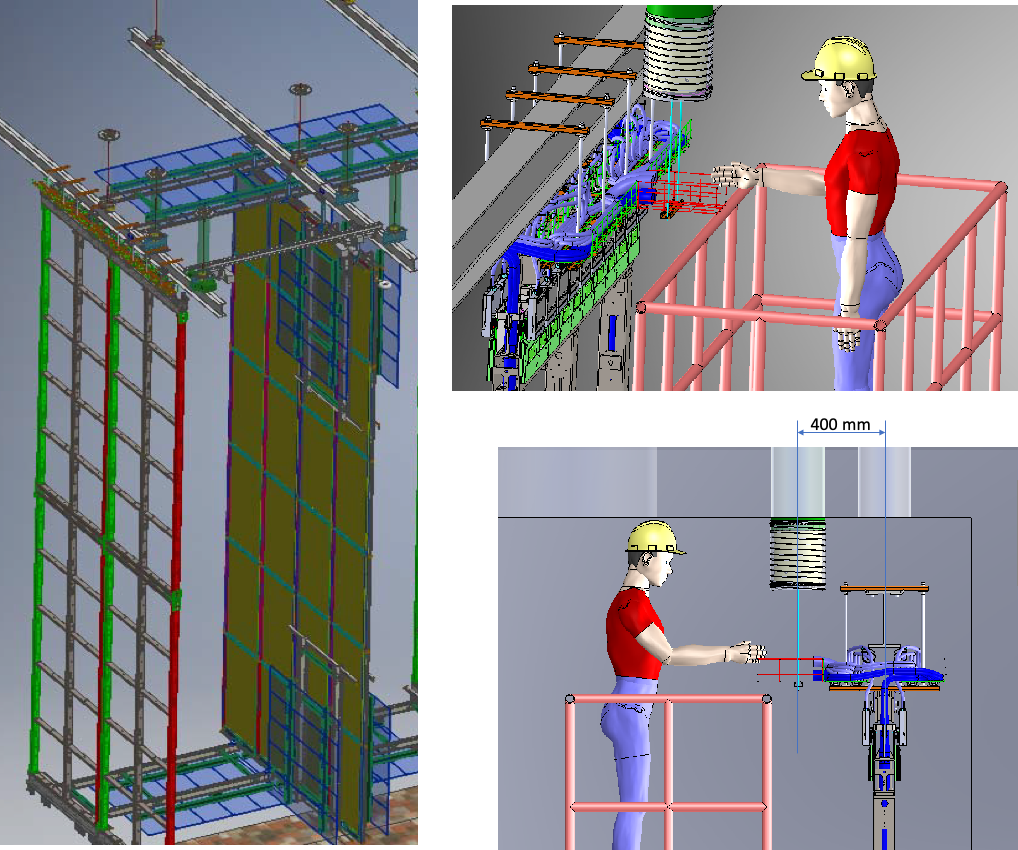
\includegraphics[width=.9\textwidth]{install-ce-cables}
\end{dunefigure}

After the \dword{apa} is moved into position, the permanent support rod is connected to the \dword{dss} beam, and the trolleys are removed. 
The crawler used to push the \dword{apa} along the rails is then moved back through the shuttle area and can be used for the next module. 
After the \dword{apa} is locked into position, the cable tray feedthrough to the \dword{ce} is installed. Now \dword{ce} cabling can start. 
Even when a \dword{cpa} module is already in position, more than 3 \si{m} space remains free between the \dword{apa} and \dword{cpa}, so a scissor lift can easily be positioned in front of the \dword{apa}. 
The two right images in Figure \ref{fig:install-ce-cables} show the situation at the top of the cryostat during cabling. The cables are not shown, so the cable trays and their support infrastructure can be seen. 

When cabling begins, all the cables are in the cable trays. 
A team of two people are in the scissor lift in front of the \dword{apa}, and another team of two people are on top of the cryostat. 
The \dword{ce} cables from the bottom \dword{apa} emerge from the \dword{apa} side-tube and are split into two bundles in the cable tray for a total of four cable bundles. 
The top \dword{apa} also has \dword{ce} cables organized into four bundles. 
The photon cables from both the top and bottom \dword{apa}s are bundled into two cable bundles.
During the cabling process, each bundle is partly removed from the cable tray and then fed up through the cable feedthrough. 
At the top of the feedthrough, the cables are strain relieved, and the cables are also strain relieved at the bottom of the crossing tube.
This is repeated for each of the 10 cable bundles needed for the \dword{apa} pair. 
When all cables are installed through the cable tray, any excess length is returned to the cable tray at the top of the \dword{apa}. 
On the roof, the short individual cables are then connected to the feedthrough flange, and the electronics can be tested. When all electronics and electrical connections are checked, the flange connecting the warm interface crate can be sealed to the cryostat feedthrough flange, and the cable installation is complete. 

Similarly, the \dword{pd} warm cables are connected to the readout module, and the flange sealed after testing.  Once testing is complete, the tray holding the excess cabling is transferred to the \dword{dss} beam.  This minimizes any uneven load on the \dword{apa} pair, so they hang more vertically.   
The electronics for each \dword{apa} is continuously monitored after installation. 

Placing the cables in the cable trays and exactly how the cables are routed is complex. Figure \ref{fig:install-cable-routing} shows the working 3-D model of the cable routing, showing how the cables will be bundled and placed in the trays. A mock up the cabling configuration is planned at BNL, and the installation of the cables will be tested as part of the Ash River testing program.

\begin{dunefigure}[Model of the electronics and photon detector cabling]{fig:install-cable-routing}
  {Working model of the cable trays and routing of the cables in the trays.}
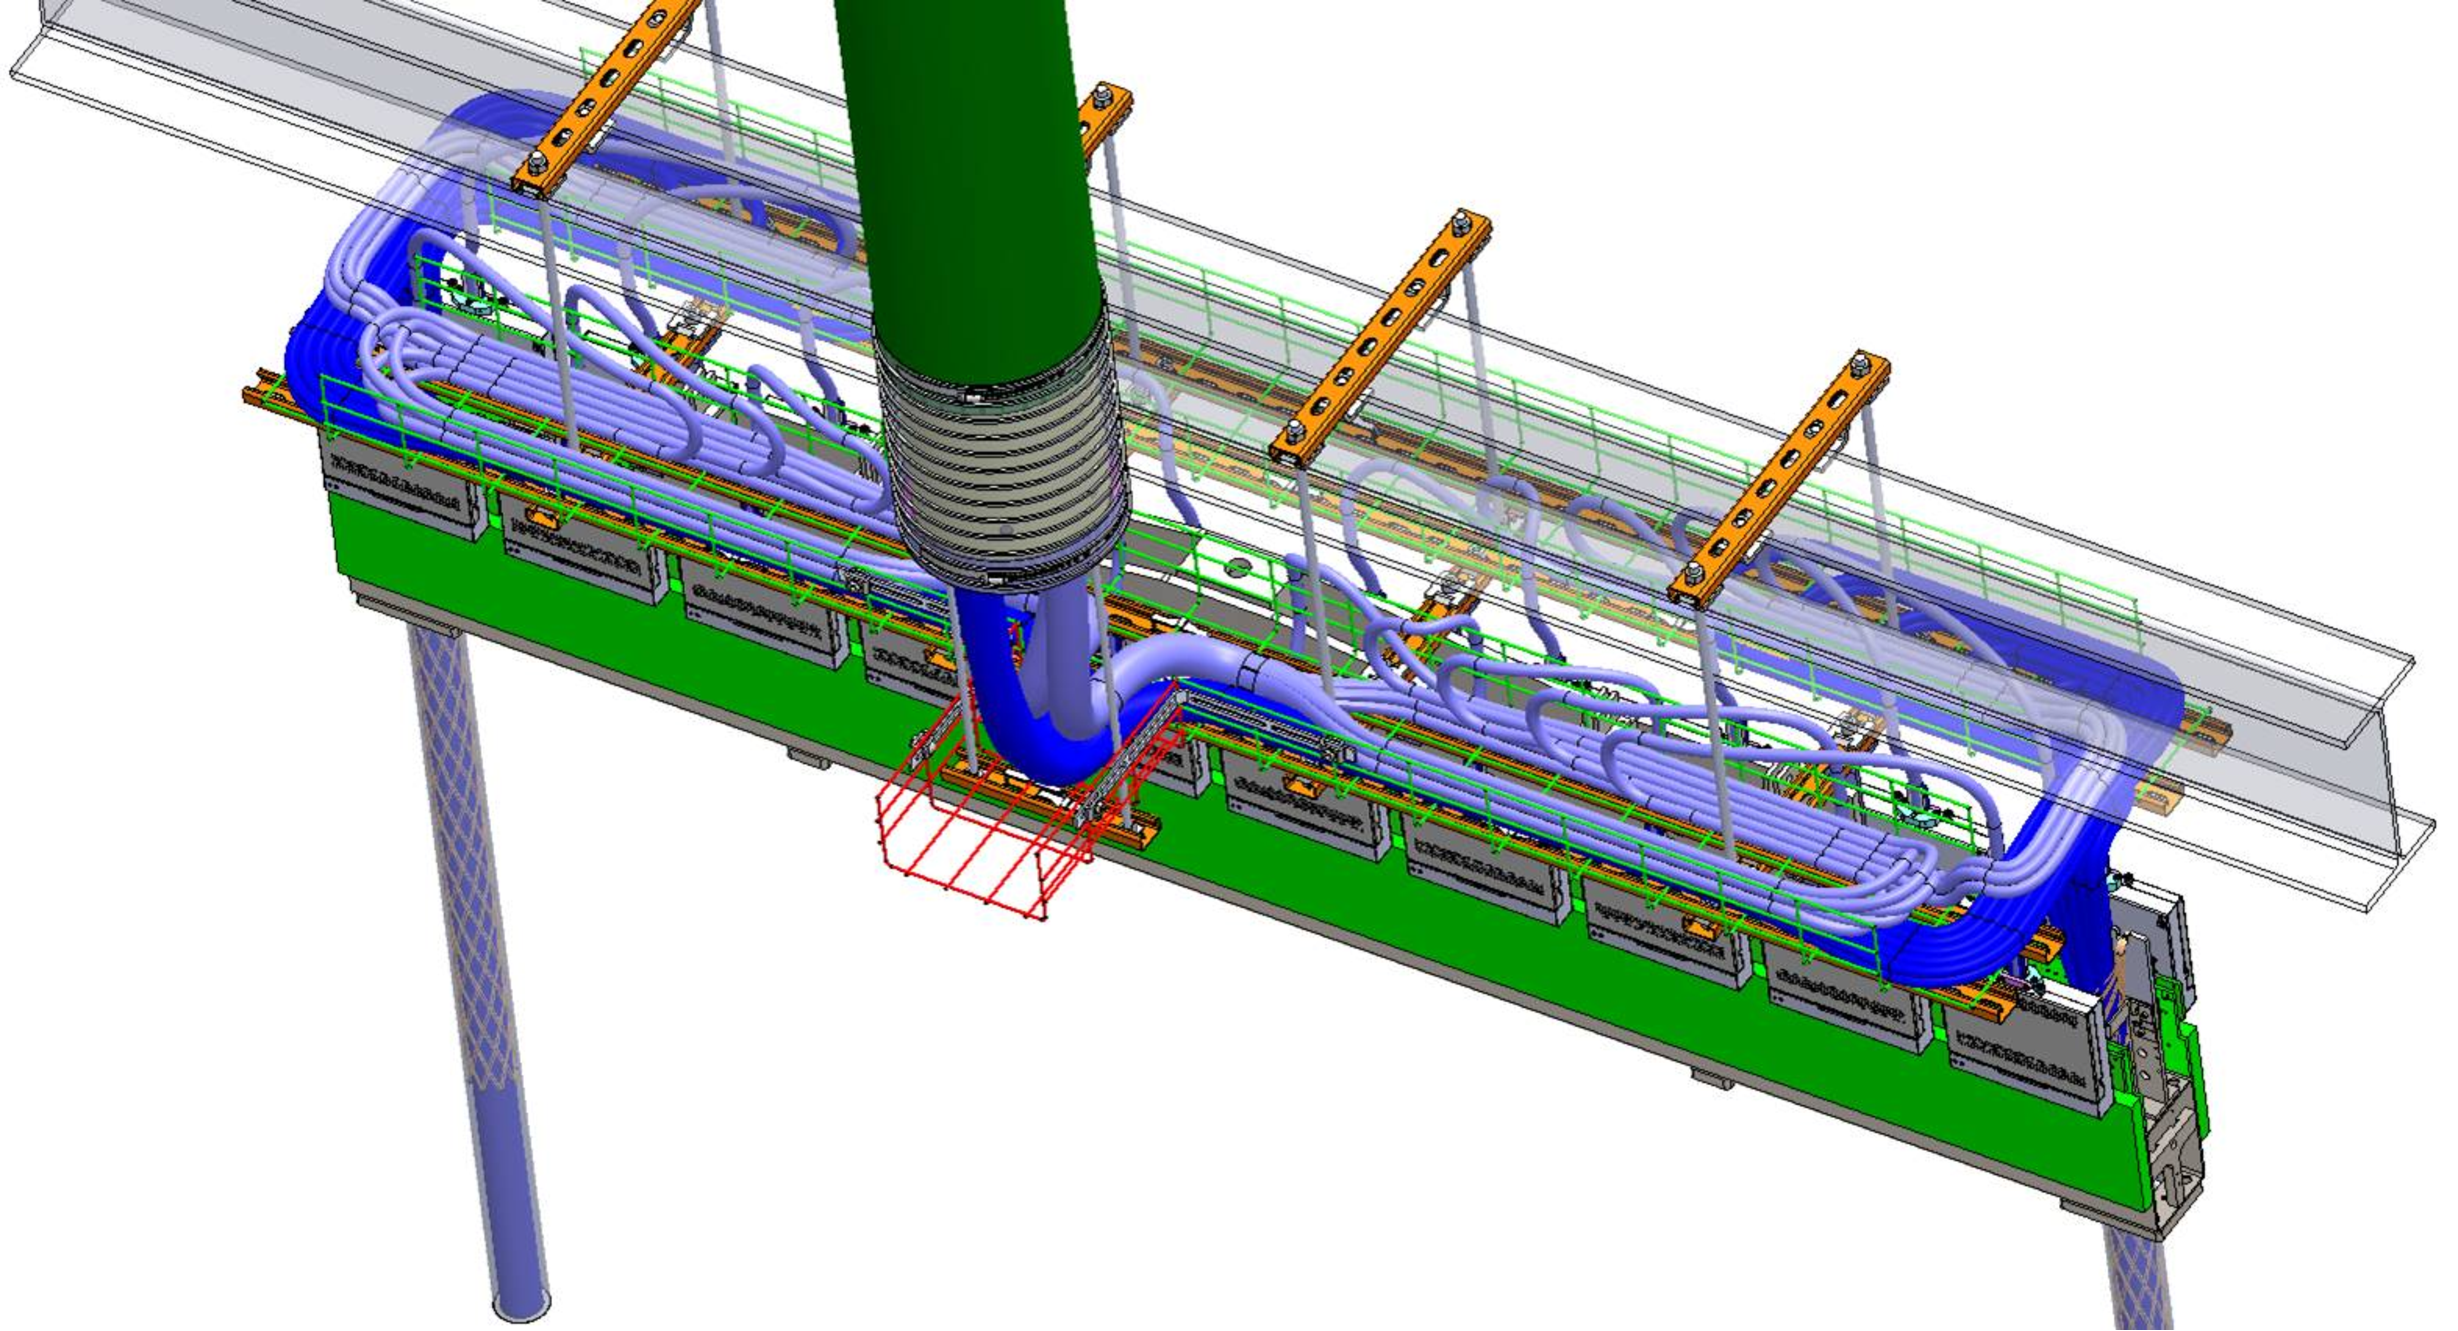
\includegraphics[width=.95\textwidth]{install-cable-routing}
\end{dunefigure}


\begin{dunefigure}[CPA installation]{fig:install-cpa-fieldcage}
  {The top field-cage assemblies are deployed using a custom tool that mounts to the DSS beams as seen in the top left panel. The field cage is lifted using the electric winch controlled by an operator in the nearby scissor lift. The lower field cage is lowered using a hoist mounted on a wheeled frame. The hoist is on a linear slide to keep it aligned above the connection point.}
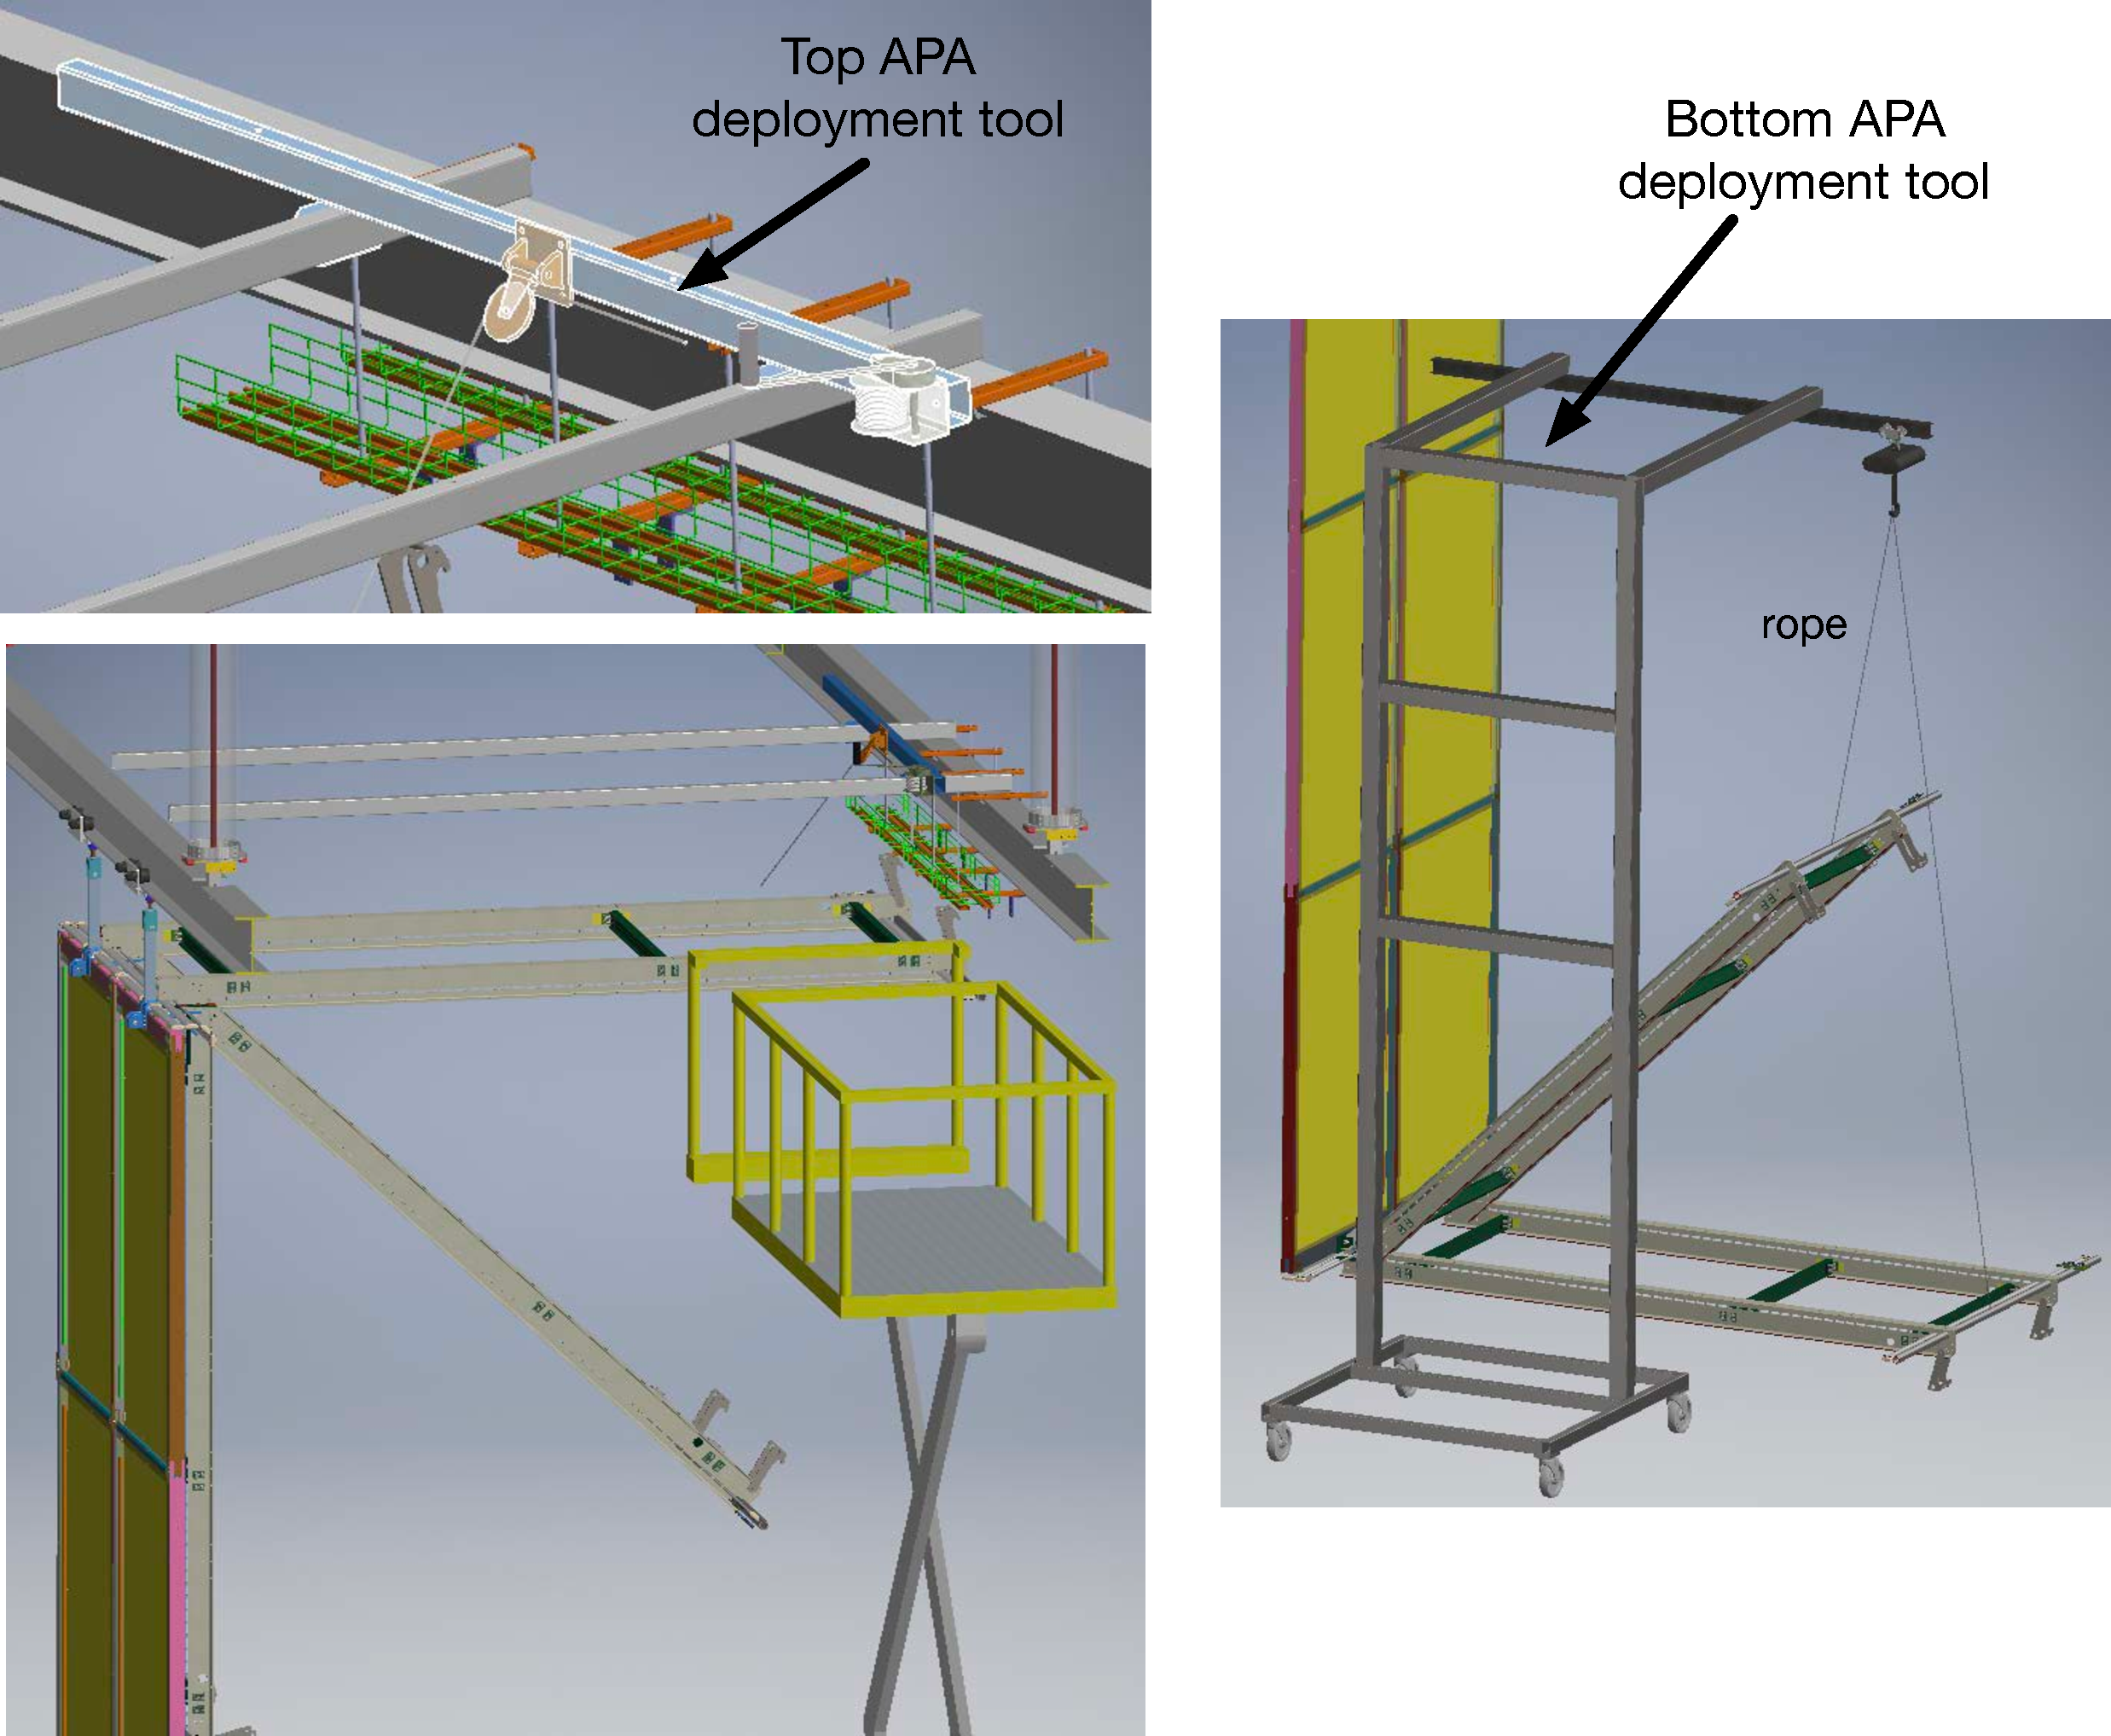
\includegraphics[width=.9\textwidth]{install-cpa-fieldcage}
\end{dunefigure}

The cathode \dword{fc} assemblies are brought into the cryostat like the \dword{apa} pairs, using the overhead rails through the \dword{tco}. Inside the cryostat, they are moved into position using the \dword{dss} switchyard and \dword{dss} I-beams. 
Once in position, the load is transferred to the \dword{dss} beam, and the trolleys are removed. 
The \dword{cpa} will wait in position until its \dword{apa} pairs are fully tested, and then the \dword{fc} modules could be deployed. 
The deployment sequence of the \dword{fc} has not yet been fixed. 
If the \dword{fc} are immediately deployed then the \dword{apa} and \dword{fc} can be tested in the final position. 
If one waits to deploy the field cages then the \dword{ce} can undergo a longer burn in test and the opportunity to clean the cryostat near the end of the installation is available. The decision on the best time to deploy the \dword{fc} will be made closer to the start of installation.
Figure \ref{fig:install-cpa-fieldcage} shows the equipment for deploying the \dwords{fc}. 
The top \dwords{fc} are raised by connecting a cable to the module and then using a pulley-winch assembly to lift the module, which latches to the \dword{apa} mounts. 
A scissor lift is used to connect the cable to the module and also to control the winch. 
After the module is in place, the deployment tool is moved to the next \dword{apa}and \dword{cpa} sets. 
The lower \dword{fc} is deployed using a custom frame that can be wheeled into position. 
The cable from a small host is then attached to the \dword{fc} module, and the module can be lowered. 
The hoist is on a linear slide, so the cable is always directly over the connection point. 
This keeps the \dword{cpa} from swinging because of an induced moment. 
When the module is down, it latches to the \dword{apa} frame much like the upper \dword{fc}. 
The electrical connections to the \dword{hv} bus are tested, and deployment is complete. 
In principal, the cathode/\dword{fc} assemblies can be constructed faster than the \dword{apa}s. 
In theory the cathode/\dword{fc} assembly process could start later than the start of \dword{apa} assembly if the deployment is postponed. 
 The risks and benefits of different deployment sequences will be evaluated near the start of installation.

The periscopes for the laser calibration system on the top of the TPC in the center can be installed after the relevant \dword{fc} elements are deployed. The lasers are immediatedly aligned with the alignment laser system. 
Once for each periscope/laser system, prior to the installation of further TPC components, we will need to clear the cavern to align the UV (Class 4) and visible lasers this will need special safety precautions. 
It may be possible to do this special alignment operation for all lasers at roughly the same time, to minimize the disruption.

\begin{dunefigure}[Installation of row 25]{fig:install-row25}
  {Detector installation as the last row of detector components are installed. At this time, the switchyard beams are removed, and the temporary hoists for the endwall are installed.}
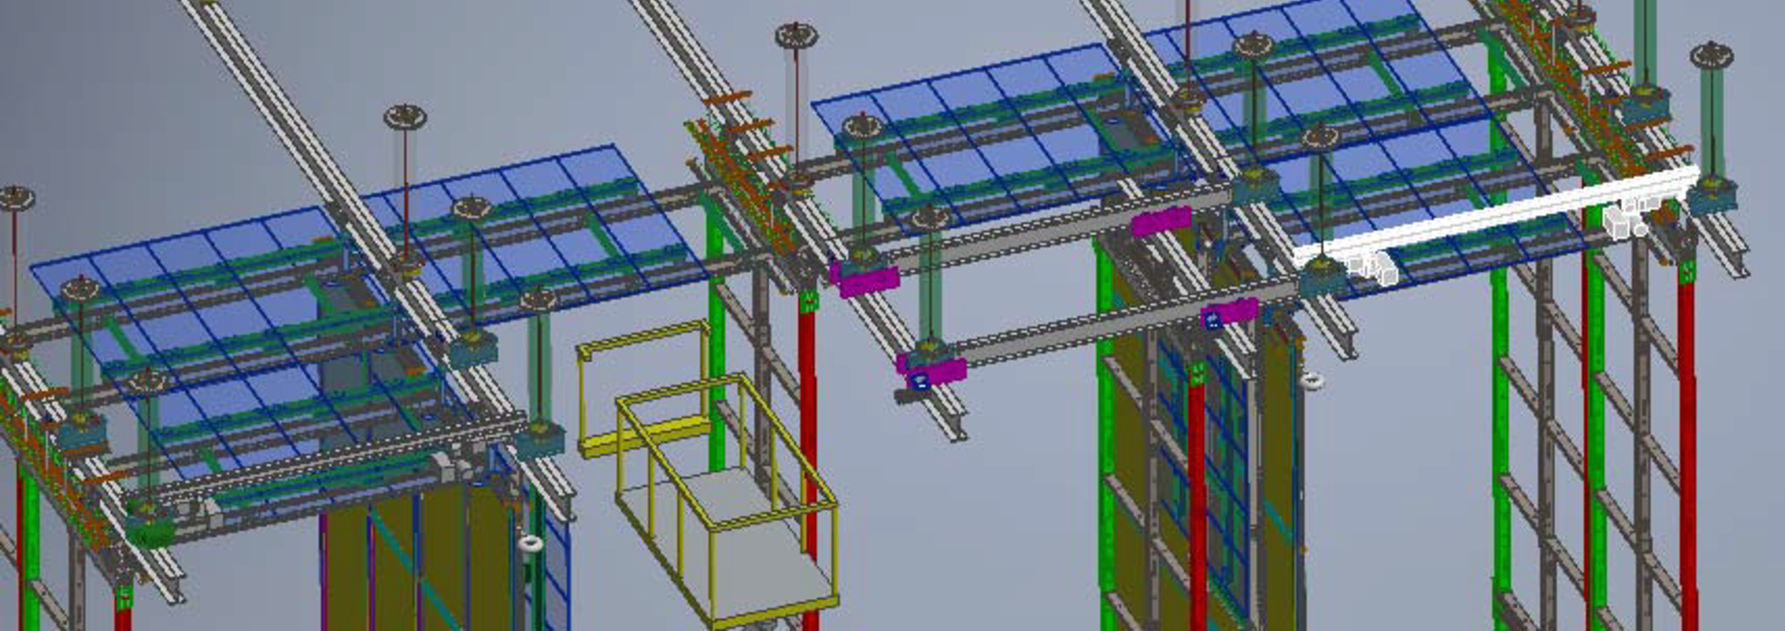
\includegraphics[width=.9\textwidth]{install-row25}
\end{dunefigure}


The last row of detector elements are installed much like previous rows, but the runway beams of the \dword{dss} switchyard are removed as this \dword{apa} and \dword{cpa} are placed in position. Figure \ref{fig:install-row25} shows the top of the detector as this last row is installed. When the shuttle beam is aligned to the correct \dword{apa} or \dword{cpa} row, the short section of the beam is bolted to a short I-beam section of the runway beam that is permanently fixed to the \dword{dss} support feedthrough. When the shuttle beams at both ends of a runway beam section are fixed in position, a section of the runway beam is removed. The last \dword{fc} modules are then deployed. 


\begin{dunefigure}[Second endwall installation]{fig:install-ew2}
  {Installation of the final endwall before closing the TCO.}
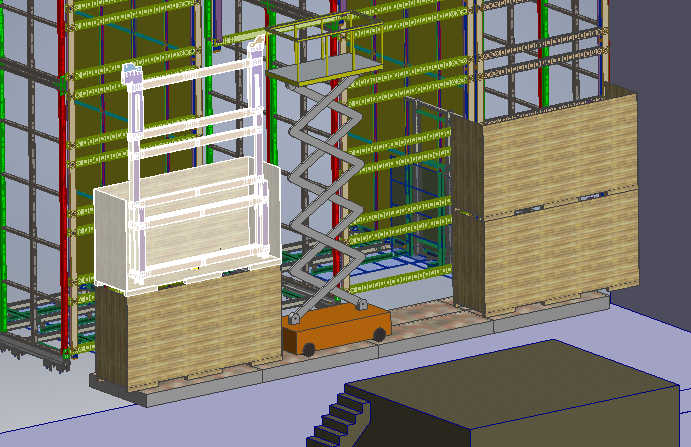
\includegraphics[width=.9\textwidth]{install-ew2}
\end{dunefigure}

The second outside endwall is installed like the first endwall. At this point, the center \dword{apa} is rolled into the cryostat, the shuttle beam is bolted to the \dword{dss}, and the runway beams are removed. The two center drift volumes \dwords{fc} are deployed. The last two endwalls are constructed, and the \dword{tpc} is basically finished. 

At this point, a frame supported by the shuttle beams is covered with flame retardant plastic and installed to create cleanroom work area for the \dword{tco}.  A scaffold is set up for egress to the manhole. The cryostat will become confined space area, so it must be in place before the \dword{tco} is closed.  Closing the top 3/4 of the \dword{tco} is completed using the 14m scissor lift. The temporary cleanroom area is then removed and the area cleaned. A smaller clean area is made to cover the bottom 3.4m \dword{tco} section.  The scissor lift must be removed at this point. The \dword{tco} work is completed and the area cleaned.

A second scaffold is set up in this space  for cleaning and installation of equipment for the calibration and cryogenic instrumentation.

The dynamic T-gradient monitor is installed at this time. 
The monitor comes in several segments with pre-attached sensors and cabling already in place. Each segment is fed into the flange one at a time until the entire sensor carrier rod is in place. The remainder of the system (motor system that moves the sensor rod and the sensors) that goes on top of the flange is installed using a crane. 

The purity monitor system will be built in modules, so it can be assembled outside the cryostat leaving only a few steps to complete inside the cryostat. 
The assembly itself comes into the cryostat with the three individual purity monitors mounted to support tubes that are then mounted to the brackets inside the cryostat. The brackets are then attached to the appropriate elements (cables trays, \dword{dss}, and bolts in the cryostat corner are under consideration). Also at this time, the remaining level monitors are installed.

The periscopes at the end of the detector are installed and aligned. 

Once all this work is completed, the scaffolding is taken apart and hoisted out the man-hole along with all remaining flooring sections. The area is cleaned, and the last two \dword{fte} in the cryostat are hoisted out. 

The inspection cameras and other possible calibration instruments can be installed from the roof while the \dword{tco} is being closed.

After the TCO is closed the manholes can be closed and the pulsed neutron source can be placed in position above two of the manholes. The pulsed neutron source can be tested to confirm neutron yields with integrated monitors and dosimeters in dedicated runs..

% clear the figure buffer before starting the next section
%\clearpage




%%%%%%%%%%%%%%%%%%%%%%%%%%%%
\subsection{Prototyping and Testing (QA/QC)}
\label{sec:fdsp-tc-inst-qaqc}

The experience gained during the \dword{protodune} Ash River trial assembly was critical for both verifying the mechanical design and interface but also tor developing the tools and procedures needed for the installation.
Testing access using a fake cryostat roof or walls was important to understanding how some tasks could physically be performed. 
\dword{dune} will have half the available work space inside the cryostat both the above and below the \dword{tpc}.  One lesson learned from \dword{protodune} was that access was difficult in this area as we secured the bottom latches and tied the \dword{apa}s together on the bottom.  The process of developing hazard analysis and procedure documentation for the assembly process is important to gain approval to begin installation.   

Mechanical tests at the \dword{dune} trial assembly at Ash River are key to developing the installation process, but other important prototyping tasks are done at other universities, national laboratories, and CERN also are needed to develop the installation plan. Argonne National Laboratory is testing the \dword{apa} shuttle beam drive system and the \dword{cpa} assembly tower connections before they are shipped to Ash River.  
Darnsbury has constructed new process carts using the lessons learned from \dword{protodune} to make the assembly tasks both more efficient and safer. 
Many small steps in the assembly process have been improved using our past experience at CERN and will be developed further during this prototyping phase. 

The different consortia are responsible for developing the \dword{qc} program for their deliverables during the installation phase. 
The program is further described in the following \dword{qc} sections. First the Ash River tests will be described then the \dword{qc} for the consortia deliverables.

\subsubsection{Ash River Testing}

Full scale mechanical testing of the assembly and installation of all the \dword{tpc} components, including the \dword{dss}, will be critical for the success of the single phase detector as shown from the \dword{protodune} prototyping experience. 
The \nova Far Detector assembly area at Ash River, shown in Figure \ref{fig:NOvA-Assembly-Area}, meets the criteria of both area and available equipment as well as having experienced technicians that helped construct the \dword{protodune} detector. 
By definition, the installation  is on the critical path, making it vital that the work be performed efficiently and with low risk. 
To achieve this, a prototype of the installation
equipment for the \dword{spmod}  will be constructed at Ash River (the \nova neutrino experiment \dword{fd} site in Ash River, Minnesota, USA), and the installation process tested with dummy detector elements.  
Just before beginning installation then, the Ash River set up will be used as a training ground for the installation team. 

\begin{dunefigure}[NOvA Assembly Area at Ash River]
{fig:NOvA-Assembly-Area}
{Top Panel shows the NOvA Assembly Area and the bottom panel shows the 3-D model of the installation prototype.}                
%\centering     %trim=left bottom right top, clip
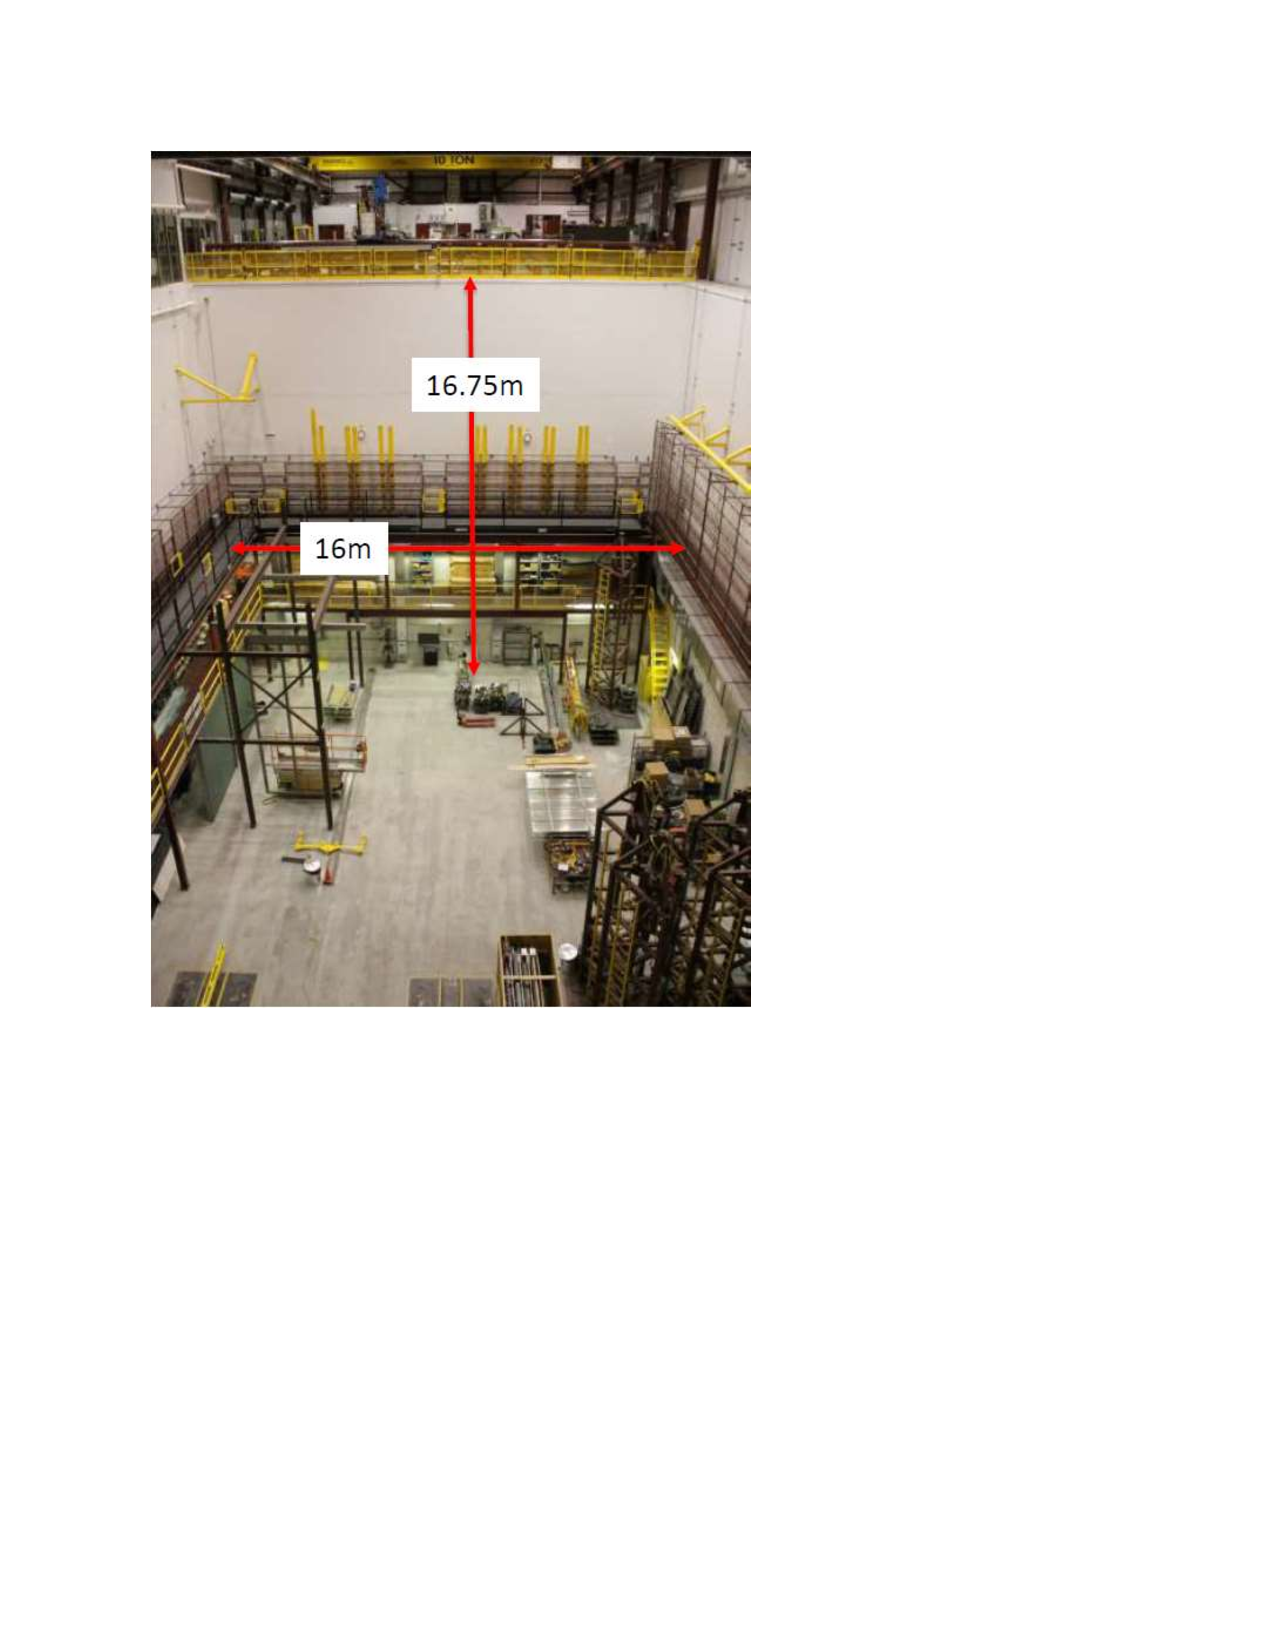
\includegraphics[width=0.49\textwidth]{NOvA-Assembly-Area}
\vspace{-12pt}
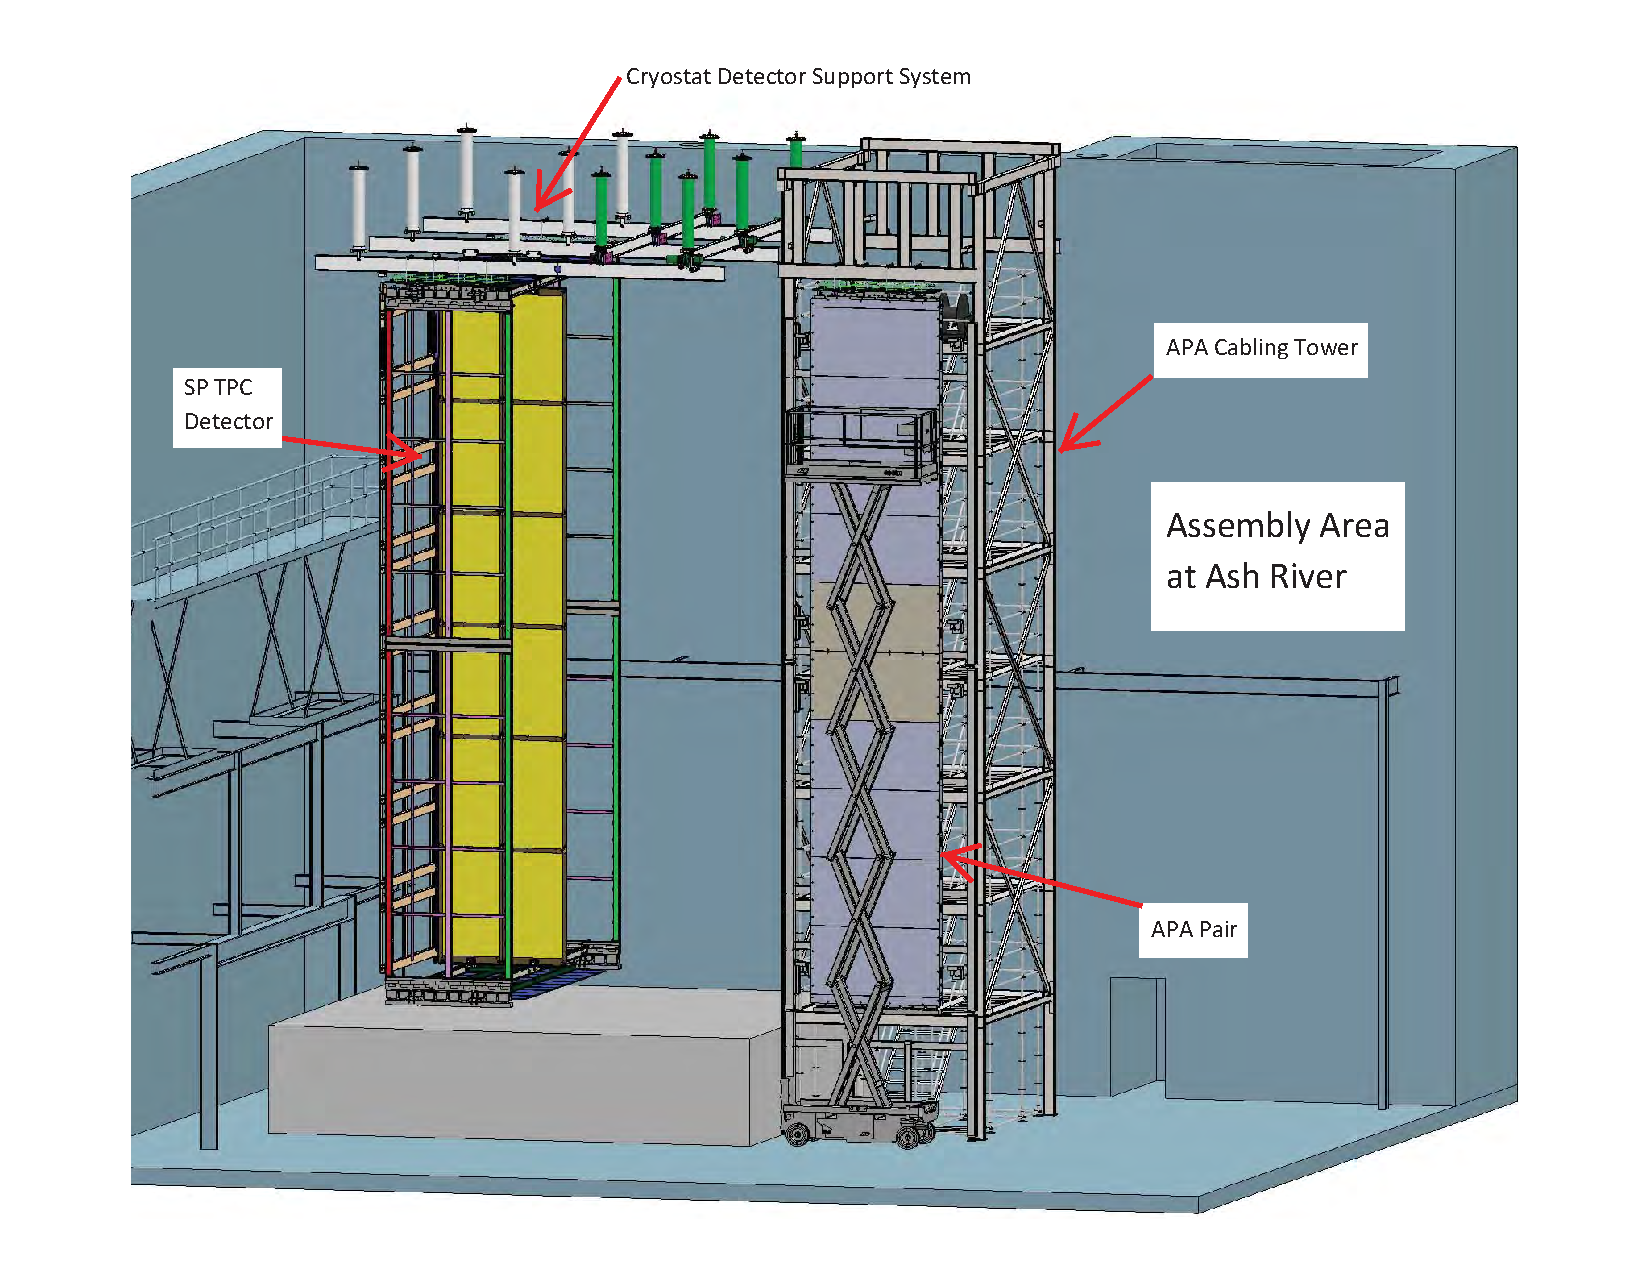
\includegraphics[width=0.8\textwidth,trim=0pt 0pt 0pt 0pt,clip]
{DUNE-Trial-Assembly-Ash-River}
%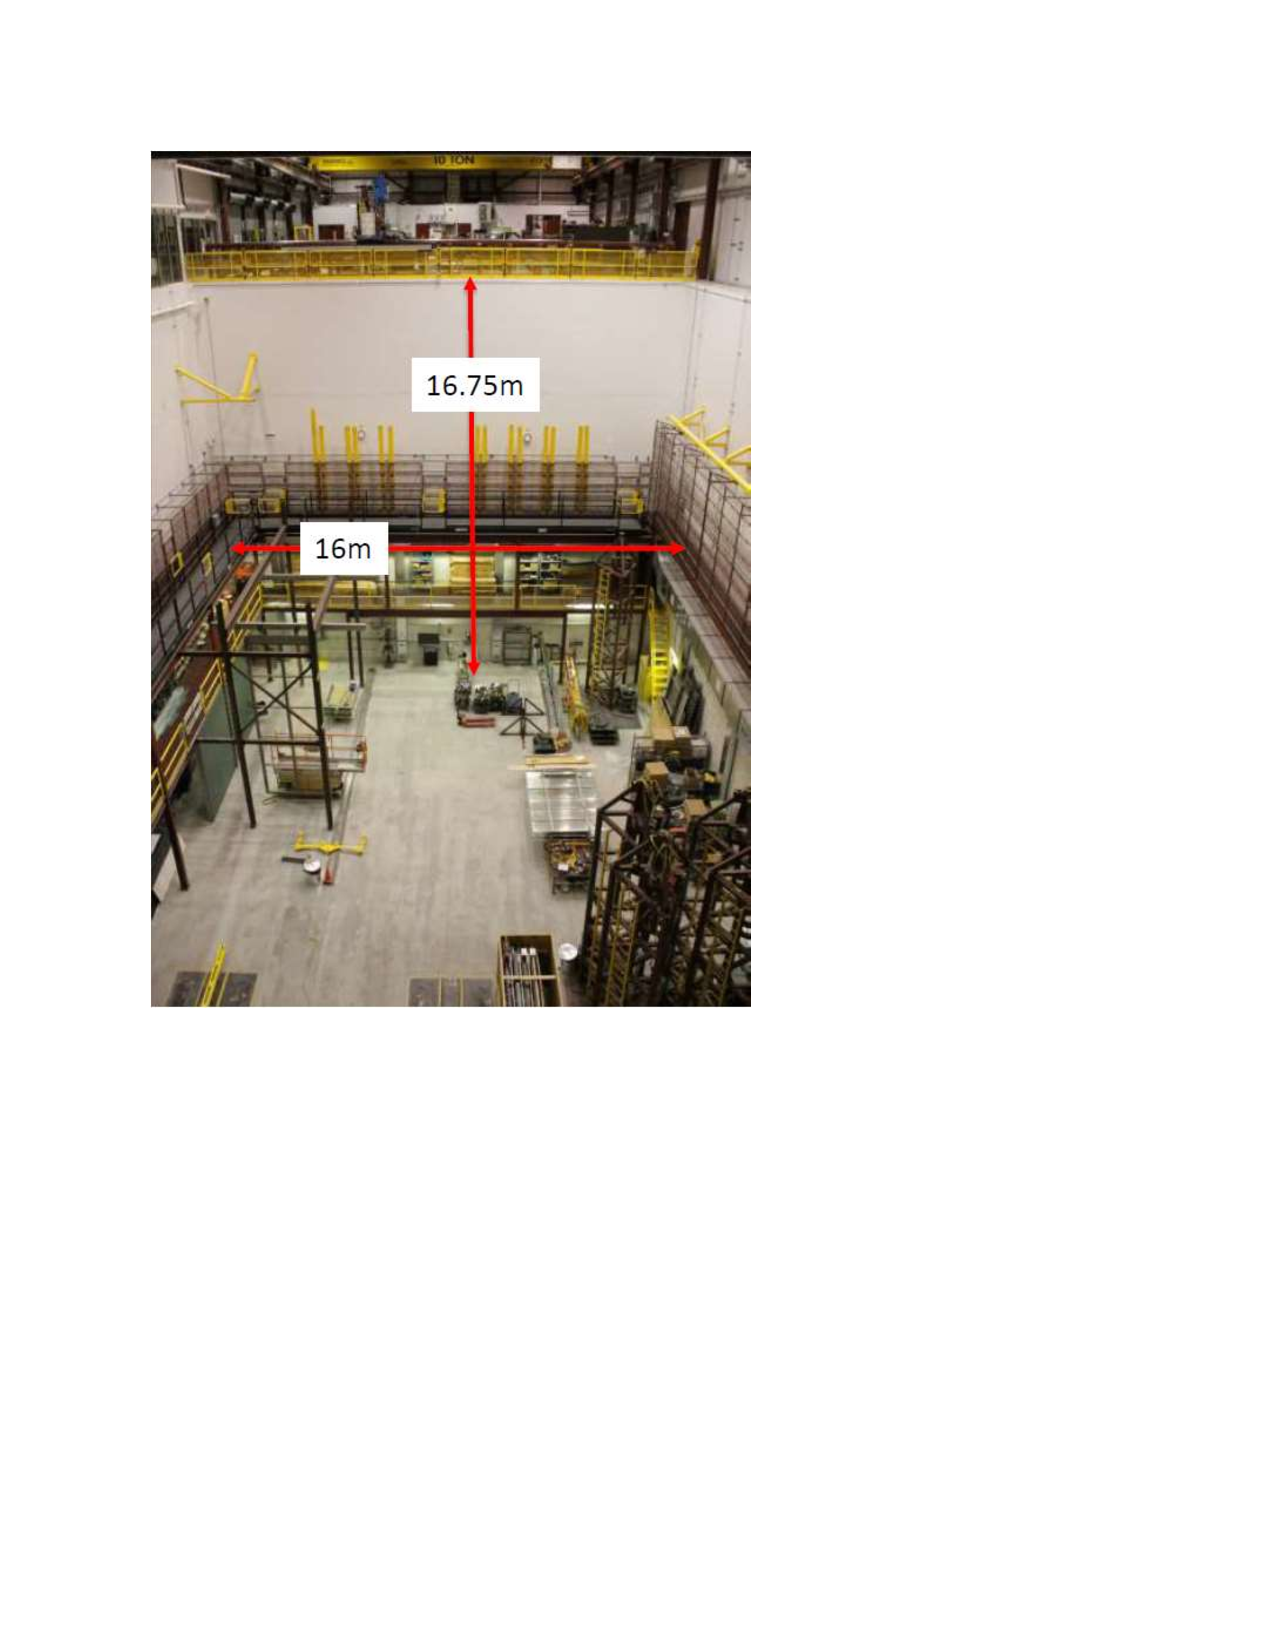
\includegraphics[width=0.49\textwidth,trim=0pt 300pt 180pt]{NOvA-Assembly-Area}
\end{dunefigure}




The \nova Far Detector Laboratory at Ash River is owned and operated by the University of Minnesota using grants from the DOE and Fermilab. The Trial Assembly program for both \dword{protodune} and \dword{dune} are here. During \dword{protodune} detector design, many of the installation and deployment concepts were tested and modified here. Experience showed that one had to attempt different concepts with full-scale mechanical components. Hazard analysis and procedure documents were developed, and hands on working group meetings with the different consortia were held.  The lessons learned and training from the trial assembly helped ensure that the assembly and integration for \dword{protodune} went well at CERN.

While the University of Minnesota has jurisdiction over the safety program at Ash River, we also follow the Fermilab Safety Program and work together to ensure a safe working environment.  
One key attribute of the \dword{protodune} work was compiling sets of documentation from component design to hazard analysis to final assembly procedures for approval by the CERN Health Safety and Environment division. 
For Ash River and \dword{dune}, this is all part of the Operational Readiness Clearance (ORC) review process. 
Documentation for both the trail assembly process at Ash River and for \dword{dune} will be stored on the \dword{edms} at CERN. 
Though many of the \dword{tpc} components are mechanically similar to the \dword{protodune} components, the access equipment will be different and the need to work at \SI{14}{m} will make construction of the \dword{dune} single phase detector much more challenging.  
The \nova Far Detector assembly area (see Figure~\ref{fig:NOvA-Assembly-Area}) has both the elevation and floor space available to do a full-scale test of both the assembly stations and a portion of the inside of the \dword{dune} cryostat. 

%\begin{dunefigure}[DUNE - Trail Assembly at Ash River] %%this gets %sniffed for table of figures
%{fig:DUNE-Trial-Assembly-Ash-River}  %this is figure name %and is %what the above \ref:{fig:...} matches 
%{DUNE trial assembly at Ash River}  %this is caption
%\centering
%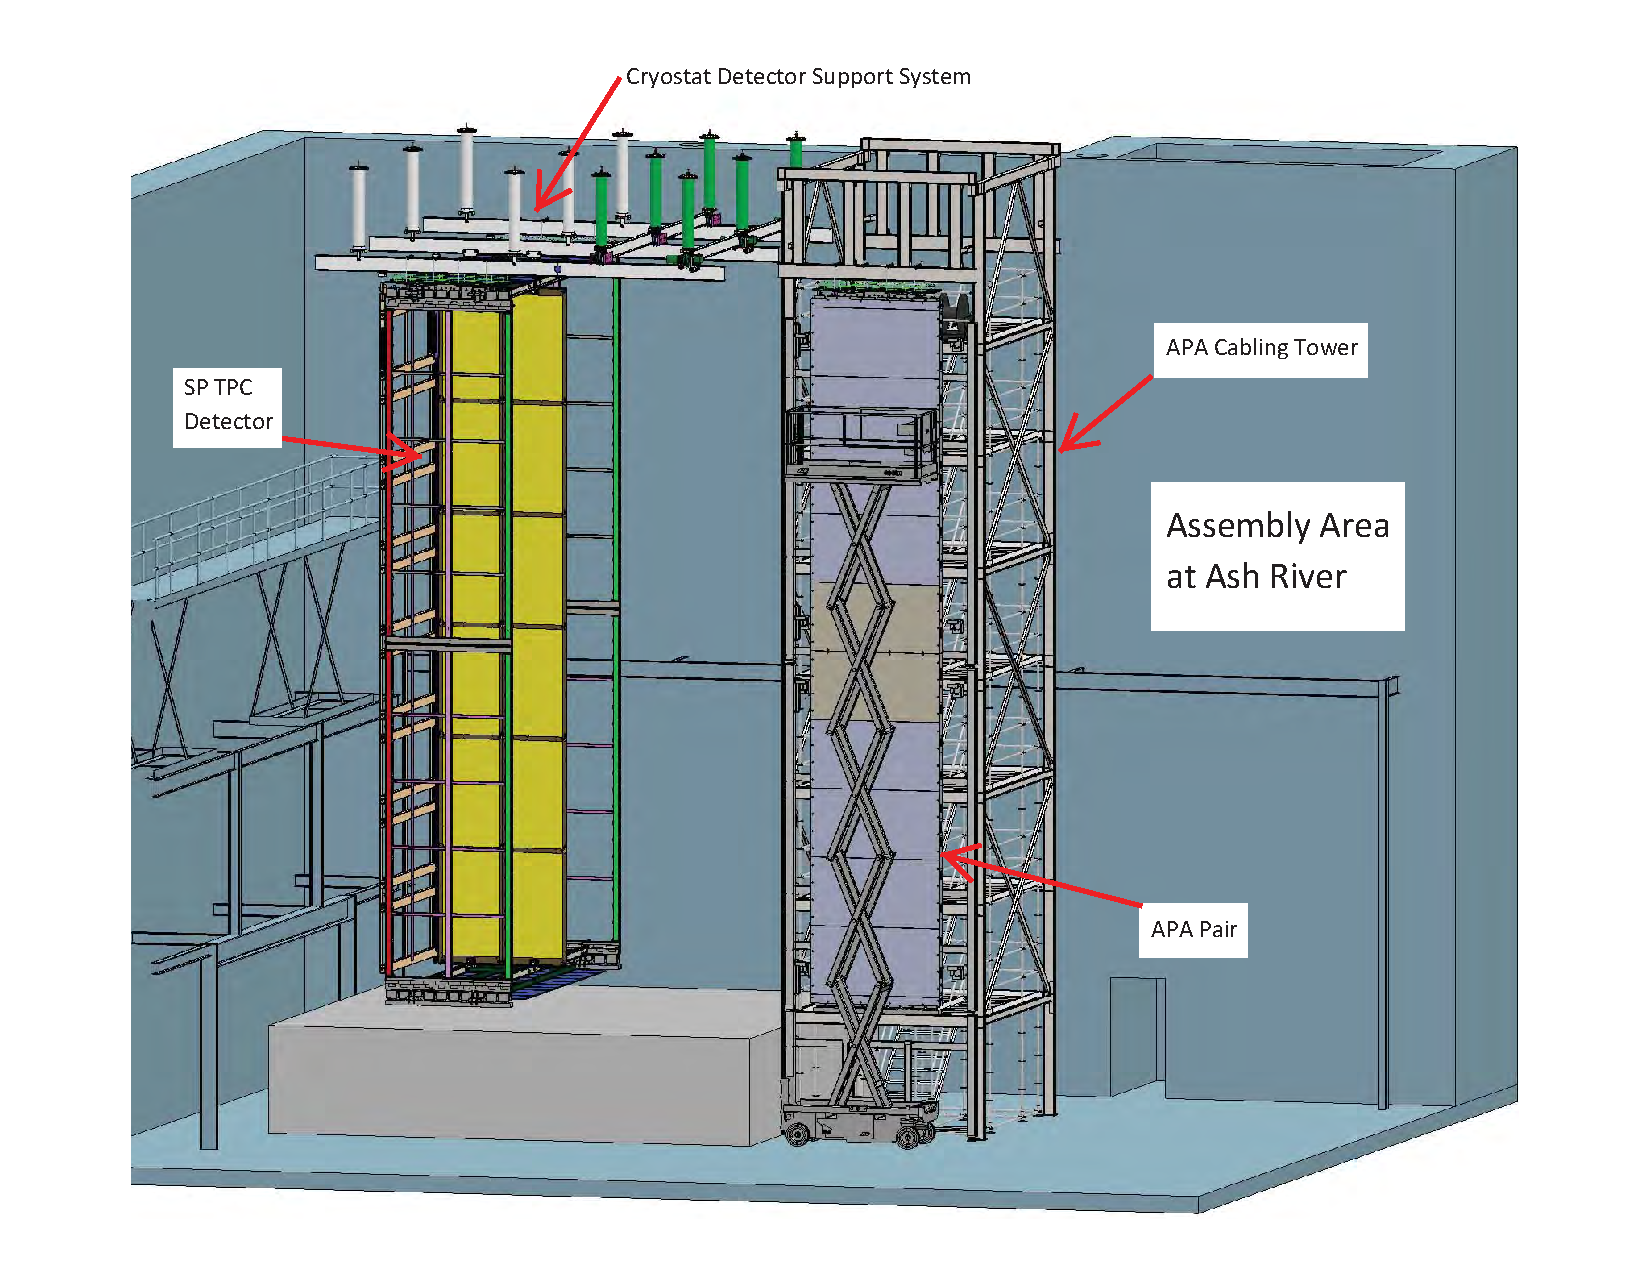
\includegraphics[width=0.7\textwidth,trim=0pt 0pt 0pt %0pt,clip]{DUNE-Trial-Assembly-Ash-River}
%\end{dunefigure}

At Ash River, we also have a 75 \si{ft} $\times$  100 \si{ft} loading dock and ramp access, two 10-ton cranes, a machine shop, and wide assortment of tools.  Add an experienced crew of technicians who all had several months at CERN building \dword{protodune} as well as fabricating experience makes Ash River a good facility for these tasks. 
The \dword{dune} \dword{fd} trial assembly program at Ash River has the following goals:

\begin{enumerate}
\item Test all full scale \dword{tpc} components during assembly stages and inside the cryostat:  
\begin{itemize}
    \item \dword{apa}  assembly: manipulation of \dword{apa} shipping frames, joining an \dword{apa} pair together, \dword{ce} cabling, \dword{apa} protection, movement on shuttle beam, cryostat cabling, and final deployment in cryostat. 
    \item Integration and installation testing of \dword{pd} (Photon Detector) components: cable harness routing and cryogenic cable strain relief, module integration into \dword{apa} frames, and electrical connections between upper and lower \dword{apa}s.  In addition, \dword{pd} monitoring system components mounting and optical fiber routing on the \dword{cpa} will be tested.
    \item \dword{dss} and shuttle beam system, including final detector configuration.
    \item Assembly of \dword{hv} system: construction of an endwall, \dword{cpa} pairs, movement on shuttle beam, and final deployment in cryostat.
    \item Future assembly of dual phase detector components.
\end{itemize}
\item Write full set of hazard analyses and assembly procedure documents, including gathering all component documentation. 
\item Test access equipment (scaffold, scissor lifts, work platforms) and lifting fixtures. 
\item Study assembly time and motion, including labor estimates. This facility can also be used as a training site for lead workers as \dword{dune} begins set up and for testing mechanical modifications.
\end{enumerate}

In order to meet the goals a testing program has been developed to perform sequentially more sophisticated and complete tests over time. 
This program, which is summarized in Table \ref{tab:AR-test-program}, begins with simple tests that can be done with minimal equipment and builds to a fairly complete installation test with realistic prototype components and geometrical layout. 
The 3-D model in Figure \ref{fig:NOvA-Assembly-Area} represents the final stage of the test setup.

\begin{dunetable}
[Summary of the tests at Ash River]
{p{.2\textwidth}p{.7\textwidth}} %{ll}
{tab:AR-test-program}
{Summary of the tests at Ash River} 
Testing phase & Test description\\ \toprowrule
FY-19 Phase 0   &  \\ \colhline
 & Test FC Deployment and Ground Plane installation \\ \colhline
 & Check Vertical cabling with a pair of APA side tubes \\ \colhline
 & Build an APA Cabling tower for full scale APA pair assembly \\ \colhline
 & Build a CPA assembly stand and test assembly process \\ \colhline
  & Test APA Shipping Frame \\ \colhline
  FY-20 21 Phase 1 &  \\ \colhline
  & Build support structure for DSS shuttle, 3 sections of DSS beam \\ \colhline
  &  Test movement of CPA and APA from cleanroom to final destination\\ \colhline
  & Test APA, CPA, Endwall and FC deployment in one drift section \\ \colhline
  & Test assembly sequence of final section of TPC \\ \colhline
  & Removal of DSS shuttle beam runway rails \\ \colhline
  & Final deployment after TCO is closed up \\ \colhline
  FY-22 thru FY23 Phase 2&  \\ \colhline
  &  Include the top of the cryostat ( no warm structure) with \fdth \\
  \colhline
  & Test DSS installation  \\  \colhline
  &  Test CE cable installation using \fdth \\  \colhline
  & Design \fdth to support Dual Phase installation test \\ \colhline
  & Test shipping and construction using first factory TPC components  \\ \colhline
  & Train lead workers for underground at SURF \\ \colhline

\end{dunetable}

\subsubsection{DAQ QC testing}

Testing is required at several stages of \dword{daq} installation.  The first is the installation of the dataroom infrastructure, where cooling water leak checking, rack airflow, and power distribution will be tested upon installation by professional data center building contractors.

The detector-to-dataroom multimode fiber will run close to its optical power budget.  This fiber is routed from the \dwords{wib} on top of the cryostat to the servers in the \dword{cuc}, so it must be installed and tested by fiber professionals early in the process.  Covered cable trays will protect it after installation.  As \dword{apa}s and servers are commissioned, pre-tested fibers will be connected to the newly installed hardware.

The \dword{daq} servers in the \dword{cuc} dataroom will be initially received and integrated off site.  Upon installation in the \dword{cuc}, only a simple functionality test will be needed.  Sufficient spare capacity will be installed, and the main commissioning work will be software related and can be done over the network from the surface or remotely.

\subsubsection{APA QC testing}

Once the \dword{apa}s have been installed, the only relevant test for \dword{apa} quality is the tension measurement of the wires. 
Note that testing the \dword{ce} will directly inform wire continuity and the full function of the channels, so only the tension remains to be tested. 
The current plan is to re-test a sub-fraction of the 350 wires that were measured at the \dword{itf} using the laser method. 
The exact number or wires to test will depend on the final schedule for underground testing. 
Two alternatives for tension measurement are under development. 
One uses an electrical signal that would allow us to measure a much larger fraction of wire tension (and potentially all of them). 
The other uses the \dword{ce} readout to extract the tension from wire movement. 
The second method would allow us to measure all the wires in a short time.

\subsubsection{\dword{hv} QC testing}

The endwalls are assembled in eight panel units, four on each end of the \dword{tpc}.  
As each of the eight panels are removed from the shipping crate and placed on the installation cart, the endwall panel checklist is filled out.\cite{bib:docdb10452}
This checklist includes a visual inspection of the frames, profiles, and connections, as well as continuity and resistance measurements of the divider boards and their connections.  
After completing an eight panel endwall in the cryostat, the complete endwall checklist is filled out.  
This includes hanging position, straightness measurements, and continuity checks between panels.

The \dword{cpa} panels are assembled from three units removed from the shipping crates.  
After each unit is removed from its bag, a visual inspection confirms structural integrity and the connections between \dwords{fss}, \dword{hv} bus pieces, and profiles if present.  
After inspection, the unit is positioned on the \dword{cpa} assembly tower.  
After all three units are connected on the tower, the \dword{cpa} panel checklist is filled out.  
This includes inspecting all mechanical connections, continuity checks of the \dword{fss}, \dword{rp}, profile, and \dword{hv} bus connections, and resistance measurements of the four mini-resistor board connections from the \dword{rp} to the \dword{fss}.  
This is repeated for the second panel in a \dword{cpa} plane.  Then the two panels are paired, each hanging from trolleys on the transport beam.  
Visual inspection of the alignment and hanging straightness are made and \dword{hv} bus connections at the top and bottom are made and checked for continuity (\dword{cpa} plane checklist).

The \dword{fc} top and bottom units are removed from their crates.  The \dword{fc} unit checklist is filled out with a visual inspection of the frames, profiles, and connections, as well as continuity and resistance measurements of the divider boards and their connections.  
After hanging the top \dword{fc} units on the \dword{cpa} plane, the four jumpers from the first \dword{fc} profile on each side of the \dword{cpa} and the \dword{cpa} \dword{fss} is connected, and the resistance is measured, completing the \dword{cpa}/\dword{fc} top assembly checklist. 
The \dword{fc} bottom units are not attached to the \dword{cpa} but are taken into the cryostat independently after filling out the \dword{fc} unit checklist.

The \dword{cpa}/\dword{fc} top assembly is moved into its position in the cryostat.   
After deploying the \dword{fc} top units, the resistor board/jumper between the \dword{fc} and the \dword{cpa} \dword{fss} are visually inspected.  
Also, the latch at the \dword{fc}/\dword{apa} is visually inspected.  After deploying the \dword{fc} bottoms, visual inspection verifies the resistor board/jumper connection from the \dword{fc} to the \dword{cpa}.  
Also, the latch connecting the \dword{fc} bottom to the \dword{apa} is visually inspected.  
These are included in the \dword{cpa}/\dword{fc} cryostat checklist.

\subsubsection{CE QC testing}
Details of the \dword{ce} \dword{qc} testing are  in the \dword{ce} chapter.

\subsubsection{CISC QC testing}

Cryogenics instrumentation systems must undergo a series of tests to guarantee they will perform as expected:  

\begin{itemize}
\item {\bf Purity Monitors}: Each of the fully assembled purity monitor arrays is placed in its shipping tube, which serves as a vacuum chamber to test all electric and optical connections at \surf before the system is inserted into the cryostat. During insertion, electrical connections are tested continuously with multimeters and electrometers.

\item {\bf Static T-gradient Thermometers}: Right after each sensor array is installed, its verticality 
is checked, and the tensions in the stainless steel strings adjusted as necessary. Once cables are routed to the corresponding \dword{dss} ports, the entire readout chain is tested. This allows a test of the sensor, the sensor-connector assembly, the cable-connector assemblies at both ends, and the noise level inside the cryostat.
If any sensor presents a problem, it is replaced. If the problem persists, the cable is checked and replaced as needed.

\item {\bf Dynamic T-gradient Thermometers}: The full system is tested after it is installed in the cryostat. Two aspects are particularly important: the vertical motion of the system using the step motor, which is controlled through the slow controls system, and the full readout chain, which will be tested mainly for failures in sensors, cables, and connectors inside the cryostat. 

\item {\bf Individual Sensors}: To address the quality of individual precision sensors, the same method is used as for
the static T-gradient monitors. For standard \dwords{rtd} to be installed on the cryostat walls, floor, and roof, calibration is not an issue. Any \dword{qc} required for associated cables and connectors is performed following the same procedure as for precision sensors.

\item {\bf Gas Analyzers}: Once the gas analyzer modules are installed at \surf and before the cryostat is commissioned, the analyzers 
are checked for both \textit{zero} and the \textit{span} values using a gas-mixing instrument and two gas cylinders, one with a
zero level of the gas analyzer contaminant species and the other with a known percentage of the contaminant gas. This verifies that the gas analyzers are operating properly. 

\item {\bf Liquid Level Monitoring}: Once installed in the four cryostat corners, the capacitive level meters are tested in situ 
using a suitable dielectric in contact with the sensors.

\item {\bf Cameras}: After installing and connecting the wiring, fixed cameras, movable inspection cameras, and the light-emitting system are checked for operation at room temperature. Good quality images should be obtained of all cryostat and detector areas chosen from the system's design. The system for moving inspection cameras should behave as expected.  
\end{itemize}

\subsubsection{Photon QC testing}

Access to the \dwords{pd} inside the \dword{apa}s is severely limited once the \dword{ce} cable conduit is in place, so identifying problems early in the process is necessary to minimize schedule issues caused by required \dword{pd} maintenance or repair due to problems detected during installation.

Once integrated \dword{apa}s are received in the \dword{sas} for the cleanroom in front of the cryostat, an electrical connectivity test between the cable end exiting the \dword{apa} to be installed and each of the \dword{pd} modules in that \dword{apa} will be performed.  Discussions are underway with the \dword{apa} consortium to determine if the transport frames for shipping the integrated \dword{apa} pairs can be made sufficiently light-tight to allow biasing the photosensors and checking that they are operating properly.  Accessing the \dword{pd} modules involves removing the \dword{ce} cable conduits from the \dword{apa} side tubes, so this is the last time in the installation process that \dwords{pd} can be reached for repair or replacement.  Any repairs to the \dword{pd} system discovered later in the installation process would require returning the \dword{apa} module to this point in the installation sequence.

As the upper and lower \dword{apa}s are joined on the assembly tower, photon detector cables from the upper to the lower \dword{apa} will be connected, and at that time, continuity checks will be made.

Once the upper and lower \dword{apa}s are joined, the assembled unit will be moved into a coldbox in front of the cryostat for final testing.  This is an opportunity to make a final low-temperature check of the complete \dword{pd} \dword{ce} and cabling chain before installation into the cryostat.  \dword{pd} \dword{fe} electronics boards will be used to read out the photon system during the cold test, and results willl be compared to previous \dword{qa} test results.

The \dword{apa} stack is rolled into position in the cryostat following the coldbox test, and the \dword{pd} and \dword{ce} cables connected to the cryostat flange.  At this point, a final continuity check is made from the flange bulkhead to the \dword{pd} module.

Discussions are underway with the installation team to arrange for a one-shift dark test of the installed photon detectors in the cryostat following final installation, verifying end-to-end system operation.

\subsubsection{Calibration system testing}
The laser system is aligned and tested as the lasers are installed. This requires and initial alignment with the alignment laser then testing with the UV laser under controlled conditions. Details of the testing procedures have not yet been developed. The pulsed neutron source will be calibrated offline to verify the shielding design and neutron flux. {\it In situ} the source will be operated in test mode to verify the functionality. 

%%%%%%%%%%%%%%%%%%%%%%%%%%%%
\subsection{Environmental, Safety, and Health (ES\&H)}
\label{sec:fdsp-tc-inst-safety}

Fermilab, \fixme{SURF and?}  and \dword{dune} are committed to supporting the health and safety of staff, the community, and the environment in research and operations, as stated in the \dword{lbnf}/\dword{dune} Integrated Safety Management Plan\cite{bib:docdb291}. The safety and health program complies with applicable standards and local, state, and federal legal requirements through Fermilab's Work Smart Set of Standards \fixme{ref -ask Mike A} and the contract between \dword{fra} and the \dword{doe}. \dword{fnal} and the \dword{sdsd} have the host laboratory responsibilities for \dword{lbnf} and \dword{dune} operations at \dword{surf} in Lead, South Dakota.
The Fermilab facilities are further subject to the requirements of the \dword{doe} Workers Safety and Health Program 10 CFR 851\cite{doe-10cfr851}. These requirements are promulgated through the Fermilab Directors Policy Manual, and the \dword{feshm}, which align with the \dword{surf} \dword{esh} manual.

%While \dword{esh} will be  a host laboratory (Fermilab/SDSD) responsibility, a  Global Safety Coordination group will evaluate applicable codes and standards including international code equivalency for the design, assembly, and installation of the \dword{dune} detectors. The Global Safety Coordination group is  a team of engineering and \dword{esh} experts from within \dword{lbnf} and \dword{dune} organizations.  These requirements will be adopted by \dword{dune}, JPO (Joint Project Office), and \dword{lbnf} organizations and used to develop manufacturing, assembly, and installation processes and procedures. 
While \dword{esh} is  a host laboratory (\dword{fnal}'s \dword{sdsd}) responsibility, a  \dword{gsc} will evaluate applicable codes and standards including international code equivalency for the design, assembly, and installation of the \dword{dune} \dwords{detmodule}. The \dword{gsc} is  a team of engineering and \dword{esh} experts from within \dword{lbnf} and \dword{dune} organizations.  These requirements will be adopted by \dword{dune}, \dword{jpo}, and \dword{lbnf} organizations and used to develop manufacturing, assembly, and installation processes and procedures. 
\dword{dune} will develop an %Installation 
\dword{esh} plan for installation that will define %a specific set of 
the \dword{esh} requirements and responsibilities that personnel will be required to follow while  assembling, installing, and constructing equipment at \dword{surf}. % and \dword{itf}. 

{\bf Work Planning and Controls:} The goal of the work planning and \dword{ha} process is to initiate thought about the hazards associated with work activities and how the work can be performed safely. Careful planning of a job assures that it is performed efficiently and safely. Work planning ensures the scope of the job is understood, appropriate materials and tools are available, all hazards have been identified, mitigation efforts established, and all affected employees understand what is expected of them. %\dword{ha} is a critical part of work planning.  
The Work Planning and Hazard Analysis program is documented in Chapters 2060 in the \dword{feshm}.

The shift supervisor will lead %daily 
work planning meetings at the start of each shift to coordinate work activities, review hazards and mitigations, and answer any questions.

{\bf Documentation Approval Process:} The engineering review and approval process of all required documentation includes structural calculations, assembly drawings, load tests, \dwords{ha}, and procedural documents for \fixme{a set of identified?} typical individual tasks.  For the larger operations and systems like \dword{tpc} component factories, the \dword{dss}, cleanroom, and assembly infrastructure, this will be followed by an \dword{orr} by a joint safety committee that visits the site  after reviewing the documentation, and watches the full operation before signing off on the documentation.

{\bf \dword{esh} Support:} Safety starts from the ground up, both on the surface and in the underground facilities. All employees have work stop authority in support of  a safe working environment. Personnel will need to use the necessary \dword{ppe} identified through the \dword{ha} process for the task. A local \dword{esh} coordinator under the direction of the \dword{dune} \dword{esh} Manager will provide daily support for the facilities and attend the %daily 
\fixme{they are either daily or per shift - sounds like `per shift' is correct}
work planning meetings to notify each shift of potential safety issues and constraints, to ensure that  employees have the necessary \dword{esh} training, and to be responsible \fixme{to make sure the workers are responsible? or so that  the coordinator has what they need so that they can be responsible?} for managing \dword{esh} related  documentation including training records, weekly safety reports, near miss and accident reports, and equipment inspection.

{\bf Work Underground} \dword{sdsta} will maintain:
\begin{itemize}
    \item Site Access Control Program through \dwords{tap};
    \item \dword{em} program, which includes an Emergency Response incident command system and an \dword{ert}.  Typically, a small number of employees underground (guides) are also training as first responders to help in a medical emergency.
    
\end{itemize}

{\bf Equipment operation:} All overhead cranes, gantry cranes, fork lifts, motorized equipment trains/carts will be operated only by trained licensed operators. 
Other equipment, e.g., scissor lifts, pallet jacks, hand tools, and shop equipment, may only be operated by people trained
and certified for the particular piece of equipment.

{\bf House cleaning:} All workers underground are responsible for keeping a clean organized work area. Flammable items must be in proper storage cabinets, and items like empty shipping crates and boxes must be removed and %shipped 
transported back to the surface to make space.

{\bf \dword{ppe}:} 
\dword{ppe} is the responsibility of the host laboratory,  %(Fermilab/SDSD) and will be supplied 
which will supply it to all workers. 

{\bf Access and training:}  All \dword{dune} workers requiring access to the \dword{surf} site must (1) register through the \dword{fnal} Users Office to receive the necessary user training and a \dword{fnal} ID number, and they must apply for a \dword{surf} identification badge. % for \dword{dune} activities. 
All \dword{dune} workers will be required to complete \dword{surf} Surface and Underground Orientation classes. Workers accessing the underground must also complete 4850 and 4910 level specific unescorted access training. %A guide must be stationed on all working levels and have received the necessary guide training. 
A properly trained guide will be stationed on all working levels. 

{\bf Requirements at collaborating %laboratories and 
institutions:} All work performed at collaborating institutions will be completed in accordance with the %collaborating 
institution's \dword{esh} policies and programs. 
Equipment and operating procedures provided by the %collaborating 
institution must conform to the \dword{dune} Project \dword{ieshp}. %\dword{esh} and Integrated Safety Management policies and procedures. 
The %collaborating 
institution's \dword{esh} department is responsible for providing \dword{esh}  oversight for all work activities carried out in their facilities. % in collaborating institution facilities. 
\dword{lbnf} and \dword{dune} personnel will also follow the \dword{esh} manual and procedures of the collaborating institutions.


%%%%%%%%%%%%%%%%%%%%%%%%%%%%
%\subsection{Costs, Schedule and Risk Analysis} MOVED TO NEW CHAPTER



%\subsection{Conclusions}
%\label{sec:fdsp-tc-inst-concl}

%That's all folks
%The End
%\fixme{contribution from editors}